%%%%%%%%%%%%%%%%%%%%%%%%%%%%%%%%%%%%%%%%%
%  My documentation report
%  Objetive: Explain what I did and how, so someone can continue with the investigation
%
% Important note:
% Chapter heading images should have a 2:1 width:height ratio,
% e.g. 920px width and 460px height.
%
%%%%%%%%%%%%%%%%%%%%%%%%%%%%%%%%%%%%%%%%%

%----------------------------------------------------------------------------------------
%	PACKAGES AND OTHER DOCUMENT CONFIGURATIONS
%----------------------------------------------------------------------------------------

\documentclass[11pt,fleqn]{book} % Default font size and left-justified equations

% \setlength{\parskip}{\baselineskip}%
% \setlength{\parindent}{0pt}%

\usepackage[top=3cm,bottom=3cm,left=3.2cm,right=3.2cm,headsep=11pt,letterpaper]{geometry} % Page margins

\usepackage{xcolor} % Required for specifying colors by name
\definecolor{ocre}{RGB}{52,177,201} % Define the orange color used for highlighting throughout the book

% Font Settings
\usepackage{avant} % Use the Avantgarde font for headings
%\usepackage{times} % Use the Times font for headings
\usepackage{mathptmx} % Use the Adobe Times Roman as the default text font together with math symbols from the Sym­bol, Chancery and Com­puter Modern fonts

\usepackage{microtype} % Slightly tweak font spacing for aesthetics
\usepackage[utf8]{inputenc} % Required for including letters with accents
\usepackage[T1]{fontenc} % Use 8-bit encoding that has 256 glyphs

\usepackage{graphicx}
\usepackage{epstopdf}
% Bibliography
\usepackage[style=alphabetic,sorting=nyt,sortcites=true,autopunct=true,autolang=hyphen,hyperref=true,abbreviate=false,backref=true,backend=biber]{biblatex}
\addbibresource{bibliography.bib} % BibTeX bibliography file
\defbibheading{bibempty}{}


% marcas de modificaciones
\newcommand{\trg}[1]{\textcolor{red}{#1}}


%----------------------------------------------------------------------------------------
%	VARIOUS REQUIRED PACKAGES
%----------------------------------------------------------------------------------------

\usepackage{titlesec} % Allows customization of titles

\usepackage{graphicx} % Required for including pictures
\graphicspath{{Pictures/}} % Specifies the directory where pictures are stored

\usepackage{lipsum} % Inserts dummy text

\usepackage{tikz} % Required for drawing custom shapes

\usepackage[spanish]{babel} % English language/hyphenation

\usepackage{enumitem} % Customize lists
\setlist{nolistsep} % Reduce spacing between bullet points and numbered lists

\usepackage{booktabs} % Required for nicer horizontal rules in tables

\usepackage{eso-pic} % Required for specifying an image background in the title page

%----------------------------------------------------------------------------------------
%	MAIN TABLE OF CONTENTS
%----------------------------------------------------------------------------------------

\usepackage{titletoc} % Required for manipulating the table of contents
\addto\captionsenglish{%
  \renewcommand{\contentsname}{Contenido}%
}

\contentsmargin{0cm} % Removes the default margin
% Chapter text styling
\titlecontents{chapter}[1.25cm] % Indentation
{\addvspace{15pt}\large\sffamily\bfseries} % Spacing and font options for chapters
{\color{ocre!60}\contentslabel[\Large\thecontentslabel]{1.25cm}\color{ocre}} % Chapter number
{}  
{\color{ocre!60}\normalsize\sffamily\bfseries\;\titlerule*[.5pc]{.}\;\thecontentspage} % Page number
% Section text styling
\titlecontents{section}[1.25cm] % Indentation
{\addvspace{5pt}\sffamily\bfseries} % Spacing and font options for sections
{\contentslabel[\thecontentslabel]{1.25cm}} % Section number
{}
{\sffamily\hfill\color{black}\thecontentspage} % Page number
[]
% Subsection text styling
\titlecontents{subsection}[1.25cm] % Indentation
{\addvspace{1pt}\sffamily\small} % Spacing and font options for subsections
{\contentslabel[\thecontentslabel]{1.25cm}} % Subsection number
{}
{\sffamily\;\titlerule*[.5pc]{.}\;\thecontentspage} % Page number
[] 

%----------------------------------------------------------------------------------------
%	MINI TABLE OF CONTENTS IN CHAPTER HEADS
%----------------------------------------------------------------------------------------

% Section text styling
\titlecontents{lsection}[0em] % Indendating
{\footnotesize\sffamily} % Font settings
{}
{}
{}

% Subsection text styling
\titlecontents{lsubsection}[.5em] % Indentation
{\normalfont\footnotesize\sffamily} % Font settings
{}
{}
{}
 
%----------------------------------------------------------------------------------------
%	PAGE HEADERS
%----------------------------------------------------------------------------------------

\usepackage{fancyhdr} % Required for header and footer configuration

\pagestyle{fancy}
\renewcommand{\chaptermark}[1]{\markboth{\sffamily\normalsize\bfseries\thechapter.\ #1}{}} % Chapter text font settings
% \renewcommand{\chaptermark}[1]{\markboth{\sffamily\normalsize\bfseries\chaptername\ \thechapter.\ #1}{}} % Chapter text font settings
\renewcommand{\sectionmark}[1]{\markright{\sffamily\normalsize\thesection\hspace{5pt}#1}{}} % Section text font settings
\fancyhf{} \fancyhead[LE,RO]{\sffamily\normalsize\thepage} % Font setting for the page number in the header
\fancyhead[LO]{\rightmark} % Print the nearest section name on the left side of odd pages
\fancyhead[RE]{\leftmark} % Print the current chapter name on the right side of even pages
\renewcommand{\headrulewidth}{0.5pt} % Width of the rule under the header
\addtolength{\headheight}{2.5pt} % Increase the spacing around the header slightly
\renewcommand{\footrulewidth}{0pt} % Removes the rule in the footer
\fancypagestyle{plain}{\fancyhead{}\renewcommand{\headrulewidth}{0pt}} % Style for when a plain pagestyle is specified

% Removes the header from odd empty pages at the end of chapters
\makeatletter
\renewcommand{\cleardoublepage}{
\clearpage\ifodd\c@page\else
\hbox{}
\vspace*{\fill}
\thispagestyle{empty}
\newpage
\fi}

%----------------------------------------------------------------------------------------
%	THEOREM STYLES
%----------------------------------------------------------------------------------------

\usepackage{amsmath,amsfonts,amssymb,amsthm} % For math equations, theorems, symbols, etc

\newcommand{\intoo}[2]{\mathopen{]}#1\,;#2\mathclose{[}}
\newcommand{\ud}{\mathop{\mathrm{{}d}}\mathopen{}}
\newcommand{\intff}[2]{\mathopen{[}#1\,;#2\mathclose{]}}
\newtheorem{notation}{Notation}[chapter]

%%%%%%%%%%%%%%%%%%%%%%%%%%%%%%%%%%%%%%%%%%%%%%%%%%%%%%%%%%%%%%%%%%%%%%%%%%%
%%%%%%%%%%%%%%%%%%%% dedicated to boxed/framed environements %%%%%%%%%%%%%%
%%%%%%%%%%%%%%%%%%%%%%%%%%%%%%%%%%%%%%%%%%%%%%%%%%%%%%%%%%%%%%%%%%%%%%%%%%%
\newtheoremstyle{ocrenumbox}% % Theorem style name
{0pt}% Space above
{0pt}% Space below
{\normalfont}% % Body font
{}% Indent amount
{\small\bf\sffamily\color{ocre}}% % Theorem head font
{\;}% Punctuation after theorem head
{0.25em}% Space after theorem head
{\small\sffamily\color{ocre}\thmname{#1}\nobreakspace\thmnumber{\@ifnotempty{#1}{}\@upn{#2}}% Theorem text (e.g. Theorem 2.1)
\thmnote{\nobreakspace\the\thm@notefont\sffamily\bfseries\color{black}---\nobreakspace#3.}} % Optional theorem note
\renewcommand{\qedsymbol}{$\blacksquare$}% Optional qed square

\newtheoremstyle{blacknumex}% Theorem style name
{5pt}% Space above
{5pt}% Space below
{\normalfont}% Body font
{} % Indent amount
{\small\bf\sffamily}% Theorem head font
{\;}% Punctuation after theorem head
{0.25em}% Space after theorem head
{\small\sffamily{\tiny\ensuremath{\blacksquare}}\nobreakspace\thmname{#1}\nobreakspace\thmnumber{\@ifnotempty{#1}{}\@upn{#2}}% Theorem text (e.g. Theorem 2.1)
\thmnote{\nobreakspace\the\thm@notefont\sffamily\bfseries---\nobreakspace#3.}}% Optional theorem note

\newtheoremstyle{blacknumbox} % Theorem style name
{0pt}% Space above
{0pt}% Space below
{\normalfont}% Body font
{}% Indent amount
{\small\bf\sffamily}% Theorem head font
{\;}% Punctuation after theorem head
{0.25em}% Space after theorem head
{\small\sffamily\thmname{#1}\nobreakspace\thmnumber{\@ifnotempty{#1}{}\@upn{#2}}% Theorem text (e.g. Theorem 2.1)
\thmnote{\nobreakspace\the\thm@notefont\sffamily\bfseries---\nobreakspace#3.}}% Optional theorem note

%%%%%%%%%%%%%%%%%%%%%%%%%%%%%%%%%%%%%%%%%%%%%%%%%%%%%%%%%%%%%%%%%%%%%%%%%%%
%%%%%%%%%%%%% dedicated to non-boxed/non-framed environements %%%%%%%%%%%%%
%%%%%%%%%%%%%%%%%%%%%%%%%%%%%%%%%%%%%%%%%%%%%%%%%%%%%%%%%%%%%%%%%%%%%%%%%%%
\newtheoremstyle{ocrenum}% % Theorem style name
{5pt}% Space above
{5pt}% Space below
{\normalfont}% % Body font
{}% Indent amount
{\small\bf\sffamily\color{ocre}}% % Theorem head font
{\;}% Punctuation after theorem head
{0.25em}% Space after theorem head
{\small\sffamily\color{ocre}\thmname{#1}\nobreakspace\thmnumber{\@ifnotempty{#1}{}\@upn{#2}}% Theorem text (e.g. Theorem 2.1)
\thmnote{\nobreakspace\the\thm@notefont\sffamily\bfseries\color{black}---\nobreakspace#3.}} % Optional theorem note
\renewcommand{\qedsymbol}{$\blacksquare$}% Optional qed square
\makeatother

% Defines the theorem text style for each type of theorem to one of the three styles above
\newcounter{dummy} 
\numberwithin{dummy}{section}
\theoremstyle{ocrenumbox}
\newtheorem{theoremeT}[dummy]{Theorem}
\newtheorem{problem}{Problem}[chapter]
\newtheorem{exerciseT}{Exercise}[chapter]
\theoremstyle{blacknumex}
\newtheorem{exampleT}{Example}[chapter]
\theoremstyle{blacknumbox}
\newtheorem{vocabulary}{Vocabulary}[chapter]
\newtheorem{definitionT}{Definition}[section]
\newtheorem{corollaryT}[dummy]{Corollary}
\theoremstyle{ocrenum}
\newtheorem{proposition}[dummy]{Proposition}

%----------------------------------------------------------------------------------------
%	DEFINITION OF COLORED BOXES
%----------------------------------------------------------------------------------------

\RequirePackage[framemethod=default]{mdframed} % Required for creating the theorem, definition, exercise and corollary boxes

% Theorem box
\newmdenv[skipabove=7pt,
skipbelow=7pt,
backgroundcolor=black!5,
linecolor=ocre,
innerleftmargin=5pt,
innerrightmargin=5pt,
innertopmargin=5pt,
leftmargin=0cm,
rightmargin=0cm,
innerbottommargin=5pt]{tBox}

% Exercise box	  
\newmdenv[skipabove=7pt,
skipbelow=7pt,
rightline=false,
leftline=true,
topline=false,
bottomline=false,
backgroundcolor=ocre!10,
linecolor=ocre,
innerleftmargin=5pt,
innerrightmargin=5pt,
innertopmargin=5pt,
innerbottommargin=5pt,
leftmargin=0cm,
rightmargin=0cm,
linewidth=4pt]{eBox}	

% Definition box
\newmdenv[skipabove=7pt,
skipbelow=7pt,
rightline=false,
leftline=true,
topline=false,
bottomline=false,
linecolor=ocre,
innerleftmargin=5pt,
innerrightmargin=5pt,
innertopmargin=0pt,
leftmargin=0cm,
rightmargin=0cm,
linewidth=4pt,
innerbottommargin=0pt]{dBox}	

% Corollary box
\newmdenv[skipabove=7pt,
skipbelow=7pt,
rightline=false,
leftline=true,
topline=false,
bottomline=false,
linecolor=gray,
backgroundcolor=black!5,
innerleftmargin=5pt,
innerrightmargin=5pt,
innertopmargin=5pt,
leftmargin=0cm,
rightmargin=0cm,
linewidth=4pt,
innerbottommargin=5pt]{cBox}

% Creates an environment for each type of theorem and assigns it a theorem text style from the "Theorem Styles" section above and a colored box from above
\newenvironment{theorem}{\begin{tBox}\begin{theoremeT}}{\end{theoremeT}\end{tBox}}
\newenvironment{exercise}{\begin{eBox}\begin{exerciseT}}{\hfill{\color{ocre}\tiny\ensuremath{\blacksquare}}\end{exerciseT}\end{eBox}}				  
\newenvironment{definition}{\begin{dBox}\begin{definitionT}}{\end{definitionT}\end{dBox}}	
\newenvironment{example}{\begin{exampleT}}{\hfill{\tiny\ensuremath{\blacksquare}}\end{exampleT}}		
\newenvironment{corollary}{\begin{cBox}\begin{corollaryT}}{\end{corollaryT}\end{cBox}}	

%----------------------------------------------------------------------------------------
%	REMARK ENVIRONMENT
%----------------------------------------------------------------------------------------

\newenvironment{remark}{\par\vspace{10pt}\small % Vertical white space above the remark and smaller font size
\begin{list}{}{
\leftmargin=35pt % Indentation on the left
\rightmargin=25pt}\item\ignorespaces % Indentation on the right
\makebox[-2.5pt]{\begin{tikzpicture}[overlay]
\node[draw=ocre!60,line width=1pt,circle,fill=ocre!25,font=\sffamily\bfseries,inner sep=2pt,outer sep=0pt] at (-15pt,0pt){\textcolor{ocre}{R}};\end{tikzpicture}} % Orange R in a circle
\advance\baselineskip -1pt}{\end{list}\vskip5pt} % Tighter line spacing and white space after remark

%----------------------------------------------------------------------------------------
%	SECTION NUMBERING IN THE MARGIN
%----------------------------------------------------------------------------------------

\makeatletter
\renewcommand{\@seccntformat}[1]{\llap{\textcolor{ocre}{\csname the#1\endcsname}\hspace{1em}}}                    
\renewcommand{\section}{\@startsection{section}{1}{\z@}
{-4ex \@plus -1ex \@minus -.4ex}
{1ex \@plus.2ex }
{\normalfont\large\sffamily\bfseries}}
\renewcommand{\subsection}{\@startsection {subsection}{2}{\z@}
{-3ex \@plus -0.1ex \@minus -.4ex}
{0.5ex \@plus.2ex }
{\normalfont\sffamily\bfseries}}
\renewcommand{\subsubsection}{\@startsection {subsubsection}{3}{\z@}
{-2ex \@plus -0.1ex \@minus -.2ex}
{.2ex \@plus.2ex }
{\normalfont\small\sffamily\bfseries}}                        
\renewcommand\paragraph{\@startsection{paragraph}{4}{\z@}
{-2ex \@plus-.2ex \@minus .2ex}
{.1ex}
{\normalfont\small\sffamily\bfseries}}

%----------------------------------------------------------------------------------------
%	HYPERLINKS IN THE DOCUMENTS
%----------------------------------------------------------------------------------------

% For an unclear reason, the package should be loaded now and not later
\usepackage{hyperref}
%\hypersetup{hidelinks,backref=true,pagebackref=true,hyperindex=true,colorlinks=false,breaklinks=true,urlcolor= ocre,bookmarks=true,bookmarksopen=false,pdftitle={Title},pdfauthor={Author}}
\hypersetup{hidelinks,colorlinks=false,breaklinks=true,urlcolor=ocre,bookmarksopen=false,pdftitle={Title},pdfauthor={Author}}

%----------------------------------------------------------------------------------------
%	CHAPTER HEADINGS
%----------------------------------------------------------------------------------------

% The set-up below should be (sadly) manually adapted to the overall margin page septup controlled by the geometry package loaded in the main.tex document. It is possible to implement below the dimensions used in the goemetry package (top,bottom,left,right)... TO BE DONE

\newcommand{\thechapterimage}{}
\newcommand{\chapterimage}[1]{\renewcommand{\thechapterimage}{#1}}

% Numbered chapters with mini tableofcontents
\def\thechapter{\arabic{chapter}}
\def\@makechapterhead#1{
\thispagestyle{empty}
{\centering \normalfont\sffamily
\ifnum \c@secnumdepth >\m@ne
\if@mainmatter
\startcontents
\begin{tikzpicture}[remember picture,overlay]
\node at (current page.north west)
{\begin{tikzpicture}[remember picture,overlay]
\node[anchor=north west,inner sep=0pt] at (0,0) {\includegraphics[width=\paperwidth]{\thechapterimage}};
%%%%%%%%%%%%%%%%%%%%%%%%%%%%%%%%%%%%%%%%%%%%%%%%%%%%%%%%%%%%%%%%%%%%%%%%%%%%%%%%%%%%%
% Commenting the 3 lines below removes the small contents box in the chapter heading
%\fill[color=ocre!10!white,opacity=.6] (1cm,0) rectangle (8cm,-7cm);
%\node[anchor=north west] at (1.1cm,.35cm) {\parbox[t][8cm][t]{6.5cm}{\huge\bfseries\flushleft \printcontents{l}{1}{\setcounter{tocdepth}{2}}}};
\draw[anchor=west] (5cm,-9cm) node [rounded corners=20pt,fill=ocre!10!white,text opacity=1,draw=ocre,draw opacity=1,line width=1.5pt,fill opacity=.6,inner sep=12pt]{\huge\sffamily\bfseries\textcolor{black}{\thechapter. #1\strut\makebox[22cm]{}}};
%%%%%%%%%%%%%%%%%%%%%%%%%%%%%%%%%%%%%%%%%%%%%%%%%%%%%%%%%%%%%%%%%%%%%%%%%%%%%%%%%%%%%
\end{tikzpicture}};
\end{tikzpicture}}
\par\vspace*{230\p@}
\fi
\fi}

% Unnumbered chapters without mini tableofcontents (could be added though) 
\def\@makeschapterhead#1{
\thispagestyle{empty}
{\centering \normalfont\sffamily
\ifnum \c@secnumdepth >\m@ne
\if@mainmatter
\begin{tikzpicture}[remember picture,overlay]
\node at (current page.north west)
{\begin{tikzpicture}[remember picture,overlay]
\node[anchor=north west,inner sep=0pt] at (0,0) {\includegraphics[width=\paperwidth]{\thechapterimage}};
\draw[anchor=west] (5cm,-9cm) node [rounded corners=20pt,fill=ocre!10!white,fill opacity=.6,inner sep=12pt,text opacity=1,draw=ocre,draw opacity=1,line width=1.5pt]{\huge\sffamily\bfseries\textcolor{black}{#1\strut\makebox[22cm]{}}};
\end{tikzpicture}};
\end{tikzpicture}}
\par\vspace*{230\p@}
\fi
\fi
}
\makeatother % Insert the commands.tex file which contains the majority of the structure behind the template

\renewcommand\spanishtablename{Tabla}
\maxdeadcycles=10000
\begin{document}

%----------------------------------------------------------------------------------------
%	TITLE PAGE
%----------------------------------------------------------------------------------------

\begingroup
\thispagestyle{empty}
\AddToShipoutPicture*{\put(0,0){
\includegraphics[scale=1]{portada_con_logo.png}}} % Image background
\centering
\vspace*{5cm}
\par\normalfont\fontsize{35}{35}\sffamily\selectfont
\textbf{INFORME DE AUTOEVALUACIÓN}\\
\vspace*{0.5cm}
{\Large \textbf{ACREDITACIÓN DEL PROGRAMA DE}}\par % Book title
\vspace*{0.3cm}
{\Huge \textbf{DOCTORADO EN INGENIERÍA ELÉCTRICA}}\par % Author name
\endgroup

%----------------------------------------------------------------------------------------
%	COPYRIGHT PAGE
%----------------------------------------------------------------------------------------

\newpage
~\vfill
\thispagestyle{empty}

\noindent \textsc{www.die.cl}\\ % URL

%\noindent \textsc{Texmaker 4.5 \& Matlab 2016b}\\

%\noindent Código de Matlab escrito por Claudio Estévez, Version 1.0.\\ % License information

% \noindent \textit{octubre de 2017} % Printing/edition date

%----------------------------------------------------------------------------------------
%	TABLE OF CONTENTS
%----------------------------------------------------------------------------------------

\chapterimage{contenido.jpg} % Table of contents heading image

\pagestyle{empty} % No headers

\tableofcontents % Print the table of contents itself

%\cleardoublepage % Forces the first chapter to start on an odd page so it's on the right

\pagestyle{fancy} % Print headers again

%----------------------------------------------------------------------------------------
%	CHAPTER 1
%----------------------------------------------------------------------------------------

\chapterimage{cap1.jpg} % Chapter heading image
\chapter{Marco de Referencia}
\section{Universidad de Chile}

\subsection{Breve consideración histórica de la institución con referencia a su misión}
\label{historia}

La Universidad de Chile es una institución de educación superior de carácter nacional y pública,
que asume con compromiso y vocación de excelencia la formación de personas y la contribución
al desarrollo espiritual y material de la Nación. Construyendo liderazgo en el desarrollo innovador
de las ciencias y las tecnologías, las humanidades y las artes, a través de sus funciones de docencia,
creación y extensión, con especial énfasis en la investigación y el postgrado. Promueve el ejercicio
de una ciudadanía preparada, crítica, con conciencia social y responsabilidad ética, de acuerdo a los
valores de tolerancia, pluralismo y equidad, independencia intelectual y libertad de pensamiento.
Así como también del respeto, promoción y preservación de la diversidad en todos los ámbitos de
su quehacer.

\begin{figure}[ht!]
\centering
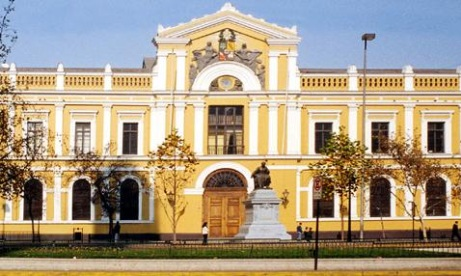
\includegraphics[width=\columnwidth]{./pictures/uchile.jpg}
\caption{Casa central de la Universidad de Chile}
\end{figure}

Es la más antigua del país (data de 1842) y una de las de mayor prestigio y tradición de América
Latina, como lo prueban múltiples reconocimientos nacionales e internacionales. En el plano
nacional, la Universidad de Chile recibe en términos relativos el mayor número de estudiantes con
los mejores puntajes de ingreso al sistema de educación superior, cuenta con un cuerpo académico
de excelencia, con una alta productividad en el campo científico y de la creación artística y cultural,
y está permanentemente vinculada a la reflexión y solución de los problemas nacionales.

Desde una perspectiva de regulación externa de la calidad, la Universidad participó en la
primera experiencia voluntaria de acreditación institucional en Chile (año 2004), habiendo sido
acreditada por la Comisión Nacional de Acreditación de Pregrado, (CNAP), en todas las áreas
consideradas (gestión estratégica, docencia de pregrado, investigación y creación, docencia de
postgrado, vinculación con el medio e infraestructura) y por el máximo período considerado
para estos efectos por el organismo citado (siete años). Durante el año 2011 la Universidad
se sometió a un segundo proceso de acreditación ante la Comisión Nacional de Acreditación
(CNA), manteniendo los siete años en todas las áreas consideradas. En lo internacional, mantiene
activas relaciones de intercambio científico, pedagógico, cultural y artístico con destacadas
universidades del continente americano, Europa y otros continentes y ocupa una alta posición
a nivel latinoamericano en rankings universitarios tales como el del Jiao Tong Institute de la
Universidad de Shanghai, y el del SCImago Research Group, de España.

Los orígenes de la Universidad de Chile se encuentran en las primeras universidades
conventuales que se fundan en el país durante el siglo XVII, en el período colonial, y que reciben
autorización real y pontificia para otorgar títulos de bachiller, licenciado, maestro y doctor en
filosofía y teología. Más tarde, en 1738, se crea una universidad real, docente y de claustro,
a la que se llama de San Felipe, en honor del rey Felipe V, con Facultades de leyes, teología,
medicina y matemáticas. Con motivo de la independencia del imperio español, esta institución
se adapta progresivamente a las nuevas circunstancias de la vida republicana y pasa a llamarse
Universidad del Estado de Chile, luego de la República de Chile, y finalmente, Universidad de
Chile. En 1842 se dicta una ley orgánica de acuerdo a la cual la Universidad de Chile recibe la
función de superintendencia de todos los niveles de la enseñanza del país. Asimismo, se le encarga
propagar la afición por los estudios superiores, promover la investigación y la divulgación científica
y literaria y servir de auxiliar a los trabajos de las diversas dependencias de la administración del
Estado. Cinco Facultades académicas forman entonces la universidad: Humanidades y Filosofía,
Ciencias Matemáticas y Físicas, Leyes y Ciencias Políticas, Medicina, y Teología. Estas Facultades
tenían una función eminentemente científica, puesto que la labor docente de la Universidad quedaba
radicada en el Instituto Nacional, fundado en 1811 e inaugurado el 10 de agosto de 1813. 
El 9 de enero de 1879 se dictó un nuevo estatuto
que transformó a la Universidad en una institución de finalidad docente.

En 1931 se dicta una nueva ley orgánica que consagra la doble función científica y docente de
la Universidad. A partir de entonces, y durante treinta años, se mantiene un crecimiento sostenido
de la Corporación. Crece el número de sus facultades e institutos, de sus centros de investigación
y de sus carreras y programas académicos. Las actividades de extensión reciben también un fuerte
impulso, creándose la Orquesta Sinfónica de Chile y el Teatro Experimental de la Universidad, en
1941; el Museo de Arte Popular Americano, en 1943; el Coro Universitario y el Ballet Nacional,
en 1945; y el Museo de Arte Contemporáneo, en 1947. Asimismo, se inicia la radiotelefonía
universitaria, y se realizan las Escuelas Internacionales de Temporada, que atraen a profesores y
estudiantes de todo el continente y llevan los contenidos de la ciencia y la cultura al gran público.
La realización de escuelas de temporada en provincia es el primer paso para la fundación de los
centros universitarios regionales, que luego se convierten en las distintas sedes que llega a tener
la Universidad en las principales ciudades del país. De estas sedes derivarán, más tarde, diversas
universidades autónomas.

Junto con formar profesionales y graduados, la Universidad de Chile ha cumplido a lo largo
de su historia una labor de primera importancia a nivel nacional, a la vez que se ha constituido en
uno de los principales centros de creación científica y artística y de irradiación cultural de América
Latina. La primera de las grandes tareas que emprende fue la organización de un sistema nacional
de educación, en el siglo XIX. En el siglo XX contribuye decisivamente a ampliar a todo el país
la cobertura de la atención primaria en salud, a superar el problema de la desnutrición infantil,
a la construcción de grandes obras de infraestructura productiva y energética, al estudio de los
materiales de construcción y al desarrollo de la ingeniería sismorresistente, con lo que se aminoran
en gran medida los efectos de los terremotos, y al desarrollo productivo exportador, especialmente
en las áreas silvoagropecuarias y minera, entre otras grandes tareas. En lo internacional, es
reconocida su acción en prácticamente todas las áreas.

En la actualidad, y para desarrollar sus actividades, la Universidad de Chile se organiza en
14 facultades, 4 institutos interdisciplinarios y tres centros. Las Facultades son: Arquitectura y
Urbanismo; Artes; Ciencias; Ciencias Agronómicas; Ciencias Físicas y Matemáticas; Ciencias
Forestales y Conservación de la Naturaleza; Ciencias Químicas y Farmacéuticas; Ciencias Sociales;
Ciencias Veterinarias y Pecuarias; Derecho; Economía y Negocios; Filosofía y Humanidades;
Medicina; y Odontología. Los Institutos son: Instituto de Asuntos Públicos (INAP); Instituto
de Estudios Internacionales (IEI); Instituto de Nutrición y Tecnología de los Alimentos (INTA)
e Instituto de Comunicación e Imagen (ICEI). Deben destacarse también el Hospital Clínico
José Joaquín Aguirre, el Liceo Experimental Manuel de Salas, una gran institucionalidad cultural
(Orquesta Sinfónica, Ballet Nacional, Coro de la Universidad de Chile, Teatro Nacional, Museo de
Arte Contemporáneo, Museo de Arte Popular Americano, Archivo Andrés Bello y otros), la Radio
de la Universidad de Chile y muchas otras instancias que se encuentran adscritas a Facultades e
Institutos.

La Universidad de Chile cuenta con una matrícula superior a 31 mil estudiantes de pregrado
distribuidos en 69 programas de estudio, los cuales incluyen 55 carreras profesionales y 
14 licenciaturas terminales. Además ofrece más de un centenar de programas de especialización en
diversas áreas.

En el período comprendido entre los años 2002 y 2017 la oferta de vacantes regulares (vía
PSU) ha aumentado desde los 4.000 a los 5.453 cupos anuales, y la oferta global de vacantes ha
crecido por sobre los 6.309 cupos anuales (para todas las vías de ingreso). En el año 2017, para un
total de 5.453 vacantes regulares, se registró un total de 17.910 postulaciones a la Universidad de
Chile.

% En el año <#ano_estadistica_matricula#>, el <.#porcentaje_matriculados_UCH#.>\% de los estudiantes que alcanzaron puntajes nacionales se matricularon
% en la Universidad de Chile; de igual forma, de entre todos los puntajes nacionales, el <.#porcentaje_colegio_municipal#.>\% de los
% provenientes de colegios municipales y el <.#porcentaje_colegio_subvencionados#.>\% de los provenientes de colegios subvencionados
% eligieron esta universidad para realizar sus estudios superiores, dando cuenta tanto de la percepción
% positiva que tienen los estudiantes y sus familias de la Universidad de Chile, como de la diversidad
% de éstos y la interacción de la Universidad con el medio social dado su carácter nacional y estatal.

Junto a este énfasis por la excelencia de los alumnos que ingresan, la Universidad de Chile se
esfuerza por fomentar la equidad. Concretamente, ha instituido la Beca de Equidad Universidad de
Chile que cubre la diferencia entre el arancel real y el arancel de referencia y que hasta ahora era
financiada por estos estudiantes a través de un crédito otorgado por el Fondo Solidario de Crédito
Universitario. Considerando que los estudiantes de los dos primeros quintiles de ingreso reciben
del MINEDUC una beca para financiar el arancel de referencia, la Beca de Equidad Universidad
de Chile significa, en los hechos, gratuidad de aranceles para los estudiantes más vulnerables.

% Dado que la Universidad de Chile es la institución de educación superior que matricula la
% mayor cantidad de alumnos dentro de los <.#mejores_puntajes_PSU#.> mejores puntajes en la PSU, es la que obtiene el
% mayor Aporte Fiscal Indirecto (AFI) del sistema educacional chileno.

El sistema de postgrado y postítulo de esta institución es el más grande y complejo del país,
compuesto por 38 programas de doctorado, 116 programas de magíster, 69 programas de título
profesional especialista y 13 cursos de especialización de postítulo, con cerca de 9.290 estudiantes,
todos estos valores vigentes hasta el año 2016.

A nivel de investigación, en el Concurso FONDECYT Regular en el período 2005-2012 la
Universidad de Chile se adjudicó 914 proyectos, lo que corresponde al 26\% del total nacional.
En el año 2012 este concurso adjudicó a la Universidad de Chile fondos por US\$37,8 millones
(\$17.766 millones equivalentes en pesos chilenos). A nivel del Concurso FONDECYT de Iniciación 2012, la
Universidad de Chile se adjudicó 51 de 293 proyectos (17,4\% del total) por un monto de \$3.041
millones, concentrando un 18,8\% del total de fondos asignados a nivel nacional (\$16.196 millones). En
cuanto al Concurso FONDECYT de Postdoctorado 2013, esta casa de estudios se adjudicó 61
de un total de 238 proyectos seleccionados (25,6\% del total) y \$3.779 millones de un total de
\$14.980 millones, correspondiente al 25,2\% del total de recursos asignados en este concurso.

Por otra parte es destacable mencionar que en el período 2010-2016 los académicos de la
Universidad de Chile tuvieron 12.037 publicaciones ISI, la mayor productividad académica a nivel nacional.

En la Universidad de Chile han sido formados la mayor parte de los Presidentes de la
República, incluyendo a Manuel Montt Torres, Federico Errázuriz Zañartu, Domingo Santa María,
Federico Errázuriz Echaurren, Germán Riesco, Pedro Montt, Ramón Barros Luco, Juan Luis
Sanfuentes, Arturo Alessandri Palma, Emiliano Figueroa, Juan Esteban Montero, Pedro Aguirre
Cerda, Gabriel González Videla, Jorge Alessandri Rodríguez, Salvador Allende Gossens, Patricio
Aylwin Azócar, Eduardo Frei Ruiz-Tagle, Ricardo Lagos Escobar y Michelle Bachelet Jeria. La
mayor parte de los ganadores de premios nacionales en las menciones de ciencias, humanidades y
artes son ex-alumnos de esta casa de estudios (180 Premios Nacionales).
%, que representan el <.#porcentaje_premios_UCH_del_total#.>\% del total).
Gabriela Mistral, receptora del Premio Nobel de Literatura (1945), y Pablo Neruda, 
receptor del Premio Nobel de Literatura (1971), fueron miembros de la Universidad de Chile.

Actualmente la Universidad se rige por un nuevo Estatuto que modifica el DFL N$^{\circ}$ 153 de
1981, dando lugar a una nueva institucionalidad: el Rector es la máxima autoridad unipersonal
y representante legal, quien es elegido por los pares académicos por un período de cuatro
años; el Senado Universitario, órgano colegiado con funciones normativas y de lineamientos
estratégicos, compuesto por 36 miembros (27 académicos, 7 estudiantes y 2 representantes del
personal de colaboración) elegidos por sus pares; el Consejo Universitario, órgano colegiado
de carácter ejecutivo, compuesto por el Rector quien lo preside, el Prorrector, los Decanos,
y dos miembros designados por el Presidente de la República; el Consejo de Evaluación, a
cargo de la superintendencia de los procesos de evaluación, calificación y autoevaluación a nivel
institucional e individual, integrado por 5 profesores de la más alta jerarquía académica, quienes
son propuestos por el Rector y nombrados por el Senado Universitario; el Prorrector, quien asesora
al Rector en materias de orden académico, económico-administrativo, jurídico y estudiantil, quien
lo reemplaza en caso de ausencia y coordina la 5 Vicerrectorías: (i) Asuntos Académicos, (ii)
Asuntos Económicos, (iii) Asuntos Estudiantiles y Comunitarios, (iv) Investigación y Desarrollo,
y (v) Extensión y Comunicaciones.

\section{Facultad de Ciencias Físicas y Matemáticas}

\begin{figure}[ht!]
\centering
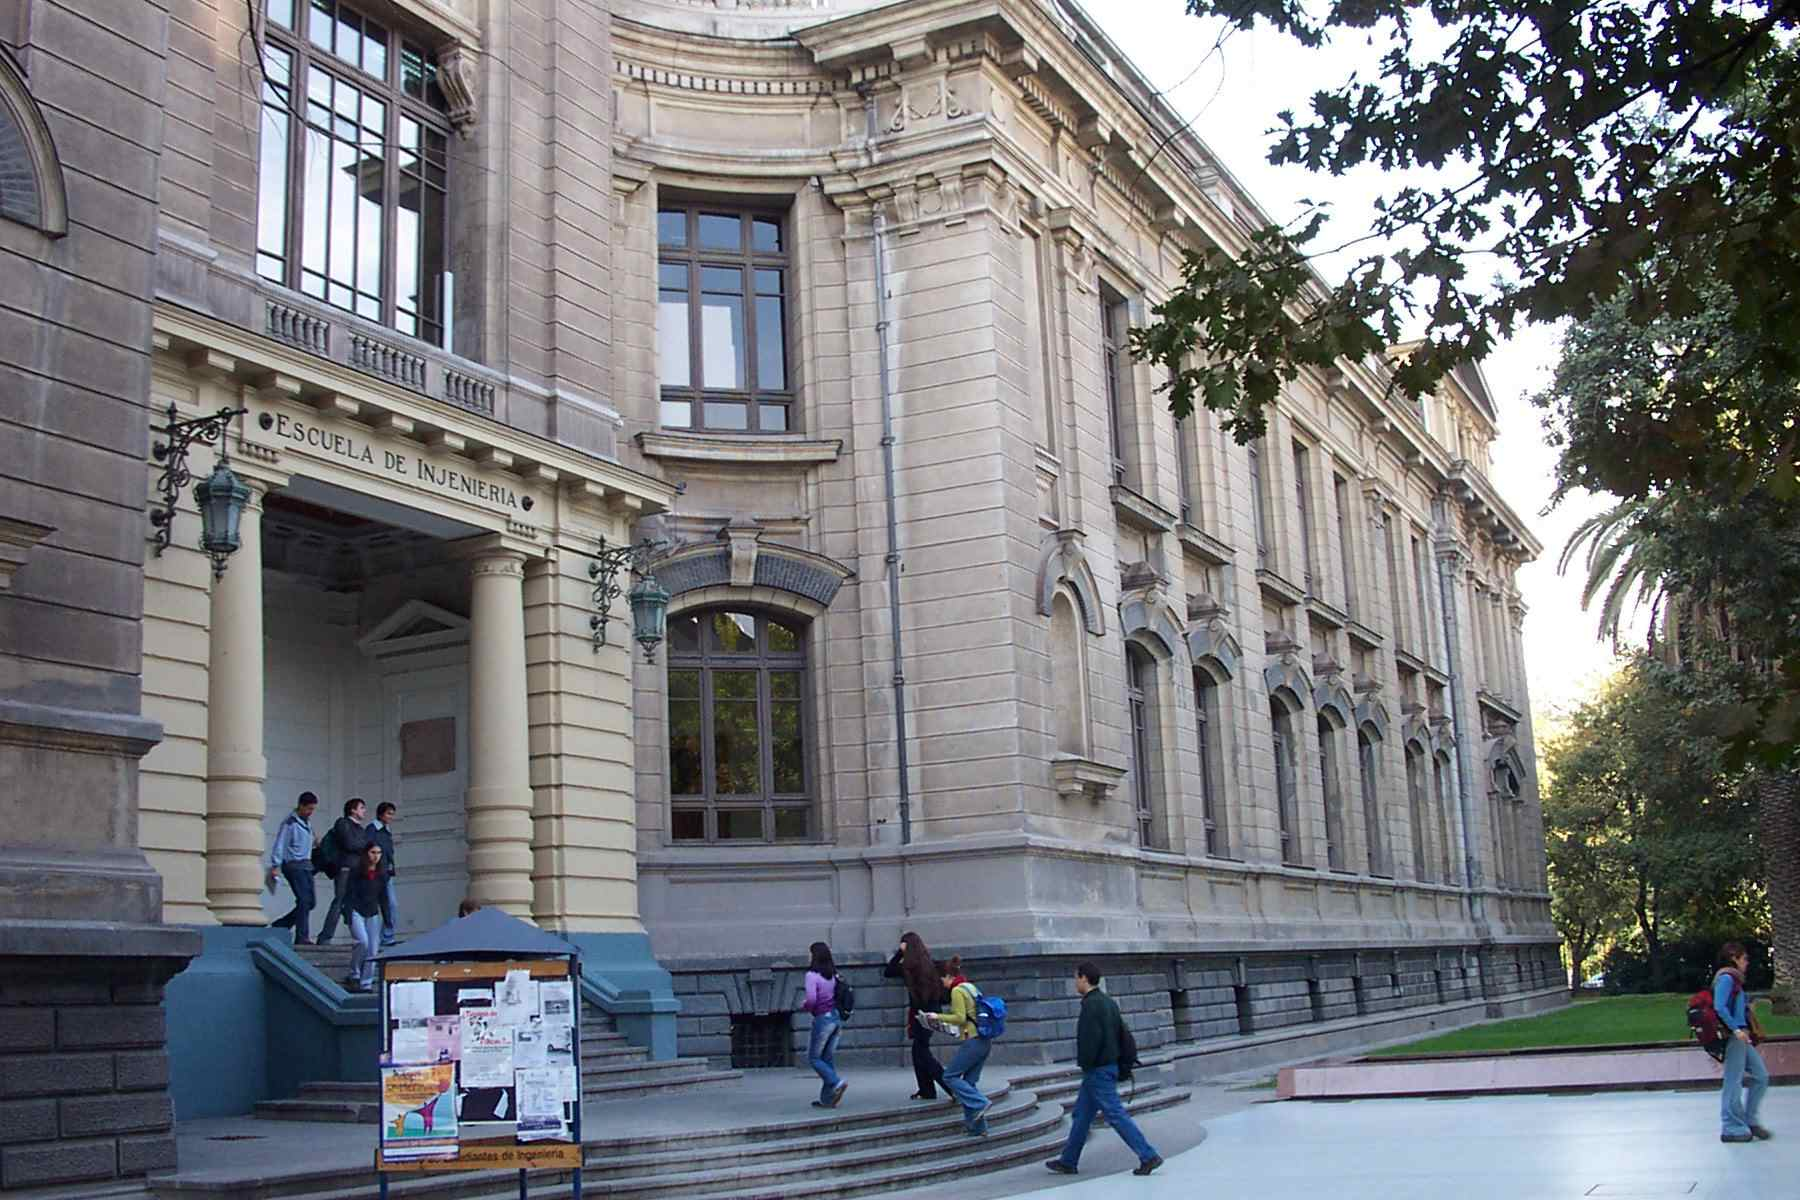
\includegraphics[width=\columnwidth]{./pictures/frontis.jpg}
\caption{Frontis de la entrada principal de la escuela de ingeniería}
\end{figure}

\subsection{Reseña Histórica}

La Facultad de Ciencias Físicas y Matemáticas (FCFM) es tan antigua como la propia Universidad
de Chile, ya que ambas se crearon en el año 1842, bajo el gobierno del Presidente Manuel Bulnes.

En ese entonces, Andrés Bello, quien fuera el primer Rector de la Universidad, le pidió al
ingeniero español, Andrés Antonio Gorbea que dirigiera esta nueva Facultad. Nueve años después,
en 1853, se organizó la enseñanza de la ingeniería propiamente tal impartiendo las especialidades de
Ingeniero Geógrafo, Ingeniero de Minas, Ingeniero de Puentes y Caminos, y también Arquitectura
(carrera que se independizó en 1946).

En 1911 comenzó la construcción de un nuevo edificio para la Facultad, ubicado en Santiago,
en la calle Benavente 850 -actual Beauchef-. La inauguración se realizó el 8 de abril de 1922, ante
la presencia de ministros de Estado, embajadores y el entonces Presidente de la República, Arturo
Alessandri Palma.

Con la creación de la Corporación de Fomento de la Producción (CORFO) en 1939 y de
grandes empresas públicas en los años 40, la Facultad debió adaptar las Escuelas de Ingeniería a la
nueva realidad tecnológica nacional.

Durante la segunda mitad del siglo XX, la FCFM continuó consolidando su liderazgo
en la formación de ingenieros y científicos, contribuyendo al desarrollo del país en áreas
como la electrificación, el agua potable, obras civiles de gran envergadura, el transporte y las
telecomunicaciones.

Como una forma de responder a los desafíos, a partir de los años 60 y hasta la década del 90
se empezaron a crear nuevas carreras como Ingeniería Civil en Matemáticas, en Computación, en
Materiales y, finalmente, en Biotecnología.

Con la llegada del siglo XXI, la Escuela de Ingeniería y Ciencias realizó cambios curriculares
con el objetivo de apoyar la innovación en la enseñanza y el aprendizaje. Para el diseño de estos
cambios, la Facultad adoptó metodologías originadas en el Massachusetts Institute of Technology
(MIT) que fueron incorporadas por las más prestigiosas escuelas de ingeniería del mundo. Dicho
método se conoce como iniciativa CDIO\footnote{Obtenido de \url{http://www.cdio.cl}}, denominada de esta manera para hacer énfasis en las
competencias de concebir, diseñar, implementar y operar sistemas de ingeniería.

En 2011 y como un reflejo de los 170 años de tradición y excelencia, la FCFM comenzó
la construcción del proyecto de infraestructura más importante desarrollado en los últimos 100
años, que se ubica en Beauchef 851, el que se describe en mayor detalle en la Sección \ref{infra_fcfm}
``Infraestructura de la FCFM''.

En la actualidad la Facultad presta importantes servicios de asesoría a organismos, empresas
y corporaciones estatales y privadas en todas las ramas de la ingeniería y la ciencia. Asimismo
continúa innovando y creando soluciones y requerimientos tecnológicos para enfrentar nuevos
escenarios.Dentro de esto, la facultad está trabajando en su nuevo Plan estratégico enmarcado en
el desarrollo del proyecto Ingeniería 2030 [\ref{fcfm_plan_2030}]. En el desarrollo del mismo se han realizado
seminarios, análisis y estudios tendientes a redefinir tanto las carreras como los programas de
postgrado y la articulación entre ellos.

\subsection{Estructura Orgánica de la FCFM}
\label{estruct_org_fcfm}

La estructura Orgánica de la FCFM que se ilustra en la Figura \ref{ograma_fcfm} está compuesta por el Decano,
Vicedecano, Consejo de Facultad, Dirección Académica y de Investigación, Dirección Económica
y Administrativa, División Jurídica, Escuela de Ingeniería y Ciencias, Escuela de Postgrado, 13
Departamentos, y Centros de Investigación y de Servicios. El Reglamento General de Facultades,
Decreto Universitario Exento N$\circ$ 906 de 27 de enero de 2009 [\ref{reg_gen_fac}], describe entre otros puntos
las funciones de las autoridades unipersonales, consejos y departamentos, como se resume a
continuación.

\begin{figure}[ht!]
\centering
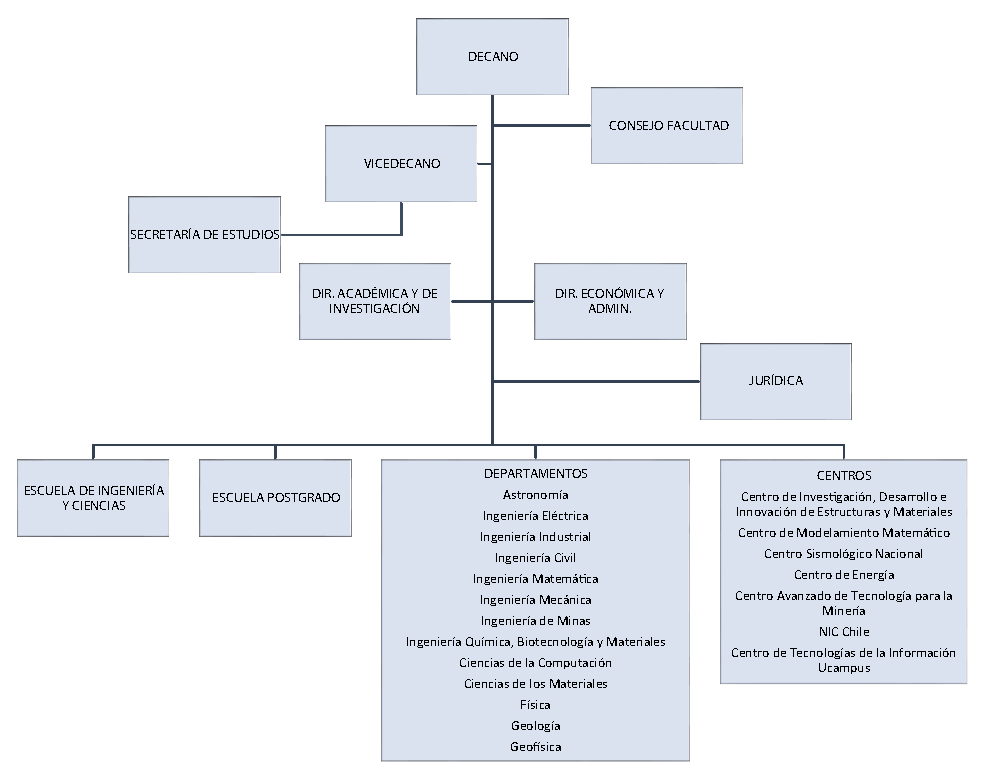
\includegraphics[width=\columnwidth]{./organigramas/organigrama_fcfm.eps}
\caption{Organigrama Facultad de Ciencias Físicas y Matemáticas de la Universidad de Chile}
\label{ograma_fcfm}
\end{figure}

El \textbf{Decano} es la máxima autoridad de la respectiva Facultad y le corresponde la dirección
de ésta, en el contexto de los lineamientos y estrategias emanados de los Órganos Superiores
de la Universidad, sin perjuicio de las atribuciones que el Estatuto Universitario le confiere al
Consejo de Facultad. El Decano debe ser Profesor Titular y es elegido por los académicos de la
Facultad. Dura cuatro años en el ejercicio de sus funciones, pudiendo ser elegido por un segundo
período consecutivo. Entre otras funciones, el Decano preside el Consejo de Facultad, propone
al Consejo de Facultad el presupuesto anual de financiamiento y darle cuenta de su ejecución,
propone al Rector, para su nombramiento, las personas que ocuparán los cargos o desempeñarán
las funciones, según sea el caso, de Vicedecano, Directores de Escuelas, Centros y direcciones de
asesoría integral, aprobados por el Consejo de Facultad; ejerce la potestad disciplinaria sobre las
personas que integren la Facultad, conforme a la normativa vigente; autoriza y ejecuta los gastos
que sean necesarios para el buen funcionamiento académico y administrativo de la Facultad.

El \textbf{Vicedecano} es el Ministro de Fe de la Facultad y el subrogante legal del Decano; dependen
de él los organismos de apoyo y asesoría integral establecidos en el artículo 4$^{\circ}$ y le corresponde
desempeñar las demás funciones que el Decano expresamente le delegue.

El \textbf{Consejo de Facultad} es presidido por el Decano, al que le corresponderá definir las
políticas de desarrollo académico e institucional en el contexto de los lineamientos y estrategias
emanados del Senado Universitario, con las atribuciones, funciones y responsabilidad que señala la
reglamentación vigente. Además del Decano, que lo preside, el Consejo de Facultad está integrado
por los Directores de los Departamento y Escuelas. Corresponde igualmente que lo integren los
Directores de los Institutos de Facultad y los Directores de aquellos Centros que tengan carácter de
permanentes. También lo integran académicos elegidos (6 en el caso de la FCFM), quienes duran
dos años en sus funciones, pudiendo ser elegidos sólo por un segundo período consecutivo. Asisten
al Consejo, con derecho a voz, representantes de las organizaciones gremiales, más representativas
de académicos, estudiantes y personal de colaboración de la correspondiente Facultad, nombrados
mediante los procedimientos que dichas organizaciones acuerden. También asiste el Vicedecano
en calidad de Secretario y Ministro de Fe, solo con derecho a voz. Las atribuciones del Consejo de
Facultad que están descritas en el Reglamento General de Facultades son, entre otras:

\begin{enumerate}
\item Aprobar las propuestas de políticas de admisión de alumnos de pre y postgrado propuestas
por las respectivas Escuelas para ser presentadas al Rector.
\item Aprobar el presupuesto anual de Facultad propuesto por el Decano.
\item Aprobar el Informe semestral y cuenta anual presentada por el Decano.
\end{enumerate}

La \textbf{Secretaría de Estudios} es una unidad dependiente del Vicedecano, que se encarga de
cautelar el cumplimiento de la normativa vigente en el desarrollo de los programas, siendo
responsable de gestionar el proceso de graduación y titulación de los estudiantes de Pregrado y
Postgrado, certificar sus situaciones académicas, y gestionar el proceso de matrícula.

La \textbf{Dirección Económica y Administrativa (DEA)} tiene a su cargo la gestión financiera de
la Facultad. Cada Unidad dispone de una organización administrativa local, de manera que la
gestión financiera se realiza esencialmente en forma descentralizada, pero bajo control contable
y del cumplimiento de la normativa vigente de la Dirección Económica y Administrativa. El
organigrama de esta Dirección y su relación con los Departamentos es el que se muestra en la
Figura \ref{ograma_dea_fcfm}.

\begin{figure}[ht!]
\centering
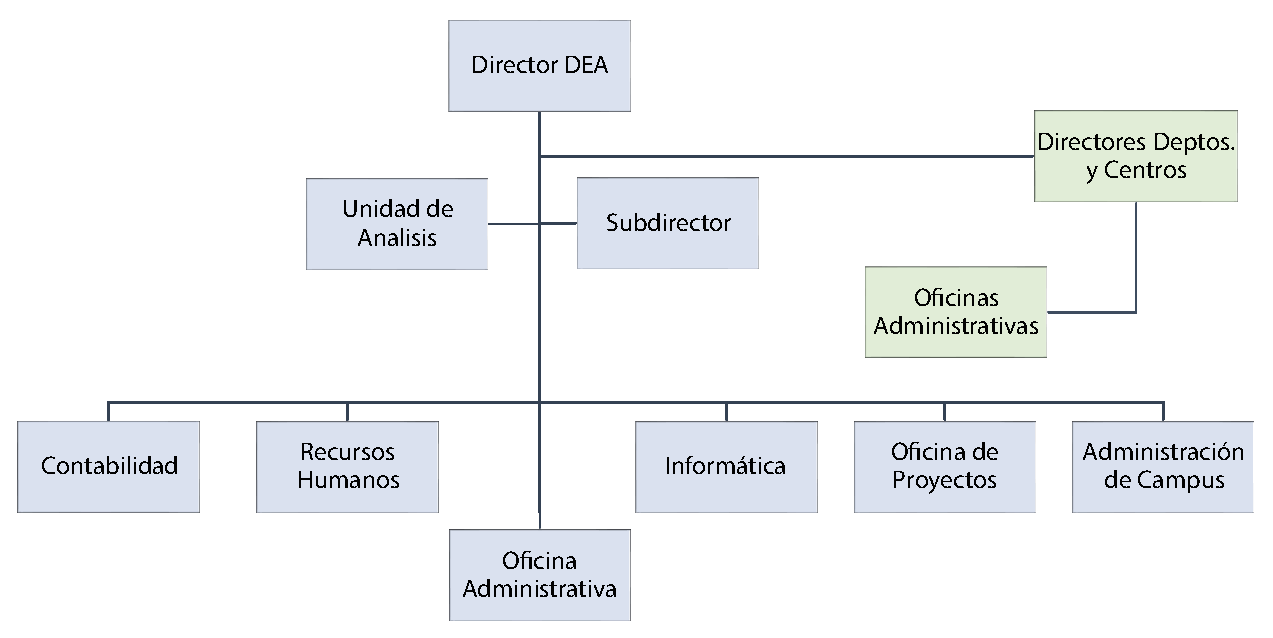
\includegraphics[width=\columnwidth]{./organigramas/organigrama_dea_fcfm.eps}
\caption{Organigrama de la Dirección Económica y Administrativa de la FCFM}
\label{ograma_dea_fcfm}
\end{figure}

La \textbf{Dirección Académica y de Investigación} tiene como misión contribuir, incentivar y
apoyar el desarrollo académico y la labor de investigación científica, tecnológica y de I\&D
en y entre las unidades académicas. Su propósito es, además, fomentar las actividades
multidisciplinarias. Entre sus prioridades institucionales se cuentan:

\begin{itemize}
\item Reforzar y transparentar la sistematización de la información en el área de investigación y
desarrollo facilitando y potenciando enfoques multidisciplinarios.
\item Apoyar a asesorar en el desarrollo académico a los Departamentos.
\item Contribuir a mantener el liderazgo en ciencia y tecnología, enfatizando la investigación como
parte fundamental de la labor académica.
\end{itemize}

La \textbf{Escuela de Ingeniería y Ciencias} tiene a su cargo la administración central de los planes de
estudio de pregrado y la coordinación de la enseñanza que imparten los departamentos académicos
de la Facultad.

La \textbf{Escuela de Postgrado} está encargada de organizar, administrar y coordinar los 23
programas de Magíster, 12 programas de Doctorado y los Diplomas de Postítulo ofrecidos por
la Facultad.

Los \textbf{Departamentos} que conforman la FCFM corresponden a:

\begin{enumerate}
\item Astronomía
\item Ciencia de los Materiales
\item Ciencias de la Computación
\item Física
\item Geología
\item Ingeniería Civil
\item Ingeniería de Minas
\item Ingeniería Eléctrica
\item Ingeniería Matemática
\item Ingeniería Mecánica
\item Ingeniería Química y Biotecnología
\end{enumerate}

La FCFM actualmente cuenta con 11 centros de investigación, en los que están involucrados
% más del <.#porcentaje_JC_en_CI_FCFM#.>\% del cuerpo académico de jornada completa, 
30 post-doctorantes.
% y <.#doctorado_en_CI_FCFM#.> tesistas de doctorado. 
Cada uno es líder en su disciplina en el país y en ellos se realiza la mayor actividad
de vinculación con el sector productivo y la sociedad, con énfasis en la creación de conocimiento,
desarrollo y transferencia tecnológica. Estos son:

\begin{itemize}
\item Centro de Modelamiento Matemático (CMM)
\item Centro Avanzado de Tecnología para la Minería (AMTC)
\item Centro de Excelencia en Geotermia de Los Andes (CEGA)
\item Instituto Sistemas Complejos de Ingeniería (ISCI)
\item Centro de Investigaciones en Energía Solar (SERC-Chile)
\item Centro de Ciencia del Clima y la Resiliencia (CR2)
\item Centro de Astrofísica y Tecnologías Afines (CATA)
\item Instituto Milenio de Astrofísica (MAS)
\item Centro de Biotecnología y Bioingeniería
\item Centro de Energía (CE)
\item Instituto Milenio para la Investigación de las Imperfecciones de Mercado y Política Pública (MIPP)
\end{itemize}

\subsection{Contexto de la FCFM}

\subsubsection{Oferta de títulos y grados de la FCFM}

La FCFM cuenta con una amplia oferta de título y grados. En pregrado, se ofrecen 10 carreras
profesionales que corresponden a Ingeniería Civil, Ingeniería Civil de Minas, Ingeniería Civil
en Biotecnología, Ingeniería Civil en Computación, Ingeniería Civil Eléctrica, Ingeniería Civil
Industrial, Ingeniería Civil Matemática, Ingeniería Civil Mecánica, Ingeniería Civil Química y
Geología; y 3 Licenciaturas en Astronomía, Física y Geofísica.

Además, cuenta con 23 programas de magíster en Astronomía, Computación, Física,
Geofísica, Geología, Ingeniería Eléctrica, Ingeniería Geotécnica, Ingeniería Química, Ingeniería
Sísmica, Ingeniería Mecánica, Metalurgia Extractiva, Recursos y Medioambiente Hídrico,
Transporte, Economía Aplicada, Gestión de Operaciones, Gestión y Dirección de Empresas,
Gestión y Políticas Públicas, Gestión para la Globalización, Ingeniería de Negocios con
Tecnologías de la Información, Ingeniería en Redes de Comunicaciones, Meteorología y
Climatología, Minería, Tecnologías de la Información.

Por último, la FCFM ofrece 12 programas de doctorado correspondientes a Astronomía,
Computación, Física, Geología, Ciencia de los Materiales, Fluidodinámica, Ingeniería Química,
Modelación Matemática, Ingeniería de Minas, Ingeniería Eléctrica, Sistemas de Ingeniería.

\subsubsection{Infraestructura de la FCFM} \label{infra_fcfm}

Campus Beauchef El Campus Beauchef de la Universidad de Chile alberga los edificios,
laboratorios, aulas, infraestructura deportiva y áreas verdes de la FCFM. Ubicado en la comuna
de Santiago, sus dependencias comprenden dos manzanas, encuadradas entre las calles Blanco
Encalada, Plaza Ercilla, Tupper y Club Hípico, separadas entre sí por la calle Beauchef, donde se
encuentra su entrada principal en Beauchef 850. El mapa del Campus Beauchef se muestra en la
Figura \ref{map_fcfm}.

\begin{figure}[ht!]
\centering
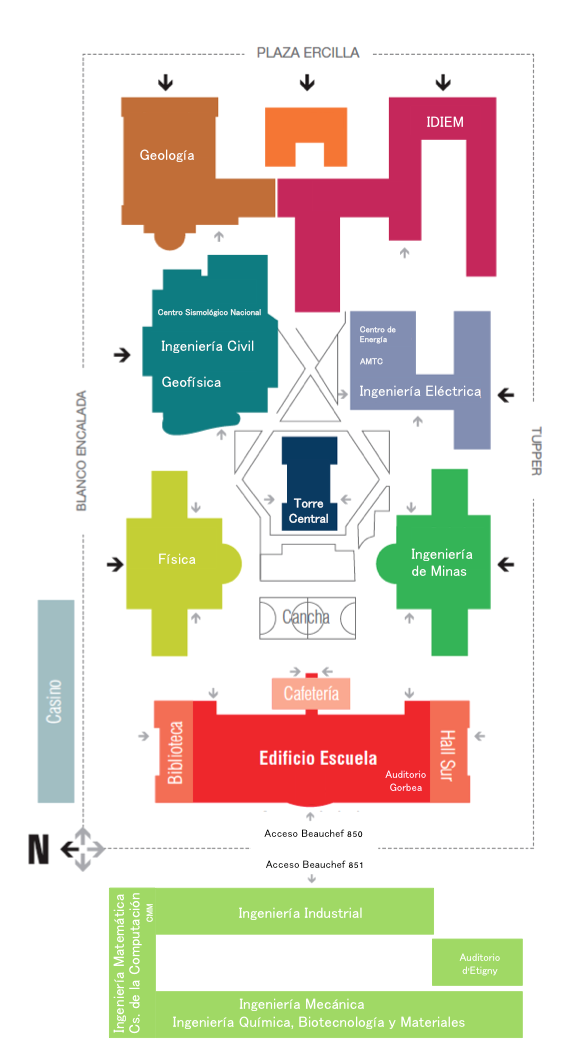
\includegraphics[width=0.94\columnwidth]{./pictures/mapa_fcfm.jpg}
\caption{Mapa Campus Beauchef}
\label{map_fcfm}
\end{figure}

El Campus Beauchef cuenta con 24 edificios, que suman 80.000 m$^2$ de superficie construida,
sobre un terreno de 36.000 m$^2$ donde se albergan más de 85 laboratorios con fines docentes y de
investigación.

La FCFM posee numerosos jardines que incluyen decenas de valiosas especies nativas y
foráneas, las cuales constituyen un interesante jardín botánico que adorna y da vida al Campus
Beauchef.

Los alumnos cuentan con una amplia sala con computadores centralizada, a la que se suman las
salas de computación disponibles en los Departamentos de Computación, Química y Biotecnología,
Mecánica, Civil, Eléctrica, Matemática, Geofísica, Geología y Astronomía.
Además, la Facultad cuenta con redes de comunicación de alta velocidad: fibra óptica y WiFi,
a disposición de todos los estudiantes, con acceso libre a Internet.

La FCFM posee más de 70 salas de clases, auditorios implementados con sofisticados equipos
para video conferencia, además de salas multimedia, y cómodas salas de estudio. En marzo de
2014 se instalaron modernas pizarras de acero porcelanizado, que es el material más moderno y
efectivo que existe en la actualidad para este tipo de trabajos, en 13 salas de Beauchef 850 y 8 salas
de Beauchef 851. Éstas fueron traídas desde EE.UU. y buscan darle más versatilidad a la enseñanza
en la Facultad.
La FCFM cuenta con un Sistema de Bibliotecas formado por la Biblioteca Central y
7 Bibliotecas Departamentales (Astronomía, Civil, Física, Geofísica, Geología, Industrias y
Matemáticas), con las más modernas tecnologías que permiten el acceso local y remoto a las
colecciones. Los otros Departamentos (Eléctrica, Mecánica, Química y Biotecnología, Minas)
decidieron tener un manejo centralizado de los volúmenes a través de la biblioteca central. El
sistema cuenta con un acervo bibliográfico de más de 185.000 volúmenes de libros, y acceso en
línea a: más de 52.000 revistas electrónicas y 150 bases de datos bibliográficas multidisciplinarias
y especializadas (con acceso a más de 2,2 millones de publicaciones en permanente actualización).
Para la realización de actividades deportivas la FCFM cuenta con múltiples espacios, que
corresponden a:

\begin{itemize}
\item Multicancha: Se encuentra al aire libre en el patio principal del campus Beauchef. En ella se
practica baby fútbol, voleibol y otros deportes en equipo.
\item Gimnasio, hubicado en Beauchef 851, está completamente
equipado con piscina, canchas de baloncesto, voleibol, tennis, racquetball y 
salas para actividades de musculación, preparación física, gimnasia aeróbica y taichí,
entre otras. 
\item Gimnasio Polideportivo Domeyko: Se emplaza en Almirante Latorre 730 y es un amplio
espacio que cuenta con equipamiento deportivo de primer nivel. Allí se practican deportes
como básquetbol, voleibol, tenis de mesa, gimnasia artística, judo, kárate y taekwondo, entre
otros.
\end{itemize}

Además, la Facultad tiene convenios para utilizar las instalaciones del Club de Tenis Santiago,
el Estadio Macul, el Estadio de Fútbol del Banco del Estado, la Piscina de la Universidad de Chile,
y otras dependencias deportivas de nuestra institución como el Refugio Cordillerano de Farellones.
El campus es complementado por instalaciones que lo rodean como el casino, ubicado en Blanco
Encalada 2085, y el Centro de Estudiantes de Ingeniería, en Tupper 2140.
La Facultad, además, cuenta con dependencias fuera del campus Beauchef, incluyendo el
Departamento de Ingeniería Industrial, ubicado en Avda. República 701; los laboratorios de
Ingeniería Mecánica, en Blanco Encalada 2743; y el Departamento de Astronomía, en el cerro
Calán, comuna de Las Condes, a los pies de la cordillera de Los Andes. Actualmente se encuentran
plenamente operativas las instalaciones del campus Beauchef 851.

Beauchef 851 es la más extensa ampliación en infraestructura del campus de la
FCFM desde su inauguración, hace más de un siglo. Este conjunto de edificaciones, emplazado
en la manzana poniente del campus, aumentó en un 50\% la infraestructura actual, y marca un hito
arquitectónico entre los espacios destinados a educación superior en Chile (ver Figura \ref{b851}). La
edificación cuenta con cerca de 50.000 m$^2$ construidos, distribuidos en siete pisos sobre superficie
y seis subterráneos. Allí se ubican salas de clases, laboratorios, oficinas, auditorios, espacios
deportivos y de recreación, y estacionamientos.

\begin{figure}[ht!]
\centering
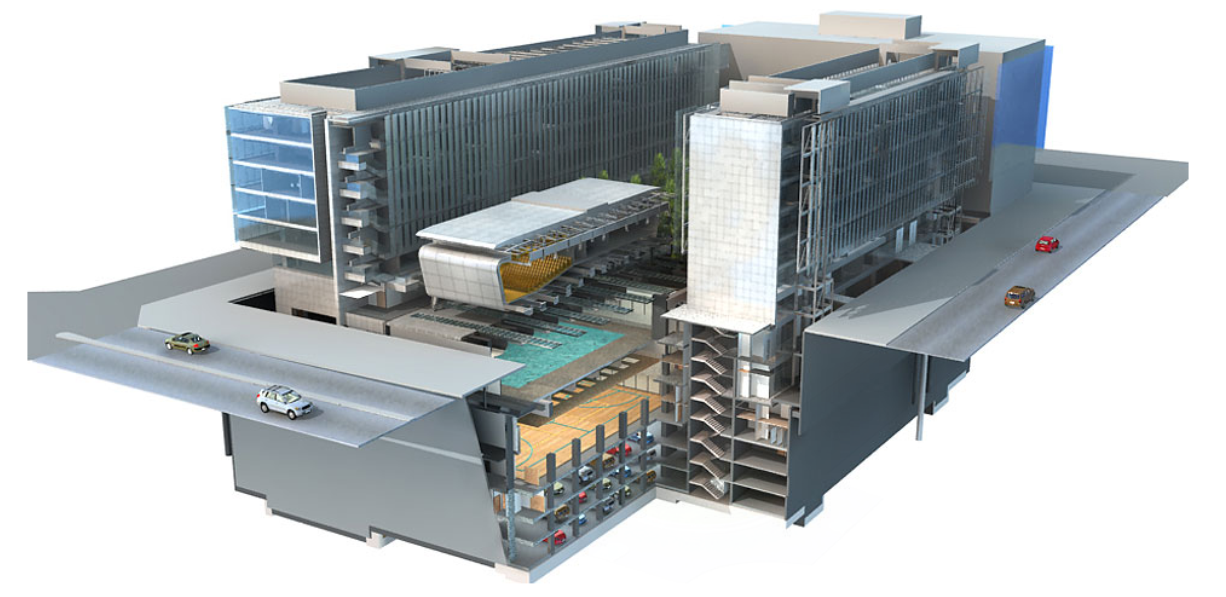
\includegraphics[width=\columnwidth]{./pictures/beauchef851.png}
\caption{Modelo tridimensional de Beauchef 851}
\label{b851}
\end{figure}

Uno de los sellos distintivos de Beauchef 851 es la eficiencia energética incorporada en su
diseño, construcción y operación, lo que permitirá certificarlo bajo los exigentes estándares LEED
ante el Consejo de Edificios Verdes de Estados Unidos (USGBC).

\subsubsection{Planta Docente de la FCFM}

La FCFM cuenta con 225 académicos de jornada completa (septiembre 2014) dedicados a la
investigación y/o innovación tecnológica para Chile y el mundo. También cuenta con más de
200 profesores con jornada parcial en contacto permanente con la industria.

En cuanto a los académicos de jornada completa, el 90\% de éstos posee el título de doctor
en el área donde hace clases e investigación y muchas veces incluyen a estudiantes dentro de sus
investigaciones, lo que aporta enormemente a su formación.
Entre el total de académicos – tanto jornada completa como parcial - casi el 70\% posee algún
tipo de postgrado. Además, la FCFM cuenta con más de 70 investigadores de postdoctorado. Éstos
y otros números se pueden ver en la Tabla \ref{jor_vs_grados}.

% Tabla 1.1
\begin{table}[ht!]
\centering
\caption{Número de docentes según jornada de contrato y grado académico.}
\label{jor_vs_grados}
\begin{tabular}{llllll}
\hline
Profesor         & \shortstack{Licenciados \\ o Titulados} 	& Con Magíster & Con Doctorado & Total & Con Postgrado \\ \hline \hline
Jornada Completa & 15	& 6 & 204 & 225 & 93,3\%          \\ \hline
Media Jornada    & 1 & 0 & 1 & 2 & 50\%          \\ \hline
Por Hora         & 123 & 39 & 61 & 223 & 44,8\%          \\ \hline
\textbf{Total}   & 139 & 45 & 266 & 450 & 69,1\%          \\ \hline
\end{tabular}
\end{table}

Los docentes del Plan Común, en gran parte, están adscritos a Departamentos de la FCFM,
principalmente a los Departamentos de Ingeniería Matemática, Física, Ingeniería Industrial,
Ciencias de la Computación y Ciencias de los Materiales. En el año 2013, de los 99 docentes
del Plan Común, 82 tenían grado de Doctor, 5 Magíster y 12 titulados y licenciados. De ese total
de docentes, 77 estaban a jornada completa y 22 eran contratados por hora.
Los académicos e investigadores de la FCFM publicaron 2.257 artículos científicos en revistas
ISI durante el año 2016. 
% El <.#porcentaje_con_factor_impacto_Q1#.>\% de las publicaciones ISI originadas en la Facultad tienen un factor de impacto Q1.

Desde el punto de vista de la jerarquización académica, la planta docente de la Facultad se
encuentra compuesta como se muestra en la Tabla \ref{jer_vs_grado}.

% Tabla 1.2
\begin{table}[hb!]
\centering
\caption{Número de docentes según jerarquía y grado académico.}
\label{jer_vs_grado}
\begin{tabular}{llllll}
\hline
Profesor        & \shortstack{Licenciados \\ o Titulados} & Con Magíster & Con Doctorado & Total & Con Postgrado \\ \hline \hline
Prof. Titular   & 17    & 4    & 70    & 91    & 81,3\%          \\ \hline
Prof. Asociado  & 20    & 4    & 77    & 101    & 80,2\%          \\ \hline
Prof. Asistente & 10    & 5    & 91    & 106    & 90,6\%          \\ \hline
Prof. Adjunto   & 40    & 12    & 17    & 69    & 42\%          \\ \hline
Inst. Adjunto   & 42    & 19    & 6    & 67    & 37,3\%          \\ \hline
Instructor      & 6    & 1    & 4    & 11    & 45,5\%          \\ \hline
Ayudante        & 4    & 0    & 0    & 4    & 0\%           \\ \hline
No Evaluado     & 0    & 0    & 1    & 1    & 100\%         \\ \hline
\textbf{Total}  & 139 & 45 & 266 & 450 & 69,1\%          \\ \hline
\end{tabular}
\end{table}

Otro factor importante en la formación de ingenieros y científicos es la presencia tanto de
académicos jóvenes como aquellos con más experiencia. Por esto, en la FCFM se han contratado
a cada vez más académicos jóvenes y esto puede demostrarse con la información entregada en la
Figura \ref{etario}, donde cerca del 46,8\% de los académicos son menores de 50 años.

\begin{figure}[ht!]
\centering
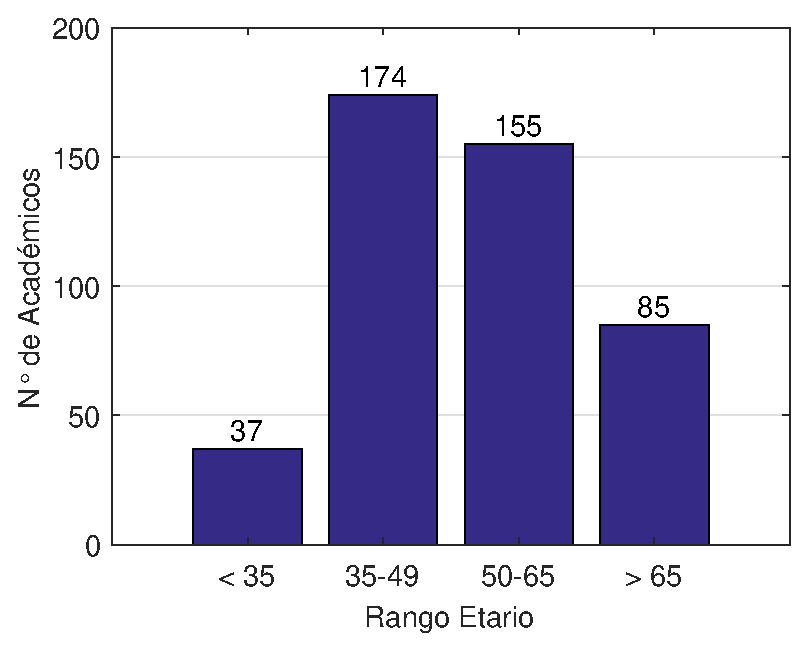
\includegraphics[width=0.65\columnwidth]{./pictures/etario.eps}
\caption{Rango etario de académicos de la FCFM.}
\label{etario}
\end{figure}

\subsubsection{Perfil de los estudiantes de la FCFM}\label{prefil_fcfm}

A la Escuela de Ingeniería y Ciencias ingresaron 695 alumnos (ingreso regular) el año 2014. Así,
los jóvenes que se unen a esta Facultad se incorporan a una institución viva, que se actualiza y
renueva constantemente, difundiendo conocimientos y estableciendo estándares para la docencia
y la investigación en ingeniería y ciencias afines, formación que es reconocida a nivel nacional e
internacional.

%La principal vía de admisión es a través de la Prueba de Selección Universitaria (PSU) según
%las ponderaciones indicadas en la Tabla \ref{psu}.

%\begin{table}[ht]
%\centering
%\caption{Ponderación puntajes de ingreso a la FCFM.}
%\label{psu}
%\begin{tabular}{lll}
%\hline
%                                  & 2003-2011 & 2012-presente \\ \hline \hline
%Prueba de Matemáticas             & 50\%      & 45\%          \\ \hline
%Prueba de Lenguaje y Comunicación & 10\%      & 10\%          \\ \hline
%Prueba de Ciencias                & 20\%      & 15\%          \\ \hline
%Notas de Enseñanza Media          & 20\%      & 10\%          \\ \hline
%Ranking de Egreso                 & 0\%       & 20\%          \\ \hline
%\end{tabular}
%\end{table}

%Inicialmente se ingresa a un programa de Plan Común. Este es un período de estudios que dura
%4 semestres y que entrega una sólida base en física y matemática, necesaria para desenvolverse en
%el mundo tecnológico de hoy. La ventaja de esta modalidad, utilizada en las universidades más
%prestigiosas, es que posterga la elección de la carrera a los recién egresados de Enseñanza Media,
%hasta una etapa en que los intereses de los alumnos están más definidos.

%Procedencia de los alumnos La Universidad de Chile se caracteriza por la diversidad de sus
%alumnos, y en la FCFM no es la excepción. La Tabla \ref{ingreso_fcfm} indica la procedencia de los alumnos que
%ingresan a Plan Común según tipo de establecimiento, donde se puede apreciar que más de la mitad
%de los alumnos provienen de establecimientos municipales o subvencionados. 

%\begin{table}[!ht]
%\centering
%\caption{Ingreso a la FCFM por tipo de establecimiento.}
%\label{ingreso_fcfm}
%\begin{tabular}{llll}
%\hline
%Año                                                                                & 2011 & 2012 & 2013 \\ \hline \hline
%\begin{tabular}[c]{@{}l@{}}N$\circ$ de alumnos de primer año que provienen \\ de establecimientos municipales\end{tabular}          & 189  & 154  & %152  \\ \hline
%\begin{tabular}[c]{@{}l@{}}N$\circ$ de alumnos de primer año que provienen \\ de establecimientos subvencionados\end{tabular}       & 182  & 200  & %220  \\ \hline
%\begin{tabular}[c]{@{}l@{}}N$\circ$ de alumnos de primer año que provienen \\ de establecimientos particulares pagados\end{tabular} & 357  & 332  & %312  \\ \hline
%Sin información                                                                    & 0    & 2    & 5    \\ \hline
%\textbf{Total}                                                                     & 728  & 688  & 689  \\ \hline
%\end{tabular}
%\end{table}


Los estudiantes que
ingresan a la FCFM son parte del 3\% superior de rendimiento en la PSU. El puntaje de cierre de
ingreso se encuentra por sobre los 712.3 puntos, mientras que los máximos puntajes ingresados llegan
hasta los 840.1 puntos. La Figura \ref{puntajes_psu} muestran los puntajes PSU máximo, mínimo y promedio de
ingreso al Plan Común en los últimos años.

\begin{figure}[ht!]
\centering
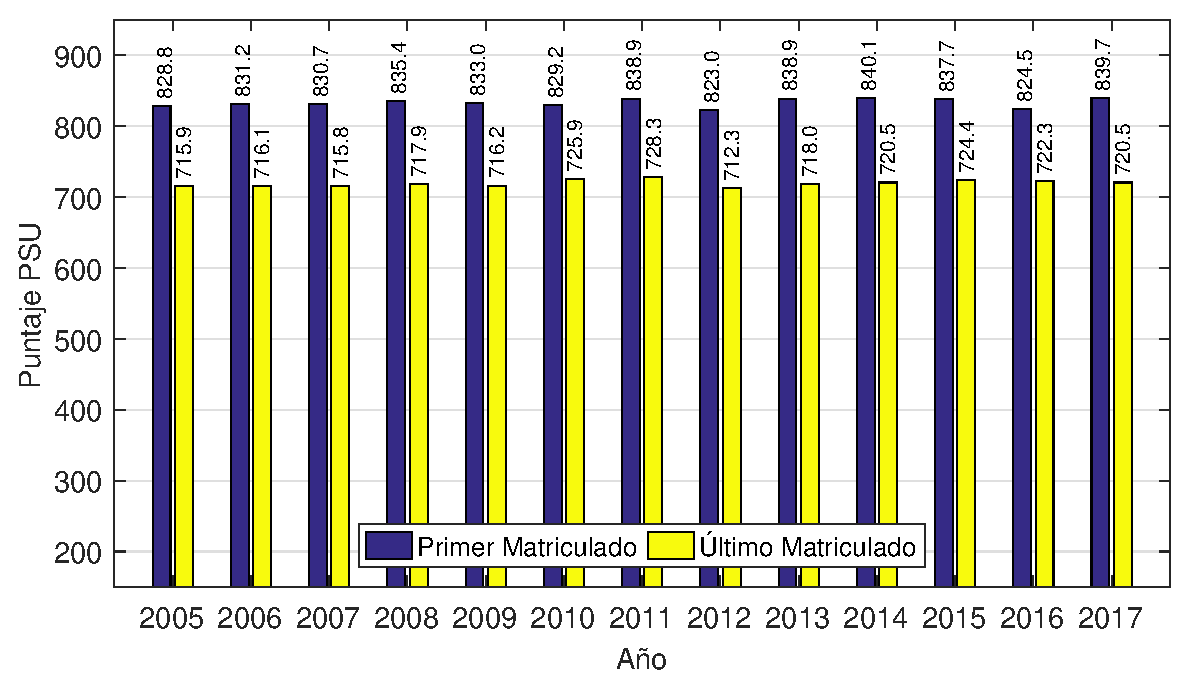
\includegraphics[width=\columnwidth]{./pictures/puntajes_psu.eps}
\caption{Puntajes de Ingreso a la FCFM.}
\label{puntajes_psu}
\end{figure}

%Como se observa en la Tabla \ref{ingreso_regiones}, a la FCFM ingresan alumnos provenientes de todas las
%regiones del país, confiando en que recibirán la mejor formación en ingeniería y ciencias. Si bien
%la mayor parte reside en la Región Metropolitana, alrededor de un <.#ingreso_otras_regiones_FCFM#.>\% de los alumnos son de otras
%regiones, siendo la <@regiones_mas_representadas@> región las más representadas.

%\begin{table}[!ht]
%\centering
%\caption{Procedencia de alumnos por regiones (2012).}
%\label{ingreso_regiones}
%\begin{tabular}{lccccccc}
%\hline
%Región                   & I   & II  & III  & IV  & V    & VI   & VII  \\ \hline \hline
%Ingreso               & <.#in_reg(1)#.>\% & <.#in_reg(2)#.>\% & <.#in_reg(3)#.>\%    & <.#in_reg(4)#.>\% & <.#in_reg(5)#.>\%  & <.#in_reg(6)#.>\%  %& <.#in_reg(7)#.>\%  \\[0.3cm] \hline
%\multicolumn{1}{r}{VIII} & IX  & X   & XI   & XII & RM   & XIV  & XV   \\ \hline \hline
%\multicolumn{1}{r}{<.#in_reg(8)#.>\%}  & <.#in_reg(9)#.>\% & <.#in_reg(10)#.>\% & <.#in_reg(11)#.>\% & <.#in_reg(12)#.>\%   & <.#in_reg(13)#.>\% & %<.#in_reg(14)#.>\% & <.#in_reg(15)#.>\% \\ \hline
%\end{tabular}
%\end{table}


%Desde hace algunos años, el porcentaje de mujeres en la Facultad se ha mantenido estable
%alrededor del 20\% (ver Tabla \ref{infreso_genero}), cifra muy superior a Facultades de Ingeniería de otras
%Universidades, en las que el número de mujeres es muy reducido. Desde 2014, se comenzó a
%implementar el Programa de Ingreso Prioritario de Equidad de Género, que considera el aumento
%de 40 cupos especiales para mujeres que queden en lista de espera, y así mejorar su participación
%en la comunidad de la FCFM.

%\begin{table}[ht]
%\centering
%\caption{Procedencia de alumnos por género.}
%\label{infreso_genero}
%\begin{tabular}{lccccccccc}
%\hline
%Año     & <#ano_in(1)#> & <#ano_in(2)#> & <#ano_in(3)#> & <#ano_in(4)#> & <#ano_in(5)#> & <#ano_in(6)#> & <#ano_in(7)#> & <#ano_in(8)#> & %<#ano_in(9)#>   \\ \hline \hline
%Mujeres & <.#in_muj(1)#.>\% & <.#in_muj(2)#.>\% & <.#in_muj(3)#.>\% & <.#in_muj(4)#.>\% & <.#in_muj(5)#.>\% & <.#in_muj(6)#.>\% & <.#in_muj(7)#.>\% %& <.#in_muj(8)#.>\% & <.#in_muj(9)#.>\% \\ \hline
%Hombres & <.#in_hom(1)#.>\% & <.#in_hom(2)#.>\% & <.#in_hom(3)#.>\% & <.#in_hom(4)#.>\% & <.#in_hom(5)#.>\% & <.#in_hom(6)#.>\% & <.#in_hom(7)#.>\% %& <.#in_hom(8)#.>\% & <.#in_hom(9)#.>\% \\ \hline
%\end{tabular}
%\end{table}

\subsection{Descripción de la unidad y su proceso de enseñanza-aprendizaje}

La FCFM comenzó hace más de diez años, de forma pionera, una revisión profunda de sus
currículos de carreras y programas, de los contenidos de sus asignaturas y de sus métodos docentes.
Este rediseño se ha enmarcado dentro del modelo desarrollado por la Iniciativa CDIO (Concibe,
Diseña, Implementa y Opera), que agrupa alrededor de un centenar de escuelas de ingeniería en el
mundo, que trabajan en conjunto para mejorar su enseñanza. La Escuela de Ingeniería y Ciencias
de la FCFM es responsable de liderar la región latinoamericana de CDIO.

La experiencia adquirida en la aplicación del nuevo plan de estudios, iniciado en 2007, ha
demostrado la importancia de que los cambios curriculares vayan acompañados de cambios en las
metodologías de enseñanza-aprendizaje, que coloquen al estudiante al centro del proceso educativo.
Esto coincide con la disponibilidad creciente de tecnología, tanto para el profesor como para los
alumnos. A menudo, esta tecnología ha venido a reforzar los métodos expositivos tradicionales, que
mantienen al alumno en un rol pasivo (por ejemplo, a través el uso de PowerPoint), pero esa misma
tecnología tiene también la potencialidad de generar múltiples oportunidades de Aprendizaje
Activo. Bajo este concepto, que es uno de los estándares de CDIO, se agrupan todos los métodos
docentes que involucran activamente al alumno en la sala de clases y en la construcción de su
aprendizaje.

%A partir de noviembre 2013, el Área de Desarrollo Docente (ADD) de la FCFM se encuentra
%ejecutando el proyecto MECESUP UCH1305 denominado ``Fortalecimiento de la capacidad de
%innovación en la enseñanza y aprendizaje en la FCFM''. Este proyecto tiene por objetivo general
%instalar e impulsar la utilización de métodos de aprendizaje activo de los estudiantes de pregrado de
%la FCFM, fortaleciendo para ello la capacidad de la unidad de mejoramiento docente para apoyar
%a los profesores en la adopción y uso de métodos docentes innovadores, centrados en el alumno,
%que incorporen las prácticas actuales más adecuadas a nuestras carreras y estudiantes; además se
%considera la habilitación de espacios apropiados para la implementación de estos métodos. Cabe
%destacar que con la reforma curricular de los años 2007-2009 se definió un nuevo perfil de egreso,
%y se construyeron programas de cursos dentro de un modelo de docencia para introducir un sistema
%curricular basado en competencias. Se incluyeron estrategias didácticas para generar aprendizajes
%activos en los estudiantes. El ADD de la FCFM ha apoyado el nuevo diseño curricular y su
%implementación, incluyendo capacitación de los docentes en las nuevas metodologías.

\subsubsection{Habilidades de comunicación oral y escrita en español}

En el caso del idioma español, desde el año 2010 se hace un diagnóstico en primer año del Plan
Común llamado Prueba de Competencias Discursivas de Comprensión y de Escritura (CODICE).
CODICE tiene como propósitos aportar información a las unidades académicas sobre el desempeño
de los estudiantes de primer año en Lectura y Escritura, y obtener datos para hacer estudios
de validez predictiva sobre este instrumento, como herramienta complementaria a la Prueba de
Selección Universitaria.

El proyecto MECESUP UCH1302 tiene como propósito desarrollar ``Estrategias para mejorar
las habilidades de lecto-escritura de los estudiantes de 1er y 2do año de la Universidad de Chile,
a partir de los resultados de la prueba CODICE''. Este programa apunta a la nivelación de las
competencias de entrada que sean deficitarias.

Diversos diagnósticos, en base tanto a opiniones de académicos, egresados y empleadores,
como a través de la prueba CODICE, coinciden en que nuestros estudiantes requieren desarrollar
de mejor manera sus habilidades de comunicación. Para esto, se formó un equipo, con el apoyo de
un proyecto FADOP (Fondo de Apoyo a la Docencia de Pregrado) de la Universidad de Chile, que
formuló una estrategia con un enfoque similar al de la ética: combinando el apoyo de expertos
con el trabajo de los profesores en algunas asignaturas. El plan trazado está en proceso de
implementación.

\subsubsection{Habilidades de comunicación oral y escrita en inglés}

Las competencias comunicativas en el idioma inglés forman parte fundamental del perfil de egreso
de los estudiantes de la carrera de Ingeniería Civil Eléctrica (ICE) y de la FCFM en general.
Atendiendo a esta necesidad, la Facultad creó el Área de Inglés, cuyo propósito es que los
estudiantes logren desenvolverse comunicacionalmente de manera efectiva en forma oral y escrita
en esta lengua, en temáticas generales de la vida diaria. El Programa de Inglés rediseñado el
2007 consta de cinco niveles, dicta 225 horas totales de docencia directa del programa, con un
enfoque primordialmente comunicativo, en los cuales los cursos no exceden los 20 estudiantes.
Adicionalmente, desde el año 2012, se ha integrado al Programa de Inglés el sistema Duolingo\footnote{\url{https://es.duolingo.com/}}
que consiste en una plataforma web, gratuita, en donde el estudiante realiza ejercicios diversos
y va avanzando cuando cumple los requisitos de cada etapa. Para aquellos estudiantes con
dificultades estructurales para aprender idiomas se implementó un programa tutorial, que cuenta
con un proceso de postulación, previa recomendación de sus profesores. La metodología utilizada
consiste en conversación de pares, preguntas y respuestas entre compañero y profesor, juegos de
roles, conversaciones grupales y actividades lúdicas, además de las prácticas personales con el
sistema Duolingo.

Para aprobar el programa de inglés los estudiantes deben obtener un puntaje igual o superior
a 75\% en el test de Michigan, que es equivalente a 513 puntos del Test de TOEFL, lo cual los deja
capacitados para:

\begin{itemize}
\item Inferir información a partir de textos auditivos extensos y variados
\item Debatir y argumentar sobre diferentes tópicos con mayor fluidez, claridad y precisión
\item Hacer presentaciones de tópicos más profundos de la vida diaria como son los sentimientos,
música, hábitos de sueño, etc.
\item Analizar textos de mayor complejidad sobre tópicos abstractos
\item Reconocer términos y expresiones más coloquiales dentro de un texto
\end{itemize}

\section{Departamento de Ingeniería Eléctrica}

El Departamento de Ingeniería Civil Eléctrica (DIE) es el encargado de coordinar y administrar los
programas de Magíster y Doctorado de Ingeniería Eléctrica, así como la carrera de Ingeniería Civil
Eléctrica en el ciclo posterior al Plan Común, hasta la graduación o titulación.

En diciembre de 1945 se decide en el Consejo de la FCFM que todos los ingenieros titulados en la
FCFM llevarán el título genérico de Ingeniero Civil en el caso de todas las carreras de ingeniería
impartidas por la Facultad. Siguiendo los importantes desarrollos que estaba experimentando
el país con la creación de CORFO y ENDESA, en 1946 se establecieron cuatro carreras que
compartían un Plan Común de tres años de duración. Entre ellas estuvo la Ingeniería Mecánica
Electricista.

En junio de 1949 la Comisión de Docencia recomendó cambiar el nombre de las carreras
Ingeniería Mecánica Industrial e Ingeniería Mecánica Electricista por los de Ingeniería Civil
Industrial e Ingeniería Civil Electricista, respectivamente. Este cambio fue solicitado al Consejo
Universitario en abril de 1950.

En enero de 1957 fue inaugurado, por la FCFM de la Universidad de Chile en conjunto con la
Empresa Nacional de Electricidad Sociedad Anónima ENDESA, el Instituto de Investigaciones y
Ensayos Eléctricos (IIEE). En 1965 se convirtió en el Departamento de Electricidad y en 1981 se
constituyó como Departamento de Ingeniería Eléctrica.

\begin{figure}[ht!]
\centering
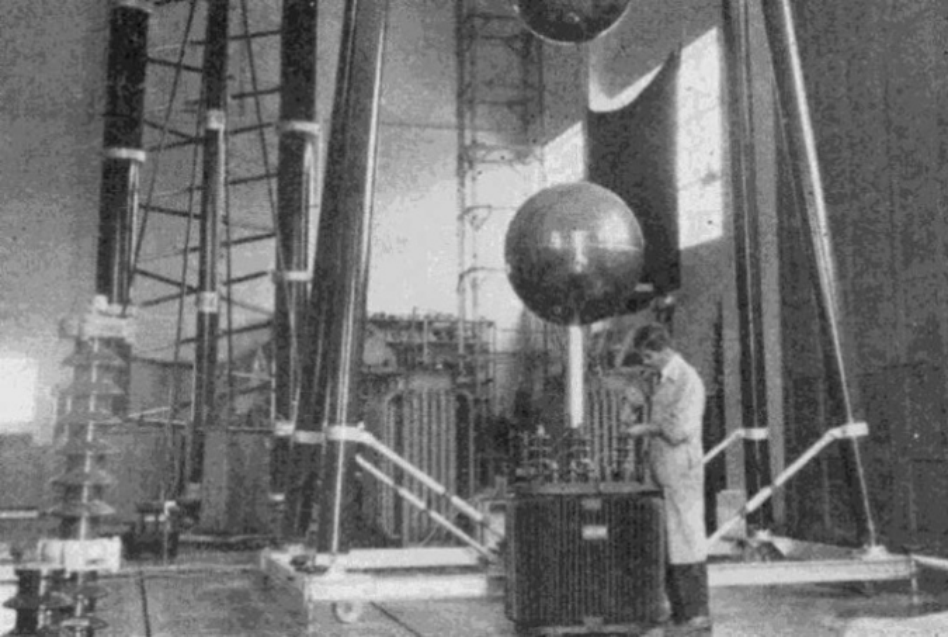
\includegraphics[width=\columnwidth]{./pictures/historia_DIE.png}
\caption{Laboratorio del Instituto de Investigaciones y Ensayos Eléctricos.}
\label{hist_die}
\end{figure}

El IIEE fue constituido por el Laboratorio de Alta Tensión, el Laboratorio de Electrotecnia y
el Laboratorio de Electrónica y Telecomunicaciones. Luego de tres años, se incluyó el Laboratorio
de Computadores y Control Automático.

En el período 1968 – 1969 en la Facultad se llevaron a cabo cambios y creaciones de gran
importancia, aprovechando un período que, en parte, fue motivado por la influencia global que
tuvieron los eventos estudiantiles ocurridos en Francia durante ese período. En este período se
realizó en la Facultad una substancial reforma docente. Se revisaron los planes de estudio y los
programas de los cursos y se instauró un sistema semestral, en vez del sistema anual.

En 1969, con apoyo de la Organización de Estados Americanos OEA, se creó el primer
programa de Magíster en Ingeniería Eléctrica. El Departamento había sido declarado Centro de
Excelencia por la OEA. Por una parte, esto permitió contratar profesores de Estados Unidos y
Europa; por otra, varios alumnos extranjeros pudieron seguir el programa y obtener el grado
de magíster. En el año 1985, en concordancia con una evolución y expansión de las áreas del
departamento, se crea el actual programa de Magíster en Ciencias de la Ingeniería, Mención
Eléctrica.

En 2005, se creó el programa de Doctorado en Ingeniería Eléctrica del que se han graduado
32 doctores y que actualmente cuenta con 53 alumnos.

El año 2006 se inició un profundo proceso de Reforma Curricular de las distintas
especialidades de las carreras de Ingeniería Civil, implementándose a partir de los ingresados el año
2007 al Plan Común de Ingeniería y a partir de 2009 para la especialidad de Ingeniería Eléctrica.
El Decreto Universitario N$^\circ$~0025028 [\ref{dec25028}] de 10 de octubre de 2008 de la Universidad de Chile,
estableció el nuevo plan de estudios para la licenciatura en Ciencias de la Ingeniería, mención
Eléctrica, y para la carrera de Ingeniería Civil Eléctrica. Este mismo decreto establece el cambio
de nombre de la carrera de Ingeniería Civil Electricista, pasando a llamarse Ingeniería Civil
Eléctrica.

Para la Reforma Curricular del 2007-2009 se realizó la elaboración de programas de cursos de
la carrera, proponiendo nuevas metodologías docentes, unificando criterios de evaluación y malla
de requisitos, e incluyendo en estos nuevos programas de curso las competencias profesionales y
genéricas de la carrera. Se implementaron estrategias metodológicas de aprendizaje y enseñanza
en varios cursos de la carrera.

El decreto Universitario N$^\circ$~0027663 [\ref{dec27663}] de 5 de noviembre de 2008 incorporó la variable de
género en grados académicos y títulos profesionales de la Universidad de Chile.

En el año 2007 la carrera Ingeniería Civil Electricista se sometió por primera vez a un proceso
de acreditación ante la Comisión Nacional de Acreditación (CNAP), donde fue acreditada por el
máximo de 7 años. En el último proceso del año 2015, la carrera de Ingeniería Civil Eléctrica fue
acreditada nuevamente por el máximo de 7 años, que culminan el 23 de enero de 2022. Por su parte,
el Programa de Magíster en Ciencias de la Ingeniería Mención Eléctrica, se encuentra acreditado
por un período de 6 años que finalizan el 21 de abril de 2016. A su vez el programa de Doctorado
se encuentra acreditado por un período de 8 años hasta el 09 de noviembre de 2019.

Entre los logros históricos del DIE se encuentran:
\begin{itemize}
\item En 1957 contribuyó con la planificación de la electrificación del país.
\item En 1962 instaló, operó y administró el primer computador digital en la Universidad de Chile.
\item En 1969, con apoyo de la OEA, creó el primer programa de Magíster en Ingeniería Eléctrica.
\item En 1973 diseñó y construyó el primer transistor bipolar en Chile.
\item En 1974 organizó el primer Congreso Chileno en Ingeniería Eléctrica y creó la Asociación Chilena de Control Automático (ACCA).
\item En 1976 diseñó y construyó el primer circuito integrado en el país.
\item En el año 1985 creó el actual programa de Magíster en Ciencias de la Ingeniería, Mención Eléctrica.
\item En 2005 creó el actual programa de Doctorado en Ingeniería Eléctrica.
\item En 2007 diseñó y construyó el primer automóvil de energía solar en Chile.
\item En 2007 DIE firma acuerdo con Associated Universities Inc. (AUI) que opera y administra el Atacama Large Millimeter Array (ALMA).
\item En 2009 se creó el programa de Magíster en Ingeniería de Redes de Comunicaciones. 
\item En marzo de 2009 se crea el Centro Avanzado de Tecnología para la Minería (AMTC).
\item En junio de 2009 nace el Centro de Energía (CE).
\item En 2010 diseñó, construyó y puso en marcha la primera micro-red inteligente con Energías Renovables No Convencionales (ERNC).
\item En 2014 se crea ECODIE, unidad de Educación Continua del DIE.
\item En 2015 se crea la primera plataforma solar del país instalada en Atacama.
\item En 2017 se lanza el primer satélite chileno al espacio.
\item En 2017 programa de doble doctorado en Ingeniería Eléctrica U. de Chile y U. de Nottingham tiene su primer graduado.

\end{itemize}

\subsection{Contexto del DIE}

\subsubsection{Infraestructura del DIE}

El DIE cuenta con un edificio de 8 pisos de propiedad institucional (6 sobre suelo y 2
subterráneos), donde se encuentran 6 salas de clases, oficinas administrativas y de los académicos
del departamento, salas de reuniones, laboratorios docentes y de investigación, un taller metalmecánico y una moderna sala de computadores.

\begin{figure}[ht!]
\centering
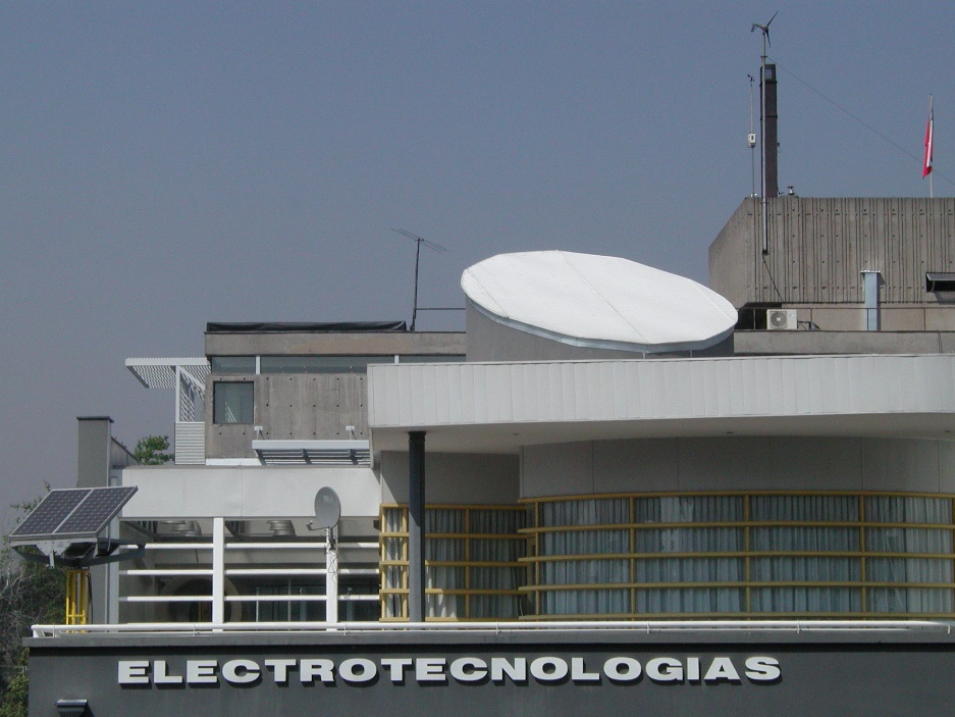
\includegraphics[width=\columnwidth]{./pictures/electrotecnologias.png}
\caption{Edificio de Electrotecnologías.}
\label{edif_ET}
\end{figure}

El DIE posee una infraestructura para labores docentes y experimentales de excelencia, lo
que permite un adecuado desarrollo de sus actividades de formación e investigación. Cuenta
hoy día con la infraestructura más importante del país en la especialidad con alrededor de
7.000 m$^2$. Esto incluye el edificio de Electrotecnologías, remodelado el año 2003, donde
se dispone de 8 laboratorios docentes de pregrado de ICE. Además, existen 15 laboratorios
de investigación en el departamento. Académicos y estudiantes trabajan conjuntamente en la
resolución de problemas complejos utilizando tecnologías de punta. Estas actividades cuentan
con financiamiento gubernamental de CONICYT, CORFO y MILENIO, así como también de
organizaciones internacionales y de aportes empresariales. El funcionamiento de los laboratorios
de investigación, así como la compra de equipamiento menor y mayor, se financia adecuadamente
con los proyectos de investigación dirigidos por los académicos del DIE.

La Tabla \ref{labs_die} muestra que a través de fondos concursables e inversiones de Facultad y DIE
se han creado 6 laboratorios nuevos a partir del año 2008, con una inversión total de
\$1.692.500.000. Cabe destacar que el Laboratorio de Ondas Milimétricas y Sub-milimétricas
es parte de una colaboración entre el DIE y el DAS, y se encuentra físicamente en este último.
Además el laboratorio es liderado por el Dr. Patricio Mena (académico del DIE) en conjunto con el
Dr. Leonardo Bronfman (académico del DAS).

\begin{table}[t!]
\centering
\caption{Inversión en Laboratorios Nuevos DIE desde el año 2007.}
\label{labs_die}
\begin{tabular}{lll}
\hline
& Año & Fuentes  \\ \hline \hline %& Inversión {[}CLP{]}
Laboratorio de Fotónica & 2008 & FCFM; CONICYT \\ %& 178.000.000 \\
\begin{tabular}[c]{@{}l@{}}Laboratorio de Ondas \\ Milimétricas y \\ Submilimétricas\end{tabular} & 2008 & \begin{tabular}[c]{@{}l@{}}Centro Basal de \\ Astrofísica y \\ Tecnologías Afines; \\ Fondos Concursables\end{tabular} \\ % & 870.000.000 \\
\begin{tabular}[c]{@{}l@{}}Laboratorio de \\ Exploración Espacial \\ y Planetaria (LEEP)\end{tabular} & 2010 & SUCHAI \\ % & 4.000.000 \\
\begin{tabular}[c]{@{}l@{}}Laboratorio de \\ Electrónica de Potencia, \\ Accionamientos y \\ Generación Distribuida\end{tabular} & 2011 & \begin{tabular}[c]{@{}l@{}}FCFM; DIE; \\ FONDECYT; \\ FONDEQUIP\end{tabular} \\ % & 600.000.000 \\
Optical \& Wireless Laboratory & 2011 & \begin{tabular}[c]{@{}l@{}}FCFM; DIE; \\ VID; FONDECYT\end{tabular} \\ % & 19.000.000 \\
Laboratorio de Acumuladores & 2012 & FCFM; DIE; CIL \\ \hline % & 21.500.000 \\ \hline
% & & \multicolumn{1}{r}{\textbf{TOTAL}} \\ \hline %& <.#laboratorioDIE.total_inversion#.> \\ \hline
\end{tabular}
\end{table}

\subsubsection{Planta Docente del DIE}

%La Tabla \ref{horas_jornada} presenta el número de académicos de jornada completa y parcial para los últimos <.#total_de_anos#.>
%años. Al <#planta_docente_ano(3)#> el cuerpo docente de Ingeniería Civil Eléctrica se compuso de <.#docentes_JC_DIE(3)#.> de académicos de
%jornada completa con doctorado, y <.#docentes_hora_DIE(3)#.> académicos de jornada parcial. Dentro del cuerpo académico,
%además de doctores en ingeniería eléctrica, se encuentran expertos de las industrias involucradas
%en la carrera como lo son: telecomunicaciones, energía, automática, etc.

%\begin{table}[ht]
%\centering
%\caption{Número y horas docentes de la carrera, según jornada de contrato.}
%\label{horas_jornada}
%\begin{tabular}{llll}
%\hline
%Año                                 		& <#planta_docente_ano(1)#> & <#planta_docente_ano(2)#> & <#planta_docente_ano(3)#> 
%N$^\circ$~docentes jornada completa        	& <.#docentes_JC_DIE(1)#.>  & <.#docentes_JC_DIE(2)#.>  & <.#docentes_JC_DIE(3)#.>  \\
%Horas docentes\footnote{Horas efectivas de clases a la semana} jornada completa    		& <.#horas_docentes_JC_DIE(1)#.>  & <.#horas_docentes_JC_DIE(2)#.>  & <.#horas_docentes_JC_DIE(3)#.>  \\
%											&   &   &   \\
%N$^\circ$~docentes contratados por hora    	& <.#docentes_hora_DIE(1)#.>  & <.#docentes_hora_DIE(2)#.>  & <.#docentes_hora_DIE(3)#.>  \\
%Horas docentes contratados por hora 		& <.#horas_docentes_hora_DIE(1)#.>  & <.#horas_docentes_hora_DIE(2)#.>  & <.#horas_docentes_hora_DIE(3)#.>  \\
%											&   &   &   \\ \hline
%Total docentes                      		& <.#docentes_DIE_total(1)#.>  & <.#docentes_DIE_total(2)#.>  & <.#docentes_DIE_total(3)#.>  \\
%Total horas                         		& <.#horas_docentes_DIE_total(1)#.>  & <.#horas_docentes_DIE_total(2)#.>  & <.#horas_docentes_DIE_total(3)#.>  \\ \hline
%\end{tabular}
%\end{table}

En la Tabla \ref{docentes_grados} pueden observarse las estadísticas de los académicos según grado académico
en el DIE. Todos los profesores de jornada completa del DIE poseen el grado de doctor, mientras
que entre los profesores de jornada parcial hay 3 doctores y 6 magísteres.

\begin{table}[ht]
\centering
\caption{Número de docentes según grado académico.}
\label{docentes_grados}
\begin{tabular}{llll}
\hline
Año                        			& 2017 \\ \hline \hline %2011 & 2012 & 2013 \\ \hline \hline
N$^\circ$~Doctores (PhD)        	& 28 \\ %21  & 22  & 24  \\
N$^\circ$~Magíster              	& 6 \\ %6  & 6  & 6  \\
N$^\circ$~Licenciados o titulados 	& 15 \\ %37  & 34  & 32  \\ \hline
\textbf{Total}             			& 49 \\ %64  & 62  & 62  \\ \hline
\end{tabular}
\end{table}

\subsubsection{Perfil de los estudiantes del DIE}

El DIE recibe a sus alumnos provenientes del Plan Común de la FCFM, cuyo perfil se
encuentra detallado en la Sección \ref{prefil_fcfm} ``Perfil de los estudiantes de la FCFM''.

Una de las principales fortalezas de los alumnos que ingresan a estudiar la carrera de Ingeniería
Civil Eléctrica, es su alto nivel académico. La Figura \ref{puntajes_psu_ice} muestra los promedios ponderados PSU
para estudiantes del Plan Común y de Ingeniería Civil Eléctrica. Se observa que los puntajes
obtenidos por los estudiantes de ICE, se encuentran por encima del promedio del Plan Común de
la Facultad.

\begin{figure}[ht]
\centering
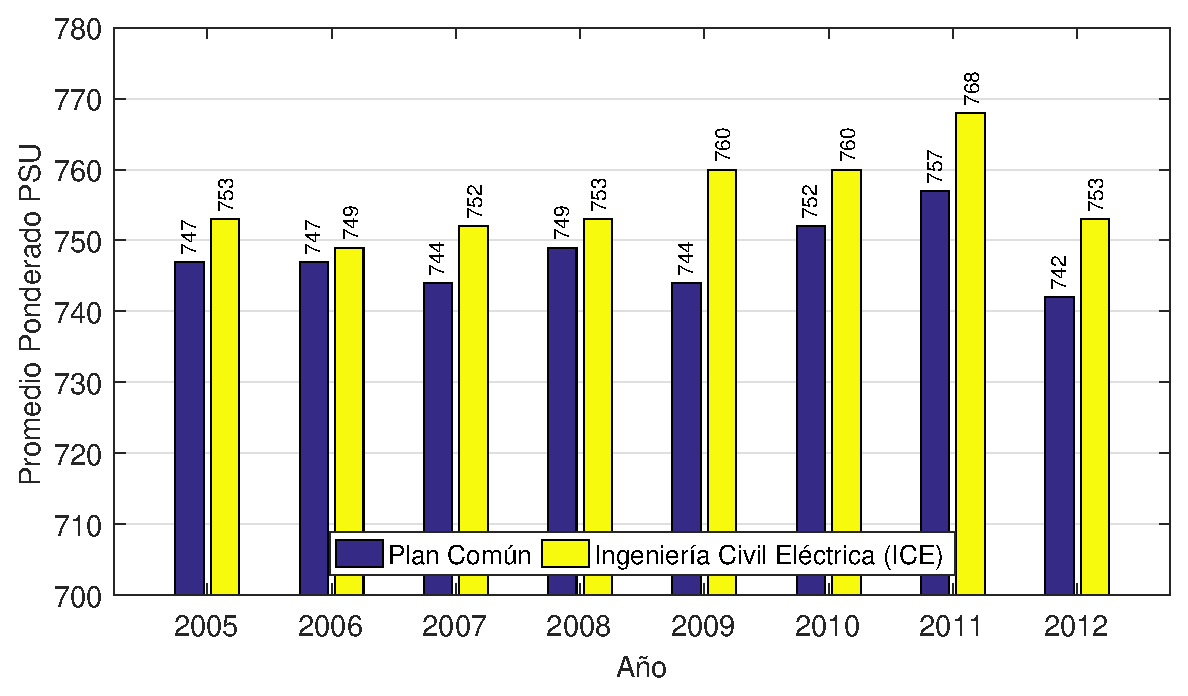
\includegraphics[width=\columnwidth]{./pictures/puntajes_psu_ice.eps}
\caption{Puntajes promedio PSU para estudiantes del Plan Común y del ICE.}
\label{puntajes_psu_ice}
\end{figure}

%En cuanto a género, se ve una disminución en el porcentaje de mujeres que ingresa a la carrera,
%con respecto al Plan Común. En este último, las mujeres representan cerca del 20\% del total de los
%estudiantes, mientras que en ICE es apenas cercano al 7\%. La Tabla \ref{matricula_genero} muestra el número de
%estudiantes de ICE por género entre los años 2011 y 2013.

%\begin{table}[ht]
%\centering
%\caption{Matrícula por género a ICE.}
%\label{matricula_genero}
%\begin{tabular}{llll}
%\hline
%Año                     & <#anos_estadisticas_genero_DIE(1)#> & <#anos_estadisticas_genero_DIE(2)#> & <#anos_estadisticas_genero_DIE(3)#> \\ %\hline \hline
%Matrícula total hombres & <.#matricula_hombres_ice(1)#.>  & <.#matricula_hombres_ice(2)#.>  & <.#matricula_hombres_ice(3)#.>  \\
%Matrícula total mujeres & <.#matricula_mujeres_ice(1)#.>  & <.#matricula_mujeres_ice(2)#.>  & <.#matricula_mujeres_ice(3)#.>  \\ \hline
%\textbf{Total}          & <.#matricula_total_ice(1)#.>  & <.#matricula_total_ice(2)#.>  & <.#matricula_total_ice(3)#.>  \\ \hline
%\end{tabular}
%\end{table}

\subsection{Descripción de la unidad académica}

El esquema docente en la FCFM, basado en un Plan Común inicial, está diseñado para lograr
que nuestros estudiantes alcancen un muy buen nivel base en Matemáticas y Física, permitiendo
un máximo aprovechamiento de las temáticas tratadas con posterioridad. La gran fortaleza del
Plan Común consiste en entregar herramientas para una adecuada adaptación de los educandos
a los veloces cambios en el conocimiento. Por otro lado, los estudiantes deciden finalmente
su especialidad, de manera informada y fundada, al cabo de 4 semestres de permanencia en la
Facultad. La FCFM ofrece 10 diferentes carreras profesionales y 3 licenciaturas, a las que acceden
nuestros estudiantes posteriormente a su aprobación del Plan Común, entre ellas Ingeniería Civil
Eléctrica (ICE). El año 2007 comenzó la más profunda reforma curricular de la carrera de Ingeniería
Civil Eléctrica de los últimos 40 años. Para esto se definió un nuevo perfil de egreso basado en
competencias que se desarrollan a lo largo de la carrera y que fueron agrupadas en competencias
profesionales (técnicas) y competencias genéricas, las cuales se encuentran publicadas en la página
web del DIE\footnote{\url{http://www.die.cl}}. El perfil de egreso antiguo se basaba en los contenidos de las materias para declarar
las habilidades requeridas por el profesional que egresaba. Para el nuevo plan de estudio, la
definición de perfil de egreso se centra en las habilidades para aprender y utilizar los contenidos,
lo cual se define como las competencias. En particular se utilizó la metodología CDIO. Las
competencias del nuevo perfil se diseñaron tomando en cuenta los adelantos en la disciplina, los
propósitos y misión de la institución, y se validó con empresarios externos.

\section{Magíster en Ingeniería de Redes de Comunicaciones}

\subsection{Breve historia del Programa}

Desde sus orígenes, la Universidad de Chile ha hecho contribuciones de primera importancia a
la formación del pensamiento crítico y al desarrollo de la nación. En docencia de postgrado
se revela una tradición que comienza en el año 1947 con la creación del primer doctorado en
Filosofía de la Facultad de Filosofía y Educación, y que se extiende hasta hoy con el sistema
de postgrado y postítulo más grande y complejo del país, compuesto por 36 programas de
doctorado, 118 programas de magíster, 75 programas de título profesional especialista y 27 cursos
de especialización de postítulo. El Departamento de Ingeniería Eléctrica es un fiel exponente de
esto, en donde destaca hoy en día el Doctorado en el área tecnológica con más años de acreditación
en la Universidad de Chile (8 años)5. Una fortaleza importante radica en la reglamentación existente
que cubre políticas institucionales de desarrollo del postgrado, estándares, calidad exigida a los
profesores y estudiantes, exigencias de investigación.

% En el año 1985, en concordancia con una evolución y expansión de las áreas del departamento,
% se crea el actual programa de Magíster en Ciencias de la Ingeniería, Mención Eléctrica [A.4]. No
% obstante, nuestro departamento tiene una larga historia en programas de Magíster, donde destaca
% el Magíster de Ingeniería Eléctrica que data de 1969. El Programa ha sido acreditado dos veces
% por la CONAP (actual CNA). El primer proceso fue el 2005 donde fue acreditado por un periodo
% de 4 años [A.5], siendo re-acreditado el 2010 por 6 años [A.6]. Esto lo posiciona dentro de los
% programas con mayor años de acreditación dentro de su área en la Universidad de Chile. El actual
% proceso corresponde a una segunda re-acreditación que apunta a un tramo de evaluación mayor, en
% relación a las mejoras realizadas desde la última acreditación.

En el 2010, el programa de Magíster en Ingeniería de Redes de Comunicaciones nace para atender la urgente necesidad que durante la primera década de nuestro siglo aquejaba a la industria de las telecomunicaciones en Chile, a saber, la falta de profesionales con especialización en tecnologías IP que tuvieran una formación neutra y un conocimiento agnóstico a lo que ofrecían los proveedores de tecnología.

Fue en una continuidad natural del postítulo en Internetworking, también de nuestra universidad, que formó cerca de 200 profesionales realizaron el desarrollo de sus habilidades prácticas con los laboratorios del Departamento de Ingeniería Electrica de la Facultad de Ciencias Físicas y Matemáticas. La proyección de los ex-alumnos de este postítulo requerían un complemento que les permitiera ampliar sus conocimientos de Internetworking, fundamentalmente en Routing, Switching IP y Telefonía tanto circuital como de paquetes IP, y poder ejercer su profesión en los operadores de telecomunicaciones que por esa fecha se perfilaban como convergentes tanto en tecnologías (circuitos y paquetes) como en servicios (telefonía y datos).

Es en ese contexto en que el programa se dicta por primera vez en el año 2010, con el incondicional impulso del entonces director del DIE, el profesor Nicolás Beltrán Maturana. Los tres primeros graduados del programa, dictado en un formato de magíster profesional al estilo de MBA de las telecomunicaciones con elementos de Informática, incorporando las tecnologías inalámbricas de punta en esos días, hacen sus recuerdos: “El ingreso y estadía en el programa MIRC se debe en gran parte al director del departamento de ese momento, el profesor Sr. Nicolás Beltrán, quién siempre me ayudo en el aspecto académico y administrativo“, dice Alberto Castro. Por su parte, Jorge Sandoval, al igual que Castro, un profesional de primera línea en nuestra industria, comenta: “La formación que recibí en el MIRC me abrió muchas puertas y el mercado reconoció mi condición de magíster aplicado a las necesidades de nuestra industria y con gran potencial de actualización, especialmente en las tecnologías y los servicios inalámbricos“. El tercero de la primera generación de graduados, Minflen Torres, también destacó por su orientación a las tecnologías inalámbricas dada su sólida formación en el MIRC, desarrollando una excelente carreta profesional en Entel, operador en el que trabaja hasta la actualidad.
La llegada del profesor Claudio Estévez en el año 2013 como coordinador al programa, le dio impulso a un programa diversificado que incluyó tópicos de Cloud Computing, IoT, Big Data Analytics, Evolución de 4G a 5G, Smart Cities, Regulación y Economía en las Telecomunicaciones, entre otros  temas de punta tanto tecnológica como de negocios, imprimiendo un enfoque fuertemente orientado a las necesidades de la industria de telecomunicaciones de estos días en que los operadores convergentes son una realidad que coexiste con los operadores Over The Top y los operadores virtuales.

El cuerpo académico, tanto en el claustro como en el equipo extendido de profesionales que trabajan en la industria, ha evolucionado desde Beltrán hasta Estévez para mantener actualizada la oferta de materias, siempre considerando las necesidades del país, la formación y en el perfeccionamiento de profesionales que destaquen por su visión sistémica y sus sólidos conocimientos tanto teóricos como prácticos.


\subsection{Proyecto académico de la unidad}

Este Programa otorga una formación con énfasis en la ingeniería avanzada y tecnologías
modernas de las redes de comunicación, que permitan a los graduados contribuir al desarrollo de sus países y satisfacer las
necesidades de la sociedad. Ofrece una formación profunda para
aquellas personas que desean orientar sus estudios hacia actividades de innovación tecnológica y docencia superior.

Lo(a)s ingeniero(a)s que ingresan pueden profundizar sus estudios en áreas como Smart Cities, Internet de las Cosas, Cloud Computing, 
técnicas de modulación, protocols de acceso, protocolos de transporte, enrutamiento, comunicación vehicular, eficiencia energética
en sistemas de comunicación, modelamiento de redes, calidad de servicio y experiencia en redes móviles, comunicación inalámbrica avanzada, 
seguridad de redes y muchos otros tópicos más. El cuerpo académico cubre una amplia diversidad de tópicos, esto para poder cumplir 
los objetivos del programa.


%----------------------------------------------------------------------------------------
%	CHAPTER 2
%----------------------------------------------------------------------------------------

\chapterimage{proceso_formativo.jpg}
\chapter{Criterios de Evaluación}
Toda la información del presente capítulo ha sido obtenida de las diferentes fuentes que tiene la
Universidad de Chile tanto físicas como digitales que se especifican a lo largo del documento.
Además, se utilizó la información obtenida de una encuesta realizada a estudiantes, graduados
y académicos del Programas para enriquecer el informe y validar la información entregada en
diversos aspectos relativos al Programa. En varias secciones de este Capítulo nos referiremos a los
resultados de la encuesta pero sus detalles son presentados en la Sección \ref{encuestas} del presente informe.

\section{Definición Conceptual}

El Magíster en Ingeniería de Redes de Comunicaciones (en adelante mencionado
indistintamente por su nombre completo o como ``el Programa''), se encuentra en concordancia
con el Reglamento General de Estudios Conducentes a los Grados de Magíster y Doctor, Decreto
Universitario N$^\circ$~0028011 de octubre del año 2010 de la Universidad de Chile [\ref{reg_mag_doc}]. Este
Reglamento en su artículo 23 establece que:

\textit{``Un Programa conducente al grado de Magíster debe entregar conocimientos y competencias que
habiliten a los graduados para abordar asuntos complejos en forma sistemática y creativa. Estos
deben demostrar originalidad en la aplicación del conocimiento a través del planteamiento y la
resolución de problemas. Los Programas podrán orientarse al desarrollo de capacidades para:
La investigación, la innovación tecnológica, la creación artística o el desempeño profesional
superior.''}

En este contexto, el Programa se ha definido con el objetivo de ofrecer una formación profunda
en las redes de comunicaciones. Está diseñado para aquellas personas que deseen orientar
sus estudios hacia actividades principalmente de desarrollo y docencia superior. Es así como el
Programa corresponde a un Magíster de carácter profesional, presencial a tiempo completo y de
jornada vespertina. Esto es plenamente concordante con lo definido por la CNA para los Programas
de Magíster. 

% El Programa posee una articulación natural con la Carrera de Ingeniería Civil
%Eléctrica (ICE) de la Facultad de Ciencias Físicas y Matemáticas de la Universidad de Chile, del
%cual proviene un 71\% de sus estudiantes (ver Sección \ref{prog_eval}). Esta articulación permite que los
%estudiantes de ICE que postulen al grado de Magíster, ya sea simultáneamente o después de obtener
%su título profesional de Ingeniería, puedan convalidar UDs obtenidas por cursos de nivel 6000
%(electivos de la carrera de ICE) así como cursos electivos de nivel 7000 (electivos de postgrado).
%Se destaca el caso de los estudiantes que optan por doble titulación en el momento de realizar su
%trabajo de titulación en paralelo con la Tesis de Magíster, permitiendo en algunos casos el doble
%grado de Ingeniero y Magíster en 6 años y medio. Todo esto en concordancia con el Reglamento
%General de Magíster y Doctorado de la Universidad de Chile [\ref{reg_mag_doc}] y con el reglamento Interno
%de Magíster [A.8]. Asimismo, el carácter académico del Magíster permite la articulación con el
%Programa de Doctorado en Ingeniería Eléctrica en forma natural. Dicha articulación se desarrolla
%a nivel académico con estudiantes de Magíster que continúan en el Doctorado. Desde la Dirección
%del Departamento de Ingeniería Eléctrica los esfuerzos se han orientado a reforzar la sinergia
%del postgrado en el área eléctrica. Por lo anterior, desde el año 2012, los comités académicos
%del Magíster y el Doctorado se han fusionado para sesionar actualmente como un único Comité
%Académico de Postgrado del Departamento de Ingeniería Eléctrica.

\section{Contexto Institucional}
\label{contexto_institucional}

\subsection{Estructura Organizacional Institucional}

\subsubsection{Vicerrectoría de Asuntos Académicos}

Dentro de las vicerrectorías mencionadas en la Sección \ref{historia}, la Vicerrectoría de Asuntos
Académicos (VAA) tiene relación directa con la normalización de los planes de estudios de pre y
postgrado de la Universidad de Chile, la atención integral de los estudiantes, la selección y admisión
de alumnos, y las actividades de autoevaluación institucional, entre otras.

Su ámbito de trabajo cubre todo el espectro de la vida académica y de formación integral de
los estudiantes de pregrado y postgrado, incluyendo la selección y admisión de alumnos a través
de la PSU para todo el sistema universitario. Con una perspectiva de aseguramiento de calidad,
y en colaboración con las unidades académicas, define políticas para el desarrollo, creación y
modernización de los Programas de estudios de Pre y Postgrado, así como en el otorgamiento
de servicios académicos de bienestar y de recreación a los estudiantes atendiendo a su equidad.

Además, la Vicerrectoría presta apoyo técnico a las Facultades, Escuelas e Institutos
principalmente en su gestión curricular y procesos de acreditación, y mantiene información
actualizada de la calidad académica de la Universidad.

Según el articulo 16 del Reglamento General de Estudios Conducente a los Grados de Magíster
y Doctor (Decreto Universitario N$^o$0028011 de 5 de octubre de 2010) [\ref{reg_mag_doc}], la VAA velará
por la calidad de los Programas de postgrado, sometiéndolos a acreditación interna y externa,
estableciendo los organismos y procedimientos para cada caso. En particular según el articulo 17
del mismo reglamento, para efecto de la acreditación interna la VAA deberá considerar, al menos:

\begin{itemize}
\item Idoneidad y tamaño del claustro de profesores del Programa;
\item Líneas de investigación que sustenten el Programa;
\item Efectividad del proceso de enseñanza aprendizaje;
\item Coherencia entre los objetivos del Programa, el perfil de graduación y sus resultados;
\item Infraestructura y disponibilidad de servicios y recursos educacionales, y
\item Mecanismos implementados para el aseguramiento de la calidad.
\end{itemize}

En lo referente a Postgrado, la Vicerrectoría de Asuntos Académicos posee un Departamento
de Postgrado y Postítulos (DPP). Este tiene como finalidad cautelar y estimular el desarrollo de
los estudios conducentes a los grados de Magíster y Doctorado, y de cursos de especialización
profesional en todas las unidades académicas del plantel. De igual forma, articula los recursos
humanos y materiales en relación a la creación de nuevos grados académicos y cautela la idoneidad
y calidad de los Programas que ofrece la Casa de Estudios.

En este sentido el DPP trabaja en estrecha relación con la Escuela de Postgrado de la FCFM,
así como con las otras unidades del área académica de la Vicerrectoría de Asuntos Académicos,
con la Vicerrectoría de Investigación y Desarrollo, y la Dirección de Relaciones Internacionales
(dependiente de Rectoría) de la Universidad de Chile.

En cumplimiento de su misión, brinda asistencia en la formulación, revisión y actualización
de Programas de Magíster y Doctorado y de especialización profesional, y homogeneiza normas y
reglamentos atingentes a la materia. Por otra parte, administra la asignación de recursos de becas
para estudiantes meritorios y desarrollo de tesis.
Asimismo promueve el ingreso de alumnos extranjeros a los Programas de postgrado y de
especialización.

\subsubsection{Acreditación Institucional 2011 - 2018}

%El 21 de diciembre de 2011 la Universidad de Chile recibió oficialmente la acreditación
%institucional por parte de la Comisión Nacional de Acreditación - CNA, por el periodo máximo
%de tiempo de siete años -hasta el 21 de diciembre de 2018- tras registrar positivas evaluaciones
%en todas las áreas de evaluación, tanto aquellas obligatorias -gestión institucional y docencia de
%pregrado- como en aquellas electivas -investigación, docencia de posgrado y vinculación con el
%medio-. Esto fue expuesto en el Acuerdo N$^o$161 de la Comisión Nacional de Acreditación CNA
%[A.9].

%Se destaca en el área de docencia de Postgrado (extraído del acuerdo N$^o$ 161 de la CNA):

%\begin{itemize}
%\item Se registra un claro liderazgo Institucional en el área de Postgrado y una numerosa oferta
%de Programas de calidad, cuya provisión se encuentra debidamente normada mediante
%la existencia de políticas y mecanismos que regulan su oferta. En especial se destacan
%los mecanismos de aseguramiento de calidad de los Programas de doctorados, los cuales
%presentan una importante contribución social a nivel nacional.
%\item La universidad presenta infraestructura física, biblioteca y servicios estudiantiles adecuados
%para la oferta de Programas de postgrado. Asimismo, se constata la existencia de mecanismos
%de aseguramiento de la calidad de la docencia, lo cual permite contar con académicos de
%destacado nivel.
%\item Se constata la existencia de una rica actividad académica, la cual es alimentada por visitas
%de profesores, intercambios estudiantiles, realización de tesis en co-tutela, pasantías y
%convivencia con investigadores de post doctorado. Igualmente se evidencia un claro traspaso
%de las actividades investigativas a la docencia de postgrado. La generación de publicaciones
%a nivel internacional y la participación de los estudiantes en dichas actividades son un claro
%ejemplo de aquello.
%\end{itemize}

%Se destaca en el área de Investigación (extraído del acuerdo N$^o$ 161 de la CNA):
%\begin{itemize}
%\item La Universidad de Chile presenta una tradición de cultivo de la investigación, siendo esta
%característica parte esencial de su ser universitario. Asimismo, presenta una alta calidad en
%su producción científica en relación a estándares nacionales e internacionales. De esta forma,
%la Universidad de Chile se sitúa en una posición de liderazgo a nivel nacional, cuenta con
%gran prestigio al respecto e impacta, con sus investigaciones, en el desarrollo del país.
%\item El quehacer investigativo de la Universidad permea todas las actividades institucionales.
%Se evidencia, especialmente, una importante vinculación con la docencia de postgrado; en
%particular lo que respecta a la interrelación con los Programas de doctorado y magísteres
%académicos.
%\end{itemize}

\subsubsection{Escuela de Postgrado}

El enlace de los Programas de Postgrado de la FCFM con la institucionalidad pertinente
(Departamento de Postítulo y Postgrado de la Universidad de Chile (DPP)) es a través de la Escuela
de Postgrado. Esta tiene como función organizar, administrar e impartir los estudios conducentes
a la obtención de grados académicos de Magíster y Doctor. Su máxima autoridad es su Director,
quien en conjunto con el Consejo de la Escuela de Postgrado pondrán en práctica las políticas de
desarrollo de la docencia de postgrado.

La Escuela de Postgrado asegura el funcionamiento operacional y académico de todos los
Programas de Postgrado de la FCFM. Además permite la sinergia de los mismos, la construcción
de criterios comunes, el crecimiento orgánico y el mejoramiento continuo.

\subsubsection{Normativas y Reglamentos}

El Programa se rige por los reglamentos de la Universidad de Chile nombrados a continuación y
que se adjuntan en los anexos respectivos.

El principal reglamento de postgrado de la Universidad de Chile es el Reglamento General
de Estudios Conducentes a los Grados de Magíster y Doctor [\ref{reg_mag_doc}]. Además posee un reglamento
general propio del Programa [\ref{reg_mirc}].

Dada la naturaleza de la Universidad de Chile, se exige tener un reglamento general con
las características definidas para éste, pero además se hace necesario y recomendable tener un
reglamento interno donde se estipulan, entre otros temas, los requisitos operativos y de gestión del
Programa. Actualmente se encuentra vigente el reglamento general del Programa del año 2006.
Además, está en fase de tramitación en los cuerpos colegiados de la Universidad de Chile, el nuevo
reglamento general del Programa, ambos en el Anexo correspondiente [\ref{reg_mirc}].

La estructura reglamentaria de la Universidad de Chile es clara en lo que respecta a los
Programas conducentes a los grados de magister y doctorado [\ref{reg_mag_doc}]. Esta reglamentación define
un marco sobre el cual se regulan los Programas tocando aspectos tales como la naturaleza del
Programa, sus objetivos y perfil de graduación, su creación, la administración, la conformación
del claustro, las responsabilidades del comité académico, las responsabilidades de la escuela
de postgrado, la acreditación y procesos de aseguramiento de calidad. Adicionalmente en este
Reglamento hay disposiciones específicas para los Programas de Magister que tocan aspectos
relativos a postulación y criterios de selección, plan de formación, proyecto de grado, actividad
de graduación, extensión mínima y máxima del Programa, homologación de UDs, criterios de
aprobación, entre otros. Complementando lo anterior el Programa consta de un Reglamento
General [\ref{reg_mirc}]. El primero establece aspectos reglamentarios
específicos que definen con mayor precisión el Programa, en el marco del Reglamento General de
la Universidad de Chile. Un ejemplo de ello es la definición concreta de los objetivos del Programa,
su plan de formación y su extensión en lo que respecta a número de UDs. Dichos reglamentos son
coherentes entre si y además deben ser revisados por el área jurídica de la Universidad así como
aprobados por los cuerpos colegiados respectivos. Finalmente, el Reglamento Interno se hace cargo
de las disposiciones operativas del Programa, como son, por ejemplo, estipular el Programa de
ayuda de viajes y los criterios arancelarios. Los Reglamentos Generales e Internos del Programa
se actualizan y revisan periódicamente por el Comité Académico del Programa, como se evidencia
en la renovación de los mismos en los últimos años.

\subsection{Sistema de Organización Interna}

\subsubsection{Organigrama del Departamento de Ingeniería Eléctrica}

El Departamento de Ingeniería Eléctrica de la Universidad de Chile tiene por su parte una
organización autónoma que vela por el buen funcionamiento tanto de la carrera de Ingeniería Civil
Eléctrica como de los Programas de postgrado (ver Fig. 2.1).

\begin{figure}[ht]
\centering
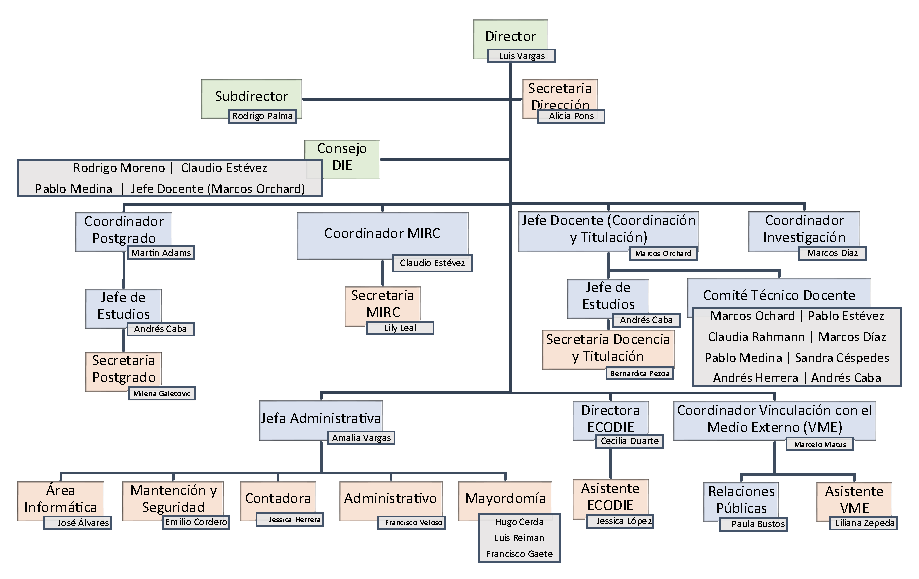
\includegraphics[width=\columnwidth]{./organigramas/die.eps}
\caption{Organigrama del Departamento de Ingeniería Eléctrica.}
\label{orga_die}
\end{figure}

Las funciones de Director de Departamento corresponderán a quien sea elegido por sus
académicos (jornada completa y parcial) conforme al Reglamento General de Elecciones y
Consultas [\ref{reg_elec_cons}], quien deberá ser un académico de las dos más altas jerarquías. Para cumplir
sus funciones deberá contar con una jornada contratada no inferior a 22 horas. Durará dos años en
sus funciones pudiendo ser reelegido por un periodo adicional.

El Reglamento General de Facultades [\ref{reg_gen_fac}] define las responsabilidades del Director de
Departamento como sigue:

\begin{enumerate}
\item Representar al Departamento ante el Consejo de Facultad y ante otras instancias.
\item Presidir el Consejo del Departamento.
\item Proponer al Decano la celebración de contratos de prestación de servicios y convenios de
honorarios.
\item Coordinar con los Directores de Escuela la realización de actividades de docencia que
correspondan al Departamento, para asegurar la calidad de la docencia impartida por los
miembros de su Departamento.
\item Presentar al Consejo del Departamento, para su aprobación, los planes anuales de desarrollo
académico de Departamento y su presupuesto, velando por su cumplimiento.
\item Entregar un informe fundado de las actividades de los académicos de su Departamento a la
Comisión de Calificación de su Facultad, con conocimiento por parte de cada interesado.
\item Presentar al Decano una cuenta anual sobre el funcionamiento académico y financiero del
Departamento para que éste la presente al Consejo de Facultad.
\item Proponer al Decano, con la aprobación del Consejo del Departamento, el nombre de la persona
que desempeñará la función de Subdirector, el cual colaborará en su gestión y lo subrogará en
caso de ausencia o impedimento. El subdirector deberá ser un académico de la categoría de
Profesor.
\item Determinar la creación de coordinaciones de apoyo a la Dirección cuando lo estime conveniente,
así como el nombre de las personas que desempeñarán esas funciones.
\item Las demás que le fija la reglamentación universitaria o que el Decano le delegue.
\end{enumerate}

El Consejo del Departamento se conforma por 6 académicos, 2 de ellos son parte de éste
por derecho propio (Director y Jefe Docente) y 4 son elegidos por el claustro académico. Los
consejeros de libre elección duran dos años en sus funciones, pudiendo ser reelegidos. Pueden
participar también, como invitados, representantes estudiantiles cuando las materias lo ameriten y
son elegidos de acuerdo a lo establecido por su organización estudiantil de Facultad.

Según el Reglamento General de Facultades [\ref{reg_gen_fac}] corresponde al Consejo de Departamento:

\begin{itemize}
\item Aprobar el plan anual de desarrollo académico y el presupuesto correspondiente.
\item Aprobar la proposición de un académico, hecha por el Director de Departamento, para que
aquél cumpla la función de Subdirector. Una vez aprobada, será propuesta al Decano.
\item Aprobar los planes de gestión de proyectos y servicios que someta a su consideración el
Director de Departamento.
\item Las demás que le asignen los reglamentos o que le encomiende el Director del Departamento.
\end{itemize}

El Subdirector cumple la función de subrogar al Director del Departamento en caso de
ausencia o impedimento de este.

La Oficina Administrativa controla, gestiona y ejecuta el presupuesto de la Unidad. La
Oficina Administrativa reporta a la Dirección Económica y Administrativa de la FCFM. Además
de los sueldos y remuneraciones, esta oficina gestiona la contratación de profesores part-time y
profesionales, los recursos de unidades de beca para el pago de auxiliares y ayudantes docentes,
adquisición de material bibliográfico, adquisición de equipamiento computacional y de laboratorio,
recursos de educación continua, y recursos de titulación y graduación. Además gestiona los
recursos humanos de la unidad, en particular mayordomos, estafeta, encargado de mantención
y electricidad, encargado de laboratorios docentes, encargado de taller mecánico. El Jefe
administrativo se selecciona en base a concurso público y la decisión para su selección es colegiada
y cuenta con la participación de las más altas autoridades administrativas de la Facultad. La actual
jefa administrativa del DIE es de profesión ingeniera comercial.

El Jefe Docente es nominado por el Director de Departamento y ratificado por el Decano.
Dentro de sus funciones está liderar el Comité Técnico Docente y participar en el Consejo de
Escuela. El Jefe Docente coordina todas las instancias relativas a la docencia de Ingeniería
Civil. Además está a cargo de la parte operativa, incluyendo atención de alumnos, solicitudes,
Programación de cursos, designación de profesores, etc. La implementación en el año 2007 de la
reforma curricular sumado a los procesos de acreditación y vertiginoso mercado laboral, exigen
una continua revisión de planes y Programas de estudio. Es por esto que como una forma de apoyar
la labor de los jefes y coordinadores docentes, cuyas funciones más urgentes tienen que ver con
la administración y gestión de la docencia, la Facultad de ciencias Físicas y Matemáticas propone
la conformación en cada departamento de Comités Técnicos Docentes (CTD), que con una mirada
integral de la carrera, apoyen el mejoramiento continuo de la docencia en el pregrado de la facultad,
contando con la asesoría de especialistas del Área de Desarrollo Docente (ADD) de la Escuela de
Ingeniería y Ciencias.

El Comité Técnico Docente (CTD) es elegido por el Jefe Docente y se conforma por al menos
2 académicos jornada completa (incluyendo al Jefe Docente), un académico de Jornada Parcial, y
al menos un estudiante de pregrado o postgrado.

El Jefe de Estudios cumple funciones administrativo académicas tanto en pregrado como en
postgrado. Su misión es apoyar en sus funciones al Jefe Docente y al coordinador de Postgrado.
El Coordinador de Innovación y Desarrollo potencia y lleva a cabo actividades relativas
a innovación y desarrollo tanto a nivel de departamento como con la interrelación con otros
departamentos de la Universidad de Chile.

El Coordinador de Educación Continua es el encargado de desarrollar y coordinar las
acciones de extensión del departamento. A su cargo está el EcoDie, unidad de educación continua
del departamento.

El Coordinador de Investigación enlaza y coordina las actividades de investigación de los
académicos del departamento.

Finalmente el Coordinador de Postgrado, así como el comité Académico de Postgrado, se
detallan a continuación en la sección de Gestión interna del Programa de Magíster. Tal como se
mencionó anteriormente, el Coordinador de Postgrado se apoya fuertemente en el Jefe de estudios
para la administración eficiente de los Programas.

\subsubsection{Gestión interna del Programa de Magíster Profesional}

El Programa de Magíster en Ingeniería de Redes de Comunicaciones, es administrado por la
Escuela de Postgrado de la Facultad de Ciencias Físicas y Matemáticas de la Universidad de Chile.
De acuerdo al Reglamento General de Estudios Conducentes a los Grados de Magíster y Doctor,
Decreto Universitario No0028011 de octubre del año 2010, de la Universidad de Chile [\ref{reg_mag_doc}], la
Facultad de Ciencias Físicas y Matemáticas de la Universidad de Chile debe poseer una Escuela
de Postgrado, la cual se encarga de la administración académica de los Programas de magíster
y doctorado. Para efectos de dicha administración, la Escuela de Postgrado es dirigida por un
Director, con la colaboración del Consejo de Escuela y el Comité Académico del Programa de Magíster en Ingeniería de Redes de Comunicaciones.

Dentro del DIE, el Programa cuenta con un Comité Académico, cuyos integrantes son
nombrados por el Director de Escuela, a proposición del claustro académico, y con el acuerdo
del Consejo de la Escuela de Postgrado de la FCFM. Este Comité Académico está conformado por
al menos tres profesores pertenecientes al claustro académico del Programa, quienes eligen a uno
de ellos como Coordinador. Los miembros del Comité Académico duran dos años en sus funciones,
pudiendo ser nominados por otros períodos.

En concordancia con el Reglamento General de Estudios Conducentes a los Grados de
Magíster y Doctor de la Universidad de Chile [\ref{reg_mag_doc}] en sus articulos 6 y 7, el Comité Académico se
responsabiliza por gestionar los aspectos académicos del Programa, velando por el cumplimiento
de sus objetivos, por el mejoramiento continuo del Programa y por la formación de sus estudiantes,
de acuerdo a estándares de calidad establecidos por la Universidad de Chile.

Las funciones del Comité Académico son:

\begin{itemize}
\item Seleccionar a los estudiantes que se incorporarán al Programa
\item Aprobar los planes de estudios de los postulantes
\item Nombrar a los respectivos profesores guías 
\item Aprobar al profesor guía de la tesis propuesto por cada estudiante
\item Proponer al Director de Escuela los integrantes de la comisión evaluadora de proyectos de
tesis, de la tesis y del examen de grado
\item Elaborar periódicamente un informe sobre el estado del Programa a su cargo, verificando el
cumplimiento de los indicadores de calidad definidos por la Facultad, y
\item Cautelar que la investigación que realicen los estudiantes considere las normas y
procedimientos propios de la disciplina.
\end{itemize}

Para estos efectos, el Comité Académico se sesiona periódicamente para analizar, debatir
y resolver sobre las distintas responsabilidades mencionadas anteriormente. En el último ano
el Comité ha sesionado a una tasa promedio de dos reuniones menusuales. Por otra parte, el
involucramiento del resto del claustro académico en términos de gestión y academia, radica en
buena medida en su rol como guias de tesis. No obstante, se realizan jornadas periódicas
a lo largo del año con el resto del claustro con el fin de formar un espacio para la discusión y el
debate en torno a las materias del Programa. En general el funcionamiento propende a la integración
total y continua del claustro en el desarrollo del Programa.

% En cuanto al fortalecimiento de la gestión diaria, atención de estudiantes, apoyo a profesores,
% manejo administrativo, entre otros, en los últimos años se ha impulsado el desarrollo del cuerpo de
% profesionales involucrados en la gestión del magíster y doctorado, así como la homologación de
% funciones de gestión interna en el departamento. En este contexto destacan los siguientes hitos:

% \begin{itemize}
% \item Fusión de los Comités Académicos de magíster y doctorado. Desde el año 2011 y en pos de
% una articulación cada vez más eficiente, se fusionaron los comités de Magíster y Doctorado
% del departamento.
% \item Contratación del Jefe de Estudios del Departamento de Ingeniería Eléctrica en Diciembre del
% 2014. Como se mencionó en la sección anterior, el Jefe de Estudios apoya las labores del
% Jefe Docente y del Coordinador de Postgrado. En virtud de lo anterior, este cargo potencia la
% articulación de la carrera de pregrado con el postgrado del Departamento.
% \item Contratación de una Secretaria de Postgrado en Diciembre del 2014. Este cargo fusiona las
% responsabilidades de la secretaria de magíster y secretaria de doctorado.
% \end{itemize}

% Cabe destacar de estas contrataciones el perfil requerido, donde se hizo especial hincapié en
% que dichos profesionales contaran con una amplia trayectoria en gestión universitaria. Se destaca
% además que la secretaria de Postgrado cuenta con estudios formales de idiomas.

\section{Características y Resultados del Programa}

\subsection{Carácter, objetivos y perfil de egreso}

\subsubsection{Definición del Programa}

El Magíster en Ingeniería de Redes de Comunicaciones, es un Programa de carácter profesional que, esencialmente, 
fue creado para formar a estudiantes en el área de redes de comunicaciones. 
Su plan de formación apunta a que los estudiantes se formen en tópicos
avanzados de telecomunicaciones y redes de comunicaciones. Esto les permite desarrollarse en la frontera del conocimiento
a través del ejercicio mismo del desarrollo que realizan bajo la cercana supervisión de los
profesores guías de tesis.

El Programa se encuentra perfectamente alineado con el perfil que establece la Universidad de
Chile. Este perfil se define explícitamente a través del Reglamento General de estudios conducentes
a los grados de Magíster y Doctor [\ref{reg_mag_doc}]. En su artículo 23, el reglamento estipula:

``Un Programa conducente al grado de Magister debe entregar conocimientos y competencias que
habiliten a los graduados para abordar asuntos complejos en forma sistemática y creativa. Estos
deben demostrar originalidad en la aplicación del conocimiento a través del planteamiento y la
resolución de problemas. Los Programas podrán orientarse al desarrollo de capacidades para: la
investigación, la innovación tecnológica, la creación artística o el desempeño profesional
superior.''

Por tanto, el Programa está dirigido a aquellas personas que deseen orientar sus estudios hacia
las actividades de innovación, desarrollo y docencia superior, en la disciplina de
Ingeniería Eléctrica con especialidad en Redes de Comunicaciones.

El Programa se rige por el reglamento General del Programa [\ref{reg_mirc}]. 
Dada las normas de la Universidad de Chile, se exige que los progamas tengan
un reglamento general que contenga las definiciones básicas del Programa. Adicionalmente es
necesario y recomendable contar con un reglamento interno donde se estipulan, entre otros temas,
los requisitos operativos y de gestión del Programa.

\subsubsection{Perfil de egreso}

\noindent\textbf{Objetivo general}

El Magister en Ingeniería de Redes de Comunicaciones (MIRC), de la Universidad de Chile, 
es un postgrado orientado a profesionales del área de tecnologías de comunicaciones que 
les permite profundizar y aplicar el conocimiento de redes de comunicaciones de última 
generación, gestión de proyectos de alta integración tecnológica, estudio de la economía 
que rodea a las telecomunicaciones, regulación chilena de las telecomunicaciones y la 
seguridad de las redes de comunicaciones. Este Programa equilibra aspectos teóricos, 
otorgando una sólida base conceptual en redes de comunicaciones, con factores imprescindibles 
en el ámbito profesional que habilitan al egresado a poner en práctica dicho conocimiento.

\noindent\textbf{Objetivos específicos:}

\begin{itemize}
\item Entregar una sólida base teórica sobre redes de comunicaciones y su aplicación en tecnologías 
inalámbricas, redes móviles y redes de banda ancha.
\item Formar profesionales que puedan reconocer tecnologías aplicadas de última generación para 
luego aplicarlas hábilmente en su medio laboral.
\item Entregar las herramientas para que puedan identificar y solucionar problemas de seguridad 
en redes complejas. 
\item Enseñar a gestionar calidad en redes móviles, formulando, diseñando y aplicando modelos de 
calidad de experiencia.
\item Habilitar el desarrollo de competencias profesionales necesarias para evaluar alternativas 
técnico-económicas, diseñar y gestionar proyectos tecnológicos y liderar iniciativas tecnológicas de punta.
\end{itemize}

\noindent\textbf{Descripción del Perfil de Egreso:}

Los graduados del Magíster en Ingeniería de Redes de Comunicaciones (MIRC) son profesionales habilitados para:

\begin{itemize}
\item Demostrar originalidad en la aplicación del conocimiento a través del planteamiento y la resolución de problemas en los siguientes ámbitos:
\begin{itemize}
\item Comunicación digital y analógica
\item Interconexión de redes
\item Redes multiservicios (incl. Cloud computing, IoT, Big Data, etc.)
\item Redes Inalámbricas (incl. móviles)
\item Desempeño de redes de comunicaciones
\item Gestión de proyectos de redes.
\end{itemize}
\item Adaptar, operar y gestionar redes de comunicaciones sobre la base de una capacidad analítica y sólidas bases en aspectos teóricos y aplicados. 
\item Conocer aspectos de regulación y economía de las telecomunicaciones.
\item Liderar, gestionar e implementar proyectos de redes de comunicaciones de última generación.
\end{itemize}

\noindent\textbf{Perfil de Egreso:}

Los graduados del Magíster en Ingeniería de Redes de Comunicaciones son profesionales capaces 
de aplicar el conocimiento a través del planteamiento y la resolución de problemas en el ámbito 
de las redes de comunicaciones. Los alumnos graduados poseen los conocimientos necesarios para 
la comprensión de nuevas tecnologías de comunicaciones a medida que surgen. También están preparados 
para adaptar, operar y gestionar redes de comunicaciones sobre la base de una capacidad analítica y 
sólidos fundamentos en aspectos teóricos y aplicados. Así mismo, están habilitados para liderar, 
gestionar e implementar proyectos de redes de última generación. Se espera que tengan conocimientos 
de regulación y economía orientado a las telecomunicaciones. Los egresados están preparados para 
realizar labores en el ámbito de las redes de comunicaciones y organismos regulatorios. 


\subsubsection{Revisión y difusión del perfil de egreso}

Los mecanismos de revisión y difusión del perfil de egreso, así como del carácter y los objetivos del
Programa, son continuos y diversos. Se posibilitan y ejecutan a través de las siguientes instancias
formales:

\begin{itemize}
\item Reuniones regulares del Comité Académico. 
\item Reuniones del subcomité encargado del Perfil de Egreso.
\item Revisión por parte del claustro y colaboradores del Programa.
\end{itemize}

Adicionalmente, la unidad de Gestión Curricular de la FCFM apoya los procesos de revisión
de los perfiles de egreso de Postgrado y Pregrado. Además, apoya el desarrollo curricular de las
carreras y Programas de Postgrado.

El perfil de egreso es también validado a través del contacto con alumnos y egresados,
utilizando encuestas. En particular, la última encuesta realizada producto del presente proceso
de auto evaluación (ver Sección \ref{caract_obj_perf_egr}) señala que:

\begin{itemize}
% \item En promedio, los egresados y alumnos activos del Programa, está muy
% de acuerdo o de acuerdo con que el Programa tiene objetivos claros y conocidos.
\item En promedio, los egresados y alumnos activos del Programa, está 
de acuerdo con que el Programa contaba con un perfil de graduación claro.
\item En promedio, los egresados y alumnos activos del Programa están marginalmente de acuerdo con que 
los objetivos son congruentes con el enfoque del Programa.
\item En promedio, los egresados y alumnos activos del Programa están marginalmente 
de acuerdo con que el perfil de graduación era conocido.
% \item El <.#cap2_perfil(5,4)#.>\% de los egresados y alumnos activos del Programa, está muy de
% acuerdo o de acuerdo con que el perfil de egreso logró dar cuenta de los objetivos del Programa.
\end{itemize}

%El análisis de los tiempos de egreso oportuno, así como de las publicaciones de los estudiantes
%del Programa (ver Sección 2.3.4.2), son insumos cruciales para retroalimentar el análisis y lograr
%el mejoramiento continuo. Además, en pos de la mejora continua, la FCFM está actualmente
%desarrollando una nueva reglamentación del Magíster [A.18]. Este proceso es liderado por la
%Escuela de Postgrado, dentro del marco institucional de desarrollo de los Programas de Postgrado.
%En este mismo ámbito, se están actualizando el Reglamento General y el Reglamento Interno del
%Programa de <@programa@>.

Es importante también tener en cuenta que, reglamentariamente, se reconoce la importancia de
la revisión del perfil de egreso y el plan de formación del Programa. Según el Reglamento General
de estudios conducentes a los grados académicos de Magíster y Doctorado [\ref{reg_mag_doc}], en su artículo 17,
se dice que:

``El Comité Académico del Programa deberá elaborar, al menos cada cinco años, un informe
de autoevaluación considerando las directrices de la Vicerrectoría correspondiente.''

En esta instancia formal de auto-evaluación se revisá el perfil de egreso y su coherencia con
el carácter del Programa, sus objetivos y el plan de formación. Desde la creación del Reglamento
General el 2010, el primer plazo de revisión es el presente año 2017 coincidente con el actual
proceso de autoevaluación que se está llevando a cabo.

%Finalmente, respecto a la difusión, el perfil de egreso y los objetivos del Programa son descritos
%en el Reglamento General [\ref{reg_mirc}]. Adicionalmente en esta misma página se presenta
%explícitamente la información del perfil de egreso, los objetivos del Programa, el plan de formación,
%el claustro del Programa y la información de las líneas de especialización cultivadas en el Programa.

%\subsubsection{Líneas de investigación y especialización}

%El Programa tiene una amplia oferta de líneas de investigación que posibilita a los estudiantes
%desarrollar su proyecto de grado y orientar su formación en un amplio espectro de temáticas de la
%Ingeniería Eléctrica. Es así como la formación de los estudiantes del Programa puede realizarse
%en una o más de las líneas de investigación asociadas al Programa (ver Tabla 2.1). En promedio,
%cada línea de investigación cuenta con 4.6 profesores pertenecientes al claustro2 (Formulario de
%Acreditación: Líneas de investigación o áreas de desarrollo, Sección 4.2.3). En cada una hay
%evidencia concreta del desarrollo de investigación a nivel mundial (ver listas de publicaciones en
%los últimos 5 años y proyectos de investigación vigentes [A.19]), en las cuales los académicos
%del claustro tienen una participación activa a través de publicaciones en revistas internacionales y
%conferencias (Formulario de Acreditación: Trayectoria, productividad y sustentabilidad, Sección
%4.2). Un punto importante es que las publicaciones se realizan en conjunto con estudiantes del
%magíster y doctorado [A.20]. Los cursos correspondientes a las diferentes líneas de investigación
%se organizan en líneas de especialización (de nuestro Programa de pregrado) ya que de esta manera
%se logra vinculación y articulación con la formación de pregrado del Departamento. De hecho, cada
%línea de investigación mantiene y/o colabora con al menos un área de especialización (ver Tabla
%2.1) lo que garantiza continuidad y operación del Programa.

%La fortaleza de nuestras líneas de investigación se destaca en lo expuesto por la CNA en la
%resolución de la acreditación de la carrera de Ingeniería Civil Eléctrica [A.21]:

%``La actualización de los académicos de la Facultad, en sus áreas de especialidad, es permanente:
%es parte de los requisitos de contratación, ya que todo un nuevo docente debe contar con el grado
%de doctor; además, la Facultad cuenta con una política que fomenta la investigación, por lo que
%los académicos desarrollan proyectos conjuntos con pares a nivel nacional e internacional,
%publican constantemente en revistas y conferencias de prestigio y participan en los congresos
%principales del área. Está definido que académicos de jornada parcial de la carrera participen de
%instancias de planificación y gestión de la misma. Dada la eficaz vinculación con el medio externo
%que mantienen los académicos de la carrera, la injerencia del medio en sus instancias de
%planificación es permanente.''

%Además este ámbito se fortalece con la voluntad y tradición institucional en investigación y
%docencia de Postgrado, punto que también ha sido confirmado por la CNA en la resolución de la
%Acreditación Institucional [A.9].

\subsection{Requisitos de Admisión y Proceso de Selección}

\subsubsection{Requisitos de Admisión}

Quienes postulan a los Programas de la Facultad de Ciencias Físicas y Matemáticas, lo pueden
realizar a través de su Escuela de Postgrado mediante un formulario en línea.

Los requisitos de admisión se presentan en el Reglamento General, artículo 24 [\ref{reg_mag_doc}]. En éste, se explicita que
el postulante debe ser Licenciado en Ciencias de la Ingeniería, mención Eléctrica, o poseer un
grado de formación equivalente que asegure una base de conocimiento satisfactoria para los fines
y exigencias del Programa. De forma específica indica lo siguiente:

``Podrán postular a los Programas conducentes al grado de Magíster quienes cumplan con los
siguientes requisitos: ''

\begin{itemize}
\item ``Estar en posesión del grado de licenciado o título profesional cuyo nivel, contenido y
duración de estudios correspondan a una formación equivalente a la del grado de
Licenciado en la Universidad de Chile, determinada por el Comité Académico
correspondiente, y''
\item ``Acreditar una formación previa acorde a los fines y exigencias del Programa a que
postula. El Comité Académico del Programa podrá disponer que, ademas del estudio de los
antecedentes, se evalúen los conocimientos y competencias de los postulantes en las
disciplinas del Programa. Esta evaluación podrá consistir en un examen u otros
mecanismos que permitan comprobar objetivamente su nivel de preparación.''
\end{itemize}

Con respecto al rendimiento académico, el postulante debe demostrar excelencia académica. Esto 
quiere decir que el postulante debe tener preferentemente un promedio ponderado sobre
``bueno''$/$``bien'' o equivalente según la calificación escolar internacional\footnote{\url{https://es.wikipedia.org/wiki/Calificación_escolar}}.
Idealmente los postulantes no deberán tener cursos reprobados en sus estudios de pregrado.

Los postulantes, además, deben presentar una carta de motivación en donde se debe justificar
la elección del Programa, especificando el área temática a la cual se postula. En dicha carta el
postulante debe presentar y desarrollar los motivos por los cuales ha elegido el Programa. Se
considera como una ventaja el que el postulante haya entrado en contacto con uno de los profesores
del claustro académico del Programa y lo exprese claramente en su carta de motivación.

Finalmente, se pide a los postulantes dos cartas de recomendación con el objeto de obtener la
opinión de dos personas que hayan trabajado con el postulante. En dichas cartas se solicita evaluar
al postulante de formar cuantitativa y cualitativa. % en las áreas de: rendimiento académico, capacidad
%de investigación, motivación, liderazgo y capacidad de trabajo en equipo [A.22].

La documentación solicitada se encuentra expresamente especificada en la ficha de
postulación, disponible en la página web de la Escuela de Postgrado. Junto a ésta, se deben
incluir:

\begin{itemize}
\item Certificado de Título o Grado Universitario,
\item Certificado de notas de los estudios de Licenciatura con posición relativa (los postulantes
extranjeros deben presentar certificados originales con la legalización del Consulado Chileno
correspondiente a su país),
\item Currículum Vitae,
\item Programas de los cursos de Licenciatura relevantes para la evaluación del nivel de formación
(esto solamente en caso de alumnos extranjeros),
%\item Boletín de Inscripción Académica actualizado (solo para alumnos de la Universidad de
%Chile),
\item Carta de motivación,
\item Dos cartas de recomendación. % en el formato provisto.
\end{itemize}

\subsubsection{Procedimiento de selección}

%El Programa posee un documento que aclara el procedimiento de selección [A.23] que se entrega a
%todos los estudiantes que consultan sobre el Programa.
Las postulaciones son recibidas de forma exclusiva en la plataforma en línea entre 4 y 2
meses antes del inicio de cada semestre. La información oficial de plazos y fechas de postulación
es enviada a principios de cada año por la Escuela de Postgrado de la FCFM. La plataforma
tecnológica implementada permite que el postulante llene todos sus datos de identificación y suba
la documentación solicitada. Esta información llega de forma centralizada al Comité Académico
del Programa. % a través de la Secretaria de Postgrado y el Jefe de Estudio del Programa.

%Durante el proceso de selección, las postulaciones se revisan al menos en 2 instancias
%formales. La primera revisión de postulantes ocurre al mes de abierto el proceso de selección
%y la segunda etapa luego de cerrado el proceso oficial. Estos antecedentes son revisadas por el
%Comité Académico del Postgrado.

El Comité Académico del Programa determina si el postulante es idóneo para ser admitido en
el Programa sobre la base de la información solicitada y los siguientes lineamientos:

\begin{itemize}
\item Alto rendimiento académico en estudios universitarios previos.
\item Capacidad para resolver problemas complejos.
\item Capacidad para incorporarse a un régimen de estudios intensivo.
\end{itemize}

Por candidato se genera una discusión entre los miembros del Comité para llegar a una decisión
consensuada, considerando para ello aspectos tanto cuantitativos como cualitativos.

Si el postulante es considerado idóneo para ingresar al Programa existen dos opciones:

\begin{itemize}
\item Si una de las personas que recomienda al postulante es un miembro del claustro que expresa
su intención de ser guía, el postulante es aceptado.
\item Caso contrario, de acuerdo a los intereses expresados por el postulante, se coordina una
entrevista entre el postulante y un miembro del claustro que podría ejercer como guía. Una
vez recibido el informe del miembro del claustro, se decide la aceptación o no del postulante
al Programa.
\end{itemize}

La decisión del Comité Académico se informa a la Escuela de Postgrado de la Facultad, quien
envía la carta oficial de aceptación o rechazo al postulante, según corresponda. La aceptación al
Programa tiene una validez de un año.

\subsubsection{Congruencia entre requisitos/proceso de admisión y estudiantes matriculados}

El proceso de selección es exigente. En promedio, solo el 62\% de los postulantes es aceptado en el
Programa (ver Sección 3.2.3 del Formulario de Antecedentes). La mayoría de los estudiantes que ingresa
al Programa vienen del extranjero. Una de las principales dificultades observadas en la aceptación 
de estudiantes externos es la cantidad de escalas de notas que existe en el mundo. A pesar de que existe
documentación que explica las diferencias entra las diferentes escalas, como los es la Calificación Escolar
\url{https://es.wikipedia.org/wiki/Calificación_escolar}, es un desafío mantener un nivel justo y constante
entre todos los postulantes y asesorar si el postulante está al nivel del Programa. Sin embargo, con la
excepción de solo dos estudiantes, todos han pasado satisfactoriamente todos sus cursos. Los casos de los
estudiantes que reprobaron cursos, lograron pasar el curso en otra instancia o el curso era electivo y el
estudiante no lo utiliza para su recuento de unidades docentes.

\noindent\textbf{Alumnos Admitidos}

En relación al proceso de admisión al Programa, la tasa promedio de
alumnos aceptados respecto a postulantes es del 62\% en los últimos 5 años (ver Tabla 3.2.3
del Formulario de Antecedentes). En esta línea, el Comité Académico del Programa evalúa los
conocimientos y competencias de los postulantes en las disciplinas del Programa. Esta evaluación
vela por garantizar en alta medida que los estudiantes aceptados tengan un nivel de preparación
acorde a los objetivos del Programa y su plan de formación. En esta línea se tiene especial cuidado
en velar por que los postulantes muestren un muy alto desempeño académico, y es deseable que
cuenten con algún nivel de experiencia e interés en las redes de comunicaciones. Como insumos para el proceso
se solicitan dos cartas de recomendación, currículum, carta de intenciones entre otros antecedentes
(ver Sección 2.3.2).

\noindent\textbf{Origen de los Alumnos}

Un gran porcentaje de los estudiantes del Programa vienen del extranjero. Esto incluye países como:
Colombia, Venezuela, Ecuador, Bolivia y Perú. De los estudiantes chilenos, todos trabajan en el 
área de Tecnologías de Información y Comunicaciones (TIC) de su respectiva institución que incluyen Entel, NIC Labs y 
Zweicom (empresa de telecomunicaciones). Por su naturaleza vespertina tiene un atractivo grande 
para personal de empresas privadas y otras instituciones TIC. Sin embargo, este horario causa que no 
exista una buena articulación con la carrera de Ingeniería Civil Eléctrica de nuestro departamento. Existen
casos de estudiantes que asisten como oyentes, lo cual les da la flexibilidad de poder asistir a las cátedras
sin compromiso.

Con respecto a la cantidad de estudiantes que ingresan al Programa, se destaca que el Programa de Magíster en Ingeniería de Redes de Comunicaciones 
es uno especializado, o sea, solo ingresan estudiantes de Ingeniería Eléctrica (o relacionado) con especialidad en redes
de comunicaciones. Al ser tan especializado, se reduce significativamente el mercado público. Se espera que 
una vez el Programa esté acreditado, esto aumente la cantidad de estudiantes chilenos que ingresa.

% Para concluir de las tablas 3.2.3 y 3.2.6 del Formulario de Acreditación, se observa:

%\begin{enumerate}
%\item un Programa consolidado en el tiempo, con una cantidad estable de estudiantes hasta el año
%2013, tanto en número total como en proporción de ingresos sin articulación v/s articulación.
%\item se aprecia un incremento del número total, tanto de ingreso directo así como de articulación,
%a contar del 2014.
%\end{enumerate}


\subsubsection{Mecanismos de Difusión}

Los cursos ofrecidos, el Programa de estudio, los requisitos y el proceso de admisión están
claramente descritos tanto en la página web del Programa así como en la web institucional de
Postgrado de la Universidad de Chile. También, se ha empezado a crear convenios con empresas de
telecomunicaciones para seguir fomentando el ingreso al Programa. % Además, se ha elaborado un folleto [A.24] que describe
%brevemente todos estos aspectos. Finalmente, existe un documento que responde preguntas
%frecuentes y que se distribuye entre quienes solicitan información respecto al Programa [A.23].

\subsection{Estructura del Programa y Plan de Estudios}
\label{estructura_plan}

\subsubsection{Plan de Estudios y Relación con el Perfil de Egreso}
\label{plan_estudios}

El Plan de Estudios, o alternativamente Plan de Formación, del Programa se basa en la definición
del Perfil de Egreso. En concordancia con el carácter académico del Programa, su columna
vertebral es el desarrollo de un tópico en específico dentro de las áreas cultivadas
en el Programa. Este desarrollo se lleva a cabo bajo la supervisión del guía y, posteriormente,
bajo la supervisión del profesor guía de la tesis. Con el objeto de lograr los objetivos del Programa,
se establece dos categorías de cursos en el Plan de Formación: los cursos de carácter obligatorio, que 
incluye el proyecto de grado, y los cursos de carácter electivo. El Programa tiene un total de 150 UD,
de los cuales 20 UD son de cursos obligatorios, 70 UD son de cursos electios y 60 UD son de proyecto de grado.

\noindent\textbf{Cursos Obligatorios}

El propósito de los cursos obligatorios es entregar los fundamentos teóricos necesarios para poder
entender el material más avanzado y así tener un mejor desempeño en los cursos electivos. El plan de 
estudio especifíca que el Programa tiene dos cursos obligatorios. EMC100 Principios de Comunicaciones es un 
curso bastante teórico donde los estudiantes aprender en gran detalle como se construyen las modulaciones 
analógicas y digitales. EMC110 Fundamentos de Redes es un curso que se aprobó como obligatorio a fines del 2014,
por lo que se estrenó como curso obligatorio en marzo del 2015. Este curso entrega conocimientos básicos sobre
las redes de comunicaciones con una perspectiva más práctica. Más específicamente discute detalles sobre tipos
de redes, ventajas y desventajas de distintas tecnologías, redes inalámbricas (en particular las modernas), entre otros.

\noindent\textbf{Cursos Electivos}

El Programa está diseñado para que el estudiante curse 70 UD de cursos
electivos. Estos cursos de postgrado le brindan una formación académica más avanzada al estudiante y lo 
moldean al perfil de egreso del Programa. La mayoría de los cursos considera un proyecto de desarrollo y 
en algunos casos se brindan charlas de profesionales del área. En la lista de cursos electivos se puede
incluir cursos de instituciones que tengan convenio con la Universidad de Chile, como por ejemplo, la Pontificia
Universidad Católica de Chile.
La lista completa y actualizada de cursos del Departamento está disponible
para cada semestre en el sitio de dominio electrónico del Programa de Magíster y es responsabilidad
del Comité Académico mantenerla actualizada [\ref{electivos}].
Adicionalmente, previa autorización del Comité del Programa, los alumnos podrán convalidar
cursos de nivel de postgrado de otras Facultades o Universidades, que no tengan convenio con la Universidad de Chile.

Finalmente, y según se estipula en el articulo 26 del reglamento General [\ref{reg_mag_doc}], las actividades
curriculares que el estudiante deberá realizar, así como su secuencia, serán aprobadas por el
Director de la Escuela con el acuerdo del Comité Académico respectivo y esto a solicitud del
estudiante con el acuerdo de su profesor guía de tesis, según corresponda.

\noindent\textbf{Proyecto de Grado}

Los cursos de Proyecto de Grado del Plan de Formación son:

\begin{itemize}
\item EMC300 – Proyecto de Grado I: 30 UD
\item EMC400 – Proyecto de Grado II: 30 UD
\end{itemize}

La tesis de magíster se enmarca en estos dos cursos y consiste en la realización de un
desarrollo relevante en el campo de las redes de comunicaciones. El campo específico en que se
realiza esta tesis se determina entre el estudiante y su profesor guía. La tesis se realiza 
con la dirección de un profesor guía y el tema debe ser aprobado por el Comité Académico del Programa.

Se espera que el desarrollo de estos cursos más la escritura y defensa de la tesis tomen en
promedio el equivalente a un año de trabajo con dedicación a tiempo completo. Hemos visto
en las estadísticas de tiempo de permanencia que esto no ha sido el caso, donde se constata que
la dedicación al proyecto de grado supera el marco de los cursos de proyecto de grado, por tanto 
esto es un tema a tratar y mejorar en el plan de desarrollo. 

\noindent\textbf{Defensa de Tesis}

Según el Reglamento General en su Artículo 29 [\ref{reg_mag_doc}] se establece que:
``Los Programas conducentes al grado de Magíster culminarán con la aprobación de un examen
de grado que se rendirá en la fecha que determine el Director de la Escuela. Para acceder al
examen de grado se requerirá la aprobación previa del documento final de la tesis o actividad
formativa equivalente mediante una exposición ante la Comisión Evaluadora.''

En concordancia con lo anteriormente expuesto, para completar los estudios del Programa los
alumnos deben defender su tesis en lo que se considera el examen de grado. La Tesis deberá
aportar creativamente a la profundización en un tema específico del conocimiento científico y
tecnológico del área de la Ingeniería Eléctrica. El proyecto de grado culminará con un documento
escrito individual.

% consulta 1

El examen de grado será público y versará sobre la tesis. Este examen se realiza frente a una
comisión evaluadora constituida por al menos tres profesores. Esta incluye al profesor guía, al
menos un profesor miembro del claustro y al menos un profesor externo al claustro del Programa.
Los miembros externos deben cumplir, al momento de la defensa, con los mismos requisitos que
un miembro del claustro. El Comité del Programa aprueba y valida la conformación de la comisión
de defensa para cada alumno.

\subsubsection{Metodología del Plan de Formación}

Individualización del plan de estudios y coherencia con perfil de egreso. 

Considerando que el objetivo del Programa y su perfil de egreso se enfocan al desarrollo de competencias para
el desarrollo e innovación, es necesario guiar individual y adecuadamente a cada estudiante durante su
progresión por el plan de estudios del Programa. Para ello se han creado las figuras de profesores
guías quienes aseguran que el plan de formación sea coherente con los objetivos del Programa
y con el perfil de egreso.

Cuando un alumno es aceptado en el Programa, se le recomienda estudiar el perfil de los profesores 
y conversar con aquellos que se acerquen a sus temas de interés. Para el segundo semestre desde el 
ingreso del estudiante al Programa es altamente recomendado que ya todos los estudiantes tengan 
profesores guías. Para el inicio del tercer semestre, donde tienen agendado inscribir el EMC300 Proyecto de Grado I, 
ya deben obligatoriamente tener un profesor guía, por lo que si no han logrado conseguir alguien compatible,
el Programa le asigna uno basado en los intereses del estudiante. El profesor guía se encarga de 
velar por la selección de cursos electivos, de acuerdo a los intereses del estudiante, y guiarlo 
a través del desarrollo de su proyecto de grado. El profesor guía definirá, en conjunto con el alumno, el tema a
ser desarrollado. El tema se inscribe formalmente al momento
que el estudiante inscribe el curso obligatorio EMC300: Proyecto de Grado I.

En relación a los cursos electivos, a nivel de pregrado, la FCFM posee un sistema de aseguramiento de calidad
de Programas de cursos muy eficiente. De hecho, todas sus carreras han recibido más de 6
años de acreditación. Apoyándose en este hecho, los Programas de curso del Magíster no
solo utilizan el mismo sistema de aseguramiento de calidad que pregrado, sino que además
son revisados continuamente por el Comité Académico del Programa. Cada curso electivo
del Programa, entonces, declara sus contenidos, la metodología de enseñanza utilizada y las
evaluaciones pertinentes (ver Programas de cursos [\ref{prog_elect}]). Se vela además que cada curso entregue
las competencias más altas en la taxonomía de Bloom ya que estas permitirán al estudiante realizar
innovación y desarrollo en el área de redes de comunicaciones.

Es muy importante mencionar que el área de redes de comunicaciones es un área que está constantemente cambiando. 
Por ejemplo, hoy día temas como 4G LTE ya están obsoletas y la tecnología emergente al día de hoy es 5G. Esto dificulta 
enormemente mantener un Programa actualizado. Sin embargo, la Facultad y Departamento han brindado las herramientas 
para fácilmente crear nuevos cursos y eliminar cursos obsoletos, para así poder mantener el Programa de estudios actualizado.
Un ejemplo de esto es que se eliminaron temas de telefonía y se crearon cursos de Internet de las Cosas, Cloud Computing 
y Smart Cities (orientado a telecomunicaciones).

El perfil de egreso del Programa también especifica que el estudiante debe saber gestionar proyectos de telecomunicaciones, 
conocer y familiarizarse con conceptos de economía y estudiar las medidas de regulación en las telecomunicaciones.
Todos aspectos importantes para ser un buen aporte en la industria. Por eso el Programa a incorporado cursos en estos
tópicos para los estudiantes que no conozcan del tema. A pesar de que un gran porcentaje de los estudiantes que ingresa
al Programa viene del sector privado, la mayoría toma estos cursos de todas formas.

El proyecto de grado se hace bajo la dirección del profesor guía de tesis, el
estudiante desarrolla su tema en los cursos Proyecto de Grado I y II. Adicionalmente,
previo a estos cursos, el estudiante puede introducirse a su tema de tesis por medio
de los cursos de Trabajo Dirigido I (EMC298) y II (EMC299).

%\subsubsection{Relación del Plan de Estudios con las Líneas de Investigación}

%Según lo indicado en la Sección 2.3.3, el plan de estudios del Programa se divide en cursos
%obligatorios y cursos electivos. Los cursos de electivos se pueden elegir en cualquiera de las líneas
%de investigación en las que se han agrupado los miembros del claustro (ver Tabla 2.1, Sección
%2.3.1.4). Las líneas de especialización sirven como nexo entre la investigación, formación de
%postgrado y la formación de pregrado del departamento.

\subsubsection{Evaluación y Actualización del Plan de Formación}

El plan de estudios se revisa y actualiza dentro de los mecanismos creados por la institucionalidad
existente en la Universidad de Chile. Estos mecanismos son los siguientes:

\begin{enumerate}
\item Comité Académico del Programa. Se reune dos veces al mes. Trata diversos temas relativos
al Programa y su plan de estudios, tales como:

\begin{itemize}
\item Revisión y Aprobación de nuevos Programas de cursos.
\item Constitución de comisiones de defensa de tesis.
\item Ingreso de académicos al claustro del Programa.
\item Revisión de requisitos para pertinencia al claustro.
\item Revisión de postulaciones para ingreso al Programa.
\item Proponer cambios a reglamentos y estructura del Programa.
\end{itemize}

Como resultado, el Comité propone cambios al Programa o a su plan de estudios. Estos son
sometidos en primera instancia al claustro en una reunión plenaria. Además, se difunde entre 
los colaboradores para recoger opiniones y sugerencias que serán discutidas en la reunión plenaria.

\item Reuniones de Claustro. El Comité convoca, al menos una vez al año, a una reunión del
claustro para:

\begin{itemize}
\item Discutir temas de fondo como cambios a reglamentos y estructura del Programa.
\item Informar de sus actividades. Si la propuesta es aceptada se somete a revisión formal
por parte del Consejo de Departamento. También puede proponer cambios al Programa
que son recogidos por el Comité de Postgrado para su elaboración formal.
\end{itemize}

\item Consejo de Departamento. Es el cuerpo colegiado del Departamento, encabezado por su
Director, que define sus políticas. Si la propuesta es aceptada, se somete a la Escuela de
Postgrado.

\item Escuela de Postgrado. Se reune una vez al mes. Es la unidad de la Facultad encargada de
velar por la coordinación y calidad de todos sus Programas de postgrado.

\begin{itemize}
\item Todos los Programas reportan a la Escuela de sus cursos y estudiantes. Mantiene una
base de datos con toda esta información.
\item Aprueba cambios a la reglamentación general de los Programas de postgrado.
\item Revisa y aprueba nuevos Programas.
\end{itemize}

Además las distintas instancias de evaluación (descritas en la Sección 6.1 del Formulario de
Antecedentes) generan insumos y análisis valiosos donde el Programa y su plan de estudios son
revisados con estándares y visiones externos (nacionales e internacionales).
\end{enumerate}

\subsubsection{Actividad de Graduación}

\noindent\textbf{Descripción de la Actividad y concordancia con Perfil de Egreso}

Como ha sido descrito
en la Sección \ref{estructura_plan}, la actividad de graduación contempla primero el desarrollo de una tesis
describiendo un trabajo original y, segundo, la defensa de la Tesis de Magíster ante una Comisión
Evaluadora. Esta Comisión estará formada por el profesor guía, al menos un miembro del claustro
(que al mismo tiempo actúa como representante del Programa) y al menos un miembro externo
de excelencia evaluado por sus publicaciones. La Comisión revisa tanto el manuscrito y la
presentación final en términos de calidad, originalidad y aporte a la frontera del conocimiento del
trabajo realizado por el candidato con el objeto de pronunciarse sobre si este proyecto de grado alcanzó
los estándares requeridos para una Tesis de Magíster de la Universidad de Chile, ver Articulo 28
del Reglamento General de la Universidad de Chile [\ref{reg_mag_doc}]. En particular, este Reglamento General
señala que:

``La tesis deberá aportar creativamente a la profundización en un tema específico del
conocimiento científico, tecnológico, humanístico o en el ámbito de la creación artística. La
actividad formativa equivalente a tesis consistirá en un trabajo de aplicación del conocimiento
que buscará resolver un problema complejo con originalidad.''

La actividad de graduación es totalmente concordante con los objetivos del Programa y además
verifica el cumplimiento de las competencias declaradas en tales objetivos. Esto se evidencia en
los resultados de la encuesta (ver Sección \ref{estruct_prog_plan_est}) donde los egresados del Programa declaran en
en promedio estar entre muy de acuerdo y de acuerdo con que la actividad final de graduación respondió
adecuadamente al enfoque y perfil de graciación del Programa. 

\noindent\textbf{Requisitos y Proceso de Graduación}

\begin{enumerate}
\item El profesor guía informa al Comité que el alumno ha terminado satisfactoriamente su
investigación y cumplido con todos los requisitos del Plan de Formación del Programa.
Para esto debe adjuntar la versión final de la tesis escrita. Además, el profesor guía tiene
la libertad de sugerir nombres de académicos que pudieren ser miembros de la Comisión de
Evaluación defensa de tesis. Para el caso del miembro externo, se debe adjuntar un CV con
las publicaciones de los últimos cinco años.
\item El comité evalúa el contenido del documento final y decide sobre la formación de la Comisión
de evaluación.
\item El Comité, a través de su secretaria, verifica que el estudiante haya cumplido con todos los
cursos estipulados por el Plan de Formación del Programa y entrega una copia de la tesis a
cada uno de los miembros de la Comisión de Evaluación. Se les pide llenar el formulario
orientativo respectivo y se informa sobre los plazos.
\item El profesor guía se encarga de recopilar, a través de la secretaria de postgrado, todos los
formularios y vela porque el alumno introduzca las sugerencias en su tesis.
\item El profesor guía informa al Comité que el proyecto de grado está listo para ser defendido.
\item El comité, a través de su secretaria, convoca a la Comisión de Evaluación para la realización
de la defensa de tesis. El resultado de la defensa se deja por escrito en las actas de grado y
se informa a la Escuela de Postgrado de la Facultad de Ciencias Físicas y Matemáticas de la
Universidad de Chile.
\end{enumerate}

\noindent\textbf{Difusión de Requisitos y Proceso de Graduación}

Los requisitos del proceso de graduación son desarrollados en el Reglamento General del Programa [\ref{reg_mirc}]. Todos estos
reglamentos son públicos y se encuentran disponibles en la páginas web de la Escuela de Postgrado de la FCFM.

Respecto a la difusión de los requisitos, el primer vínculo con el estudiante es su profesor guía
y lo sigue el coordinador de Programa. Al mismo tiempo la secretaria de postgrado es una fuente
de consulta en la cual los alumnos pueden canalizar sus inquietudes de los requisitos de graduación
y del proceso de graduación final. Adicionalmente a esto, la coordinación informa regularmente a
los estudiantes por medio de charlas informativas una vez por año académico.

\subsubsection{Duración del Programa}

El plan de estudios comprende 150 UDs que se recomiendan dividir en cuatro semestres de acuerdo
a la Tabla \ref{distribucion_uds}. En plena concordancia con el Reglamento General en su Artículo 25 [\ref{reg_mag_doc}], el
estudiante no podrá permanecer menos de un año en el Programa. Esto asegura la entrega de una
tesis de calidad, entendiendo que al menos debe haber una dedicación de un año al proyecto de grado.
Esto en virtud que los cursos obligatorios del Programa, asociados al Proyecto de Grado I y II, no pueden
ser convalidados en concordancia con lo señalado en el Articulo 21 del Reglamento General [\ref{reg_mag_doc}].

\begin{table}[!ht]
\centering
\caption{Distribución de cursos sugerida a los estudiantes del Programa}
\label{distribucion_uds}
\begin{tabular}{cccc}
\hline
& \multicolumn{2}{c}{Distribución Sugerida de UDs}    &                    \\ \cline{2-3}
& Cursos Electivos Presenciales & Cursos Obligatorios & Total por Semestre \\ \hline \hline
I   & 20                            & 10                  & 30                 \\
II  & 30                            & 10                  & 40                 \\
III & 20                            & 30                  & 50                 \\
IV  & 0                             & 30                  & 30                 \\
& 70                            & 80                  & 150                \\ \hline
\end{tabular}
\end{table}

\subsection{Progresión de estudiantes y evaluación de resultados}\label{prog_eval}

\subsubsection{Sistemas de seguimiento académico}

En la Sección \ref{contexto_institucional} se describe en detalle el funcionamiento académico y administrativo del Programa
en sus distintos niveles. Enmarcado en lo anterior, el seguimiento académico de los estudiantes es
responsabilidad de la coordinación del Programa que tiene como responsable directo al coordinador
del Programa y en aspectos de gestión al equipo de gestión (secretaria de postgrado y jefe de
estudios). Como plataforma de acceso a la información de la progresión de estudiantes, el comité
y el equipo de gestión docente cuenta con una plataforma institucional llamada U-Campus. En
dicha plataforma se tiene acceso de forma centralizada a información referente a documentos de
postulación, datos generales de los alumnos, historia de progresión, año de ingreso, información
arancelaria, información de solicitudes de convalidación, inscripciones de ramos, indicadores de
información del cumplimiento del plan de estudio, así como progresión de las etapas de graduación,
la comisión de evaluadora y su profesor guía.

El sistema U-Campus se encuentra en constante actualización, revisión de integridad de datos
y desarrollo de indicadores pertinentes. La gran mayoría de los datos utilizados a continuación han
sido extraídos y depurados a partir de esta fuente de información. U-Campus ha
potenciado el seguimiento académico tanto de postulantes, como alumnos y profesores. A través de
este sistema la coordinación del Programa hace seguimiento de la progresión de los estudiantes.

Por otro lado, y como fue anteriormente señalado, cada estudiante tiene asignado un profesor
guía que vela por la progresión del estudiante
y el cumplimiento de las exigencias del Programa. En ese sentido, el seguimiento del Programa es
al mismo tiempo descentralizado y descansa en el rol del profesor guía, quien ofrece un trato
personalizado al estudiante.

El énfasis respecto a garantizar la calidad del Magíster ha sido prioridad. En esta línea, se han
concentrado los esfuerzos del Programa en el crecimiento y fortalecimiento del cuerpo académico
permitiendo con esto un crecimiento de la matrícula. Como evidencia de esto último, en el 2017 
dos nuevos profesores han ingresado al claustro del Programa (ver
detalles en la Seccción 4.3.3 del Formulario de Antecedentes).

\subsubsection{Análisis y Evaluación de Resultados del Programa}

\noindent\textbf{Tasa de Titulación}

Considerando que el Programa tiene una duración de dos años (4 semestres),
la tasa de titulación se calcula considerando desde la creación del Programa hasta la cohorte 2015. Con
eso se tienen 11 titulados de 25 estudiantes lo que da un porcentaje de 44\% de alumnos graduados.
Este espacio se presenta
como una oportunidad de mejora para el Programa. De nuestro análisis, la diferencia en progresión
y tasas de titulación se justifica en gran medida en que un gran porcentaje de los estudiantes del 
Programa trabajan y solo tienen un espacio vespertino para progresar en sus respectivos proyectos.
Esto se revisará en el plan de desarrollo, como ya se mencionó en la Sección \ref{plan_estudios}. 
En resumen, los indicadores de tasa de titulación del Programa se pueden considerar bajos
en virtud de sus exigencias y su carácter disciplinario.

%Es interesante destacar que desde 2005 al 2013 los estudiantes sin articulación nunca superaron
%los 5. Esto contrasta con el hecho que el 2014 tenemos 10 estudiantes sin articulación y para el 2015
%hay 10 aceptados. En virtud de la diferencia en la tasa de graduación observada entre estudiantes
%articulados y sin articulación, el aumento de la matricula de estudiantes sin articulación plantea el
%desafio de mejorar los indicadores de graduación como parte del Plan de Desarrollo del Programa.

%Una medida en esta línea es permitir que los estudiantes externos puedan tomar cursos de
%nivelación que den las bases para tomar cursos de mayor especialización en su área temática
%de interés. Es necesario que nuestra malla curricular permita implementar dichas mejoras,
%considerando que por línea de especialización se cuenta con cursos de post-licenciatura que cubren
%los fundamentos y resultados esenciales de cada línea (los llamados cursos de núcleo y laboratorios
%de núcleo). Esta medida apunta a nivelar la formación de los estudiantes que ingresen al Programa y
%permitir una mejor adaptación a las exigencias académicas del Programa para estudiantes externos.
%Por otro lado, se dará la flexibilidad para que los estudiantes de articulación conentren sus cursos
%en temas avanzados de la especialidad escogida.

%\noindent\textbf{Eficiencia del Programa}

%En lo que respecta a la eficiencia del Programa, la Tabla 3.4.4 del
%Formulario de Acreditación indica el tiempo de permanencia en el Programa para los alumnos
%graduados en los últimos 5 años (periodo 2010 – 2014). El promedio de permanencia en el
%Programa es de 34,22 meses. Corrigiendo los datos atípicos de la muestra (5 estudiantes con
%un tiempo de permanencia superior a 70 meses), se obtiene un promedio de 28,83 meses. De los
%54 graduados de los últimos 5 años, 22 graduados (40,7\%) tienen una permanencia de 25 meses
%o menos y el 67\% tiene una permanencia de 34 meses o inferior. En líneas generales se observa
%un tiempo de permanencia levemente mayor al tiempo esperado. Por otro lado, se evidencia el
%caso de estudiantes con un tiempo excesivo de permanencia. Sin embargo, estos casos son menos
%frecuentes en las últimas cohortes. El Plan de Desarrollo se hace cargo de este tema dentro de
%lo cual se menciona el nuevo diseño del Plan de Formación del Programa donde se aumenta la
%dedicación efectiva al proyecto de grado y se modifica la lista de cursos electivos, como ha sido
%desarrollado anteriormente. Adicionalmente se proponen nuevas medidas de seguimiento formales,
%como son las entregas de informes en los cursos de Tesis I y II que permitan constatar el nivel de
%progreso de la tesis y basado en ello se elabore un plan de trabajo acorde a los tiempos máximos
%del Programa. Ambas medidas buscan reducir el promedio de permanencia en el Programa y con
%ello tender a los 2 años efectivos que es un meta que se espera lograr en el mediano plazo. El nuevo
%reglamento contempla que la duración máxima del Magíster sea de 36 meses.

\subsubsection{Indicadores de Productividad}

Como magíster profesional es importante para el Programa que los egresados obtengan los conocimientos 
necesarios para desempeñarse mejor. En este contexto destacamos que los egresados
reportan un puntaje de 3,2/4 (ver Sección \ref{criterio_analisis}) que el Programa le permitió desempeñarse mejor. 
Sabemos de casos donde el Programa permitió que el egresado obtuviera una posición de liderazgo en 
grandes empresas de telecomunicaciones, como por ejemplo Entel y Zweicom. % Esto se ve también en que el 3,2\%
% de los egresados reportan que están muy de acuerdo o de acuerdo con que el Programa le permitió acceder a un
% mejor puesto laboral. 
Tenemos varios casos de egresados que ahora trabajan y en paralelo
enseñan en alguna institución educacional, incluyendo en nuestro Programa y en nuestro Departamento. % y en nuestra Institución. 
Hay estudiantes que están enseñando sobre redes de comunicaciones en instituciones de educación en Perú. Tenemos al menos dos casos 
de estudiantes que fueron aceptados a Programas de doctorado en Chile. También hay varios egresados que antes de graduarse 
publicaron en conferencias internacionales y nacionales. A pesar de que estas últimas dos situaciones se escapan un poco 
del objetivo del Programa, esto demuestra el nivel de educación que el Programa le brinda a sus estudiantes. % Finalmente hay que
%mencionar que el <.#cap2_ind_prod(5)#.>\% de los egresados reportan que están muy de acuerdo o de acuerdo con que el Programa 
%les permitió mejorar su renta. A pesar de que existen muchos factores externos que influyen en este aspecto, aquí 
%existe un espacio para mejorar. 
En resumen, las encuestas demuestran que a un gran porcentaje de los egresados del 
Programa mejoraron en algún aspecto su vida profesional.


%En términos de productividad, dado el nivel del claustro y de los estudiantes del Programa, se ha
%buscado que los trabajos de tesis generen publicaciones en conferencias que incluyan tópicos de 
%telecomunicaciones. Si bien esto no es una exigencia formal como parte de los requisitos de 
%graduación es algo deseable y esperado en el contexto de los objetivos del Programa.

%La Figura 2.4 muestra un gráfico con las publicaciones ISI con estudiantes del magíster
%como coautores7 mientras que la Figura 2.5 muestra las publicaciones ISI históricas del DIE con
%participación de estudiantes y graduados, ambas con un crecimiento sostenido en los últimos 10
%años. Las publicaciones de nuestros estudiantes puede ser consultada en detalle en el Anexo A.27.

%Destaca un promedio anual de 5 publicaciones en los últimos 5 años para nuestros alumnos
%de Magíster, mientras que si se considera la participación de todos los estudiantes y graduados del
%magister este promedio crece a 11.6 publicaciones anuales.

%La Figura 2.6 muestra una importante participación de los estudiantes en las publicaciones ISI
%del Departamento, lo que da cuenta de la efectividad del Programa en lograr los objetivos esperados.
%Un aumento de la matrícula 2014-2015 permite además esperar un aumento de esta productividad
%en los siguientes años.

%Esto evidencia un alumnado con una dedicación importante en la investigación y con presencia
%internacional, que se manifiesta en el volumen de su productividad científica en cooperación con
%los profesores del Departamento. Esto además es coherente con la participación permanente del
%claustro académico en las conferencias internacionales más importantes de las distintas líneas de
%investigación que se cultivan en el Programa.

%En línea con el objetivo de aumentar el impacto del Programa en términos de publicaciones en
%conferencias y revistas, el Plan de Desarrollo tiene contemplado el mejoramiento y consolidación
%de un Programa de ayuda de viajes que fomente la participación de nuestros estudiantes en
%congresos internacionales y por ende mayor visibilidad y posibilidad de generar aportes concretos
%al estado del arte.

\subsubsection{Seguimiento a Nuestros Graduados}

El contacto con los egresados por parte del Programa ha sido un esfuerzo por parte del claustro 
y colaboradores, donde nos mantenemos al tanto de donde están y qué están haciendo nuestros 
egresados. Tenemos la filosofía que nuestro labor no termina una vez el estudiante egresa, sino 
que valoramos los lazos creados e intentamos hacer un esfuerzo por mantenernos en contacto. Según
las encuestas un los egresados reportan un 3/4 (ver Sección \ref{criterio_analisis}) con que 
el Programa a mantenido contacto con ellos. Además del contacto directo de cada profesor con sus 
ex-alumnos, el Departamento de Ingeniería Eléctrica ha creado formalmente la instancia AlumniDIE, 
unidad encargada del vínculo permanente con los ex-alumnos. Esta unidad es la encargada del vínculo 
con los egresados de pregrado y postgrado del Departamento, a pesar de que ha tenido un enfoque más
orientado al pregrado. Adicionalmente, el vínculo con los graduados del
Programa se da en forma natural con actividades colaborativas con sus respectivos profesores guía
que perduran en el tiempo en la gran mayoría de los casos. 


\section{Cuerpo Académico}

\subsection{Presentación del Cuerpo Académico}

El cuerpo académico se muestra en la Tabla \ref{cuerpo_acad}, donde se puede ver que está compuesto de 4 profesores del claustro 
y 9 profesores colaboradores.

\begin{table}[!ht]
\centering
\caption{Cuerpo académico del Programa de MIRC.}
\label{cuerpo_acad}
\begin{tabular}{lll}
\hline
Nombre          & Jerarquia   & Grado academico      \\ \hline \hline
Claudio Estévez & Asistente   & \begin{tabular}[c]{@{}l@{}}Ph.D. in Electrical and Computer Engineering,\\ Georgia Institute of Technology, 2010, EEUU\end{tabular}                     \\ \hline
César Azurdia   & Asistente   & \begin{tabular}[c]{@{}l@{}}Ph.D. in Electronics and Radio Engineering.\\ Kyung Hee University, 2013, República de Corea.\end{tabular}                                   \\ \hline
Sandra Céspedes & Asistente   & \begin{tabular}[c]{@{}l@{}}Ph.D. in Electrical and Computer Engineering,\\ Universidad de Waterloo, 2012, Canadá.\end{tabular}                                           \\ \hline
Jinsong Wu      & Asociado    & \begin{tabular}[c]{@{}l@{}}Ph.D. in Electrical and Computer Engineering,\\ Queen's University, 2006, Kingston, Canadá.\end{tabular}                                         \\ \hline
Alberto Castro  & Colaborador & \begin{tabular}[c]{@{}l@{}}M. Ing. Redes de Comunicaciones,\\ Universidad de Chile, 2012, Santiago, Chile.\end{tabular}                                                \\ \hline
Alfonso Ehijo   & Colaborador & \begin{tabular}[c]{@{}l@{}}M. Sc. de la Ingeniería, mención Ing. Biomédica,\\ Universidad de Chile, 1995, Chile.\end{tabular}                                           \\ \hline
Sergio Ehijo    & Colaborador & \begin{tabular}[c]{@{}l@{}}Ing.  Civil Eléctrica, Universidad de Chile,\\ 1981, Santiago, Chile.\end{tabular}                                                         \\ \hline
Ricardo Epple   & Colaborador & \begin{tabular}[c]{@{}l@{}}Lic. Ciencias Juridicas, Derecho,\\ Universidad la Republica, 2005, Santiago, Chile.\end{tabular}                                                \\ \hline
Jose González   & Colaborador & \begin{tabular}[c]{@{}l@{}} Ing. Telecomunicaciones y Electrónica, \\ Instituto Superior Politécnico, 2005, Cuba\end{tabular}                   \\ \hline
Sergio Miranda  & Colaborador & \begin{tabular}[c]{@{}l@{}}Ing. Civil en Computacion, Universidad de Chile,\\ Santiago, Chile.\end{tabular}                                                             \\ \hline
Jorge Sandoval  & Colaborador & \begin{tabular}[c]{@{}l@{}}M. Ing. Redes de Comunicaciones,\\ Universidad de Chile, 2011, Santiago, Chile.\end{tabular}                                                    \\ \hline
Alvaro Silva    & Colaborador & \begin{tabular}[c]{@{}l@{}}Ing. Civil Electrico, Universidad de Chile,\\ 1973, Santiago, Chile.\end{tabular}                                                             \\ \hline
Claus Schaale   & Colaborador & \begin{tabular}[c]{@{}l@{}}Magister en Gestion Internacional de Negocios, Florida \\ International University College of Business,2002, EEUU.\end{tabular}                  \\ \hline
\end{tabular}
\end{table}

\subsection{Características Generales}


El Magíster en Ingeniería de Redes de Comunicaciones cuenta actualmente con 13 profesores. De estos, 4 profesores son partes del claustro 
y poseen un grado académico de doctor. Los 4 profesores del claustro son de jornada
completa. Actualmente, hay 9 profesores colaboradores dentro del núcleo académico, todos con una extensa 
experiencia laboral profesional. La mayoría ha trabajado en empresas de telecomunicaciones por varios años,
lo cual enriquese enormemente la planta del Programa. La experiencia laboral permite ver los problemas y soluciones de 
telecomunicaciones desde otra perspectiva. De no tener esta perspectiva, la visión sería principalmente teórica 
y los objetivos del Programa se verían debilitados. 

La cantidad de estudiantes activos en el Programa es de 13, lo que da una razón promedio de exactamente
1 estudiante por profesor. Este promedio se ha mantenido desde la creación del Programa. Esto le brinda la 
oportunidad al Programa de ofrecer cátedras más personalizadas. Esto es coherente con el hecho de que este es un Programa orientado
al desarrollo de capacidades complejas en nuestros egresados, donde la interacción personalizada
con el profesor guía es esencial para lograr los objetivos del perfil de egreso declarados en el Programa.

Nuestro cuerpo académico nuclear mantiene altos estándares de productividad científica y en
casi su totalidad mantienen numerosos proyectos de investigación. Dentro de estos es posible
mencionar FONDECYT, FONDEF, Inova Corfo, IDeAs, ERANET-LAC, entre otros. Esto genera un ecosistema que es coherente con los
desafíos científicos y tecnológicos que se proponen para los estudiantes en el Programa. Es importante mencionar
que los estudiantes del Programa participan activamente en estos proyectos en calidad de tesistas.

%Debido a la estructura del Programa, es decir la relación individual entre profesores guías
%y estudiantes, la gestión y responsabilidad académica está distribuida homogéneamente entre los
%profesores del claustro.

\subsection{Análisis del cuerpo académico por dimensiones relevantes}

\subsubsection{Productividad}

\noindent Publicaciones

Respecto a la productividad del claustro del Programa, medida
en términos de publicaciones indexadas ISI, el número de publicaciones muestra una creciente
tendencia consistente en el tiempo. En el Formulario de Acreditación Sección 4.2.1 se aprecia el
número de publicaciones por año a partir del 2008. El claustro es relativamente jóven y la ponencia 
ISI más antigua, considerando todo el claustro, ocurre en el 2008, por lo que iniciamos el historial en este año.

La Figura \ref{pub_isi} muestra el número de publicaciones por año del claustro del Programa. Esta figura ilustra
un promedio de 11,67 publicaciones anuales en los últimos 5 años y una tendencia que se aproxima
a 2,92 publicaciones por académico por año. Esto da cuenta de un cuerpo académico fuerte, con
una dedicación importante a la investigación y con presencia internacional, que se manifiesta en el
volumen de su productividad científica. Lo anterior es coherente con la participación permanente
de nuestro claustro académico en las conferencias internacionales más importantes en las distintas
líneas de investigación que se cultivan en el Programa. Se constata por tanto la vigencia de nuestro
cuerpo académico y la relevancia de su actividad en un amplio espectro de temas en frontera del
conocimiento de las redes de comunicaciones.

\begin{figure}[ht]
\centering
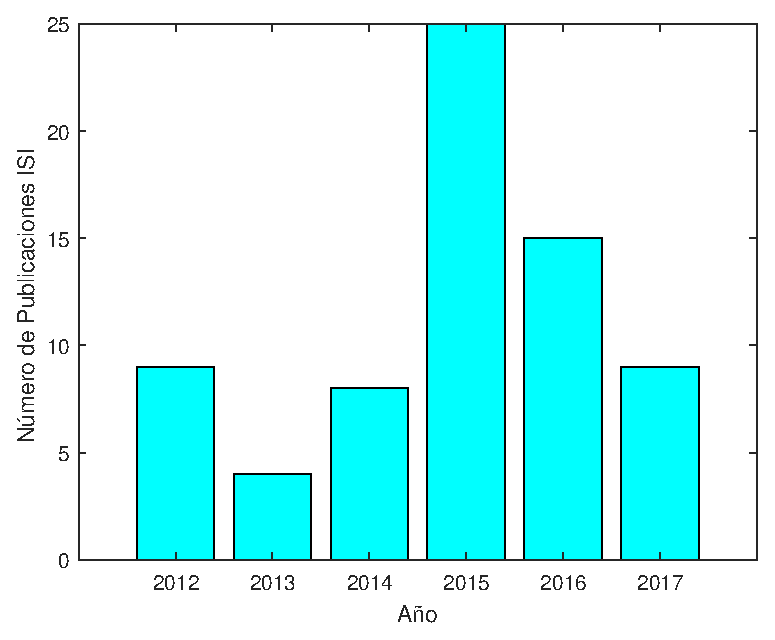
\includegraphics[width=0.7\columnwidth]{./pictures/publicaciones_ISI.eps}
\caption{Publicaciones con indexación ISI total de los profesores del claustro por año.}
\label{pub_isi}
\end{figure}

Adicionalmente en la encuesta (ver Sección \ref{academicos}) egresados y estudiantes del
Programa declaran 
estar entre muy de acuerdo y de acuerdo que el cuerpo académico
tiene una importante trayectoria, medido esto último en términos de publicaciones, participación
en proyectos, experiencia laboral y docencia. Es importante mencionar que los estudiantes evalúan a todo 
el cuerpo académico, no solo a los profesores del claustro. Lo que deja evidente el aporte de los colaboradores
al Programa.

\noindent Experiencia Laboral y Consultorías

El Programa cuenta con un claustro con bastante experiencia laboral. Los profesores del claustro
han trabajado en organizaciones como Bell Laboratories, Alcatel-Lucent, Sprint-Nextel, Nortel Networks,
Rockwell Collins, Federal Aviation Administration (FAA), People on Line, entre muchas otras organizaciones
internacionales trabajando en proyectos de telecomunicaciones. Aún con esta experiencia es importante mencionar 
el gran aporte que contribuye el cuerpo académico colaborador, donde gracias a estos profesores el Programa
reporta 30 consultas hechas en diversas organizaciones, hechas en el área de las telecomunicaciones.

\noindent Participación en Proyectos

Casi la totalidad de los miembros del claustro
lideran proyectos de investigación de forma permanente. Se destaca la participación de un 75\% del
claustro en Proyectos Fondecyt Regular e Iniciación (es decir, 3 de 4 académicos, donde los que
no tienen participación son académicos recientemente integrados). Además, los profesores mantienen numerosos
proyectos de transferencia y ciencia aplicada (Fondef, IDeA, entre otros). El total de proyectos en que participan 
los integrantes del claustro suma 26. El cuerpo académico colaborador 
también a participado en varios proyectos CORFO entre otros. 

\subsubsection{Crecimiento del Claustro e Incorporación de Académicos}

Adicionalmente a
la calidad de nuestra actividad es importante resaltar la renovación y crecimiento que ha
experimentado el claustro de Magíster en los últimos años, donde se constata la incorporación
de dos académicos en el 2017, que son Sandra Céspedes y Jinsong Wu. 
Esta política de renovación del cuerpo académico se enmarca en una plan
estratégico del Departamento de Ingeniería Eléctrica en mantener áreas balanceadas generando
las instancias administrativas formales que posibilitan la renovación del cuerpo académico. En
la actualidad se constata que un porcentaje significativo del cuerpo académico está compuesto
por académicos jóvenes (menores de 40 años), correspondiente al 50\% (2 de 4 académicos). 
Esta renovación posibilita una proyección del Programa en el mediano plazo. 


\subsubsection{Internacionalización del Cuerpo Académico}
\label{internacionalizacion}

Junto a la renovación del claustro en los últimos
años se destaca también su internacionalización. Actualmente (2017) todos los miembros 
del claustro son del extranjero, donde las nacionalidades son de los siguientes países: Venezuela,
Guatemala, Colombia y China). Cabe mencionar que dos profesores tienen ciudadanía de otros países (distintos 
a donde nacieron) y estos países son Chile y Canadá. Entre los colaboradores tenemos además la nacionalidad cubana.
Estos académicos tienen vínculos formales con instituciones extranjeras, junto con redes
de colaboración activas. Adicionalmente, todos los miembros del claustro obtuvieron
sus grados de Doctor en prestigiosas universidades internacionales (EEUU, Canadá y Korea del Sur) 
y gozan de numerosas redes de colaboración internacional.

\subsubsection{Cuerpo Académico Multidiciplinario}

Dado que el Programa tiene un perfil de egreso que incluye una gran variedad de destrezas industriales,
el cuerpo académico está incorporado por profesores que son expertos en leyes, economía, gestión de 
proyectos y de ciencias de la computación. Estos profesores permiten que el Programa pueda brindar 
conocimientos de regulación de las telecomunicaciones, análisis financieros, administración de proyectos y
temas de seguridad de redes. Esta gran diversidad de disciplinas es uno de los aspectos de los cuales
más nos enorgullece del Programa.

%\subsubsection{Consolidación de Académicos del Programa}

%En los últimos 5 años los académicos del claustro
%Pablo Estévez, Claudio Pérez, Javier Ruiz del Solar, Néstor Becerra y Martin Adams han sido
%nombrados en la más alta jerarquía académica de nuestra institución, Profesor Titular, como
%distinción a sus notables aportes a la institución en los ámbitos de formación (postgrado y
%pregrado), investigación y desarrollo. Esto constata la consolidación de los académicos con más
%experiencia en el Programa, hecho que repercute directamente en la jerarquía del cuerpo académico
%de éste y por ende en su consolidación en el tiempo. Dentro de los aportes notables de este
%grupo de académicos se destaca su importante rol en la formación de estudiantes en este Programa
%y en la formulación y ejecución de proyectos de investigación de gran envergadura de carácter
%interdisciplinario e Inter-universitario: Centro Basal AMTC, Fondap de Energía y proyecto Anillo.
%Además, los profesores Jorge Silva, Marcos Orchard, Doris Sáez y Patricio Mena han pasado de la
%jerarquía Profesor Asistente a Profesor Asociado.

%\subsubsection{Calidad y pertinencia del claustro}

%Los puntos analizados en la sección anterior dan cuenta de la calidad y pertinencia del claustro
%en virtud de los objetivos trazados en el Programa de Magíster. Se destaca una consolidación
%del claustro en el último tiempo y su renovación y proyección al mediano plazo. Se observa
%una presencia balanceada en todas las líneas de investigación que se cultivan en la disciplina de
%Ingeniera Eléctrica (Formulario de Acreditación Sección 4.2.3). Al mismo tiempo, la productividad
%creciente del claustro y la creciente participación en proyectos de investigación dan cuenta de un
%ecosistema rico en oportunidades para los estudiantes del Programa de magíster.

%\subsubsection{Evaluación del Sistema de Guías}

%Respecto al sistema de guía o seguimiento de los estudiantes, por diseño, la responsabilidad en
%primera instancia recae en la figura del profesor guía de tesis. Según el Reglamento General
%de Magíster [\ref{reg_mirc}], el Comité Académico nombra un guía desde la incorporación del estudiante
%el primer semestre. Los profesores guías están informados de los reglamentos de nuestros
%Programas, donde se estipulan entre otras cosas los objetivos, el plan de estudios, los objetivos de
%graduación, plazos y cumplimiento de compromisos formales (defensa de tesis). Adicionalmente
%a esto, el Coordinador del Programa vela por el cumplimiento del reglamento y se comunica
%directamente con los estudiantes del Programa para informar del reglamento y plazos. Se destaca
%las reuniones anuales de carácter informativo, dirigidas por el Coordinador del Programa y los
%comunicados enviados por el coordinador a los estudiantes para efectos de recordar el cumplimiento
%de plazos y obligaciones. Pese a lo anterior y en virtud de los tiempos de titulación y el análisis de
%casos donde no se ha dado cumplimiento a los plazos del Programa, se observa un espacio de mejora
%que propenda a un mejor seguimiento del progreso de los estudiantes y una mayor coordinación
%con los profesores guías de tesis.

\subsection{Definiciones Reglamentarias}

La Universidad de Chile, en su Reglamento General de Carrera Académica [\ref{reg_carrera}], establece tres
posibles Categorías Académicas:

\begin{enumerate}
\item La Categoría Académica Ordinaria, con cinco rangos consecutivos.
\item La Categoría Académica Docente, con tres rangos consecutivos.
\item La Categoría Académica Adjunta, con dos rangos.
\end{enumerate}

En particular, en el Departamento de Ingeniería Eléctrica de la Facultad de Ciencias Físicas
y Matemáticas, los académicos se encuentran adscritos a la Categoría Académica Ordinaria. De
acuerdo al Reglamento General de Carrera Académica, Artículo 6 [\ref{reg_carrera}]:

``Los académicos de la Categoría Académica Ordinaria deberán realizar docencia superior e
investigación o creación artística. Podrán, además, realizar otras de las actividades indicadas en
el artículo precedente, o una labor profesional destacada en el ámbito de su quehacer
académico.''

Adicionalmente el Reglamento General de estudios conducentes a los grados académicos de
Magíster y Doctor de la Universidad de Chile, párrafo 2, artículo 12 [\ref{reg_mag_doc}], establece que para la
creación de un Programa de magíster o doctorado:

``Cada Programa será desarrollado por un claustro conformado por académicos que cultiven las
disciplinas del Programa mediante investigación o creación artística original. El ingreso de un
académico al Claustro de un Programa será propuesto por el respectivo Comité Académico y
aprobado por el Consejo de la Escuela de Postgrado. La nómina actualizada de sus integrantes
será pública. Los académicos que integren el claustro de un Programa conducente al grado de
Magíster deberán ser profesores de cualquier carrera o categoría académica.''

Las normas básicas de la estructura, organización y administración del Programa se encuentran
estipuladas en el Reglamento General del Programa [\ref{reg_mirc}]. Es importante en este punto mencionar
que hay una nueva propuesta Reglamento General del Programa en proceso de revisión desde
el primer semestre del 2015. Adicionalmente, el Programa tiene un Reglamento Interno con
disposiciones específicas para regir el Programa dentro del marco otorgado por el Reglamento
General antes mencionado. Este reglamento es revisado periodicamente por el Comité Académico
del Programa, para ajustarlo a necesidades específicas de reglamentación interna, con el fin de
impulsar iniciativas de apoyo a los estudiantes, su seguimiento y, al mismo tiempo, facilitar la
gestión y coordinación del Programa.

\subsubsection{Del Comité Académico de Postgrado}

El Reglamento General de la Universidad de Chile [\ref{reg_mag_doc}] establece:

``El Programa constará de Comité Académico nombrado por el Director de Escuela de postgrado
de la FCFM a proposición del claustro académico del Programa, con el acuerdo del Consejo de
Escuela de la FCFM. En el mismo artículo se señala que el Comité estará conformado por al
menos tres miembros del claustro, quienes elegirán a uno de ellos como Coordinador. Será
responsabilidad del Comité gestionar los aspectos académicos del Programa, velando por el
cumplimiento de sus objetivos y por el mejoramiento continuo del Programa.''

Respecto a la gestión del Programa las funciones del Comité Académico, en concordancia con
el Reglamento General, corresponden a:

\begin{enumerate}
\item Seleccionar a los estudiantes que se incorporarán al Programa.
\item Aprobar los planes de estudios de los postulantes.
\item Nombrar a los respectivos profesores guías.
\item Aprobar al profesor guía de la tesis, propuesto por cada estudiante.
\item Proponer al Director de Escuela los integrantes de la Comisión Evaluadora de la Tesis.
\item Evaluar la calidad y originalidad del trabajo realizado y decidir si este alcanzó los
estándares requeridos para una Tesis de Magíster.
\item Elaborar un informe periódico sobre el estado del Programa, verificando el cumplimiento de
los indicadores de calidad definidos por la Facultad.
\item Cautelar que la investigación que realicen los estudiantes considere las normas y
procedimientos propios de la disciplina establecidas por los Comités de Ética respectivos
y/o reconocidos por la Universidad.
\end{enumerate}

\subsubsection{Del Ingreso, Permanencia y Evaluación del Claustro Académico}
\label{ing_perm_eval}

El Reglamento General de la Universidad de Chile [\ref{reg_mag_doc}] en su articulo 12 establece que:

``El ingreso de un académico al claustro, y su posterior permanencia, será propuesta por el Comité
Académico y aprobada por el Consejo de Escuela de Postgrado de la Facultad de Ciencias Físicas
y Matemáticas''.

La incorporación es solicitada por el académico interesado y posteriormente evaluada por el
Comité Académico en sus reuniones regulares, velando por el cumplimiento de la norma. Para
efectos de la permanencia en el claustro, el Comité evalúa anualmente el cumplimiento de los
criterios anteriormente señalados.

Adicionalmente a las disposiciones reglamentarias del Programa, los académicos del claustro
están subscritos a la carrera académica ordinaria (ver reglamento general de carrera académica
[\ref{reg_carrera}]). En este marco existen procesos permanentes de Calificación Académica, donde se
evalúa el desempeño general del académico considerando para ello docencia de pre y post grado,
investigación, tutoría de estudiantes, formación de profesionales y graduados, proyectos, gestión
docente, apoyo administrativo. Este proceso se ejecuta cada dos años para profesor de la jerarquía
de Profesor Asistentes y Asociados, y cada cuatro años para la jerarquía de Profesor Titular. Este
proceso exige que los académicos garanticen un buen cumplimiento en sus actividades académicas
y es un mecanismo formal a nivel institucional para evaluar a los académicos y condicionar su
permanencia en la institución en el caso que los criterios de permanencia mínimos exigidos en la
carrera académica ordinaria no sean satisfechos.

Complementando el punto anterior, en la Universidad de Chile hay un proceso de evaluación
académica que permite el paso de jerarquía académica (ver Reglamento Consejo Evaluación
[\ref{reg_cons_eval}]). Para ello los académicos deben cumplir con estrictos estándares de desempeño en lo
que respecta a la investigación y docencia, fundamentalmente. En este marco se estipula un tiempo
máximo de permanencia en la jerarquía de profesor asistente, que es de 10 años. Este tiempo
máximo de permanencia orienta la actividad de los profesores asistentes con miras a cumplir
estándares académicos que les permitan llegar a la jerarquía de Profesor Asociado en el plazo
señalado. Este proceso busca que los académicos pongan prioridad en actividades de investigación
y docencia de postgrado, de tal forma de mostrar independencia académica, liderar proyectos de
investigación como investigadores principales, y formar nuevas generaciones de profesionales y
académicos que cultiven su área del conocimiento.

\subsubsection{De la dedicación del claustro académico}

Como se explicó en la Sección \ref{ing_perm_eval}, los miembros
del claustro deben estar suscritos a la carrera académica ordinaria en el grado de profesor asistente,
asociado o titular. Por tanto todos los miembros del claustro tienen una dedicación de tiempo
completo a sus quehaceres académicos y docentes dentro de la universidad.

\subsubsection{Del sistema guías}

En concordancia con el reglamento general [\ref{reg_mag_doc}] en su artículo 26, al momento del ingreso del
estudiante al Programa la coordinación define su guía entre los académicos del claustro. Este
cumple el rol de orientar al estudiante en sus actividades académicas. Adicionalmente, para la
ejecución de la tesis el estudiante constará con un profesor guía de tesis nombrado por el Comité
Académico del Programa a proposición del estudiante, en concordancia con lo que establece el
Artículo 28 del mismo reglamento. El profesor guía de tesis debe pertenecer al claustro académico
del Programa.

\subsubsection{Evaluación docente}

Como parte de una política institucional de la FCFM, a través de la plataforma de U-Cursos, todos
los cursos cuentan con una encuesta para la evaluación docente de los profesores que se realiza
dos veces al semestre. Los resultados de esta evaluación son analizados en primera instancia por la
Jefatura Docente donde se determina si se debe ofrecer ayuda al profesor para la preparación del
curso junto con el área el departamento ADD. Por otro lado, los resultados de la encuesta forman
parte de todos los procesos de evaluación y cambio de jerarquía descritos en la Sección 2.4.3.2.

El sistema de profesores guías es evaluado en encuestas que se realizan previos al
proceso de acreditación. Una evaluación más rutinaria es necesaria. En la encuesta se observa que
la calificación dada por los estudiantes del Programa a sus profesores guías es
sobresaliente (ver Sección \ref{academicos}).

Un espacio de mejora en lo que refiere a tener información del desempeño de los profesores
guías de tesis, es hacer un evaluación más sistemática como se declara en el Plan de
Desarrollo de este proceso.

\subsubsection{Del seguimiento de los estudiantes}

El seguimiento de los estudiantes es una parte imprescindibles para la formación completa de los estudiantes. Como parte 
del seguimiento se tratan de detectar las debilidades en los conocimientos de los estudiantes en forma individual. A los 
estudiantes que exhiben debilidades se les trata de apoyar con distintos medios, por ejemplo: revisar las debilidades en 
la oficina del profesor, revisar las respuestas de las pruebas en la sala de clases, asignar tareas adicionales para que 
el estudiante practique, entre otros medios. La revisión de las pruebas luego de la examinación es beneficiosa tanto para 
los estudiantes de demostraron debilidades, tanto como para aquellos que mostraron dominio de los conceptos, ya que en este 
último caso la revisión de los resultados refuerza los conocimientos.

\section{Recursos de Apoyo}

\subsection{Apoyo Institucional e Infraestructura}
\label{apoyo_inst}

\subsubsection{Laboratorios y equipamiento}

El Programa cuenta con una amplia gama de laboratorios para la formación de sus estudiantes.
Efectivamente, el Departamento de Ingeniería Eléctrica posee tanto laboratorios docentes como de
investigación. Existen ocho laboratorios docentes especializados en diversos temas de ingeniería
eléctrica (ver detalles en Sección 5.1.2 del Formulario de Antecedentes del Programa):

\begin{itemize}
\item Laboratorio de Electricidad Básica,
\item Laboratorio de Automática,
\item Laboratorio de Accionamiento,
\item Energía y Electrónica de Potencia,
\item Laboratorio de Mecatrónica,
\item Laboratorio de Sistemas Inteligentes,
\item Laboratorio de Telecomunicaciones,
\item Laboratorio de Máquinas Eléctricas y
\item Laboratorio de Electrónica.
\end{itemize}

Estos son utilizados por los alumnos de pregrado y postgrado para completar su formación teórica.
Por otro lado existen 15 laboratorios de investigación donde estudiantes de pre y postgrado
realizan investigación:

\begin{itemize}
\item Laboratorio de Acumuladores,
\item Laboratorio de Control Avanzado,
\item Laboratorio de Energía y Accionamientos,
\item Laboratorio de Información y Decisión,
\item Laboratorio de Ingeniería Biomédica,
\item Laboratorio de Inteligencia Computacional,
\item Laboratorio de Micro Redes y Electromovilidad,
\item Laboratorio de Ondas Milimétricas y Submilimétricas,
\item Laboratorio de Procesamiento y Transmisión de Voz,
\item Laboratorio de Robótica, Laboratorio de Fotónica,
\item Optical \& Wireless Laboratory,
\item Laboratorio de Procesamiento Digital de Imágenes,
\item Laboratorio de Visión Computacional y
\item Laboratorio de Exploración Espacial y Planetaria.
\end{itemize}

En estos últimos los estudiantes de postgrado realizan la investigación y desarrollo relacionada a su trabajo
de tesis (Una descripción detallada de los laboratorios puede consultarse en el Formulario de
Acreditación Sección 5.1).

Todos los laboratorios cuentan con un responsable técnico y cuentan con un equipamiento
adecuado y en crecimiento. Las FCFM y el DIE garantizan la infraestructura básica de todos los
laboratorios. El financiamiento para la mantención y adquisición de nuevo equipamiento de los
laboratorios docentes es responsabilidad de la FCFM y del DIE. En el caso de los laboratorios
de investigación esta responsabilidad recae en el profesor o profesores líderes de cada laboratorio,
quienes recurren a fondos concursables.

\subsubsection{Recursos Bibliográficos}

Los estudiantes tienen acceso a una importante colección de recursos bibliográficos a través del
sistema de Bibliotecas de la Universidad10. Físicamente, se puede acceder a más de 120000 libros.
Además, a través de una moderna página web, se puede acceder electrónicamente a colecciones
de libros y revistas de conocidas casas editoriales. En particular, el DIE financia el acceso a la
colección de revistas de la IEEE, la más importante casa editorial de revistas científicas en diversas
áreas de la ingeniería eléctrica11. Respecto a las áreas más cercanas de investigación del Programa
podemos mencionar las siguientes subscripciones a revistas:

\begin{itemize}
\item 762 en Ingeniería Eléctrica en sí misma. En particular existe acceso a todas las revistas de
IEEE,
\item 145 en Tecnología de la Información,
\item 311 en Telecomunicaciones,
\item 118 en Física Aplicada,
\item 309 en Tecnología en General y
\item 111 en Astronomía y Astrofísica.
\end{itemize}

%\subsubsection{Becas y Ayudas de Viaje}

%En la actualidad el Programa cuenta con una rebaja arancelaria que equipara el arancel del
%Programa al fijado por Conicyt para sus becarios (actualmente \$1.000.000). Esta rebaja
%corresponde a un porcentaje importante del arancel anual del Programa. Este apoyo busca generar
%las condiciones favorables para que estudiantes que están participando en calidad de tesistas de un
%proyecto formal de investigación puedan pagar un arancel sustancialmente más bajo y por ende es
%un instrumento de apoyo a los estudiantes del Programa. Para esta ayuda se requiere autorización
%del tutor o profesor guía de tésis, quien solicita formalmente la ayuda al coordinador del Programa.

%En cuanto a las ayudas de viaje, esta es una dimensión donde se pueden hacer esfuerzos
%adicionales por mejorar. En el Plan de Desarrollo del presente proceso se elabora una nueva política
%para apoyar la participación de estudiantes del Programa en Congresos Internacionales. El criterio
%es que la conferencia sea de nivel mundial en su área de interés y que el estudiante presente un
%trabajo en calidad de primer autor. Este instrumento se comenzó a ejecutar el presente año 2015
%(ya se han hecho dos llamados a la fecha) y ha sido positivamente evaluado por los estudiantes
%activos del Programa como se constata en el ítem 7 de la encuesta (3.4.1).

\subsubsection{Vinculación con el Medio}
\label{vinculacion_medio}

El Programa tiene un vínculo con el medio a través de la investigación. Existen colaboraciones 
con científicos y organizaciones extranjeras a través de distintos proyectos e iniciativas. 
Un ejemplo de vinculación con el medio que se destaca es la colaboración 
que existe a través del proyecto ERANet-LAC. En este proyecto participan instituciones de 4 países de 
Latinoamérica y Europa. Los países que participan en este proyecto, a parte de Chile, son México,
Letonia y Romania.

Otra iniciativa internacional en que participaron todos los miembros del claustro y muchos colaboradores del Programa
fue una iniciativa llamada FOKUS, liderada por una organización alemana en Berlín, que tuvo participación de instituciones
académicas localizadas en Alemania, China y Tailandia, a parte de Chile.

Actualmente la Facultad cuenta con varios centros (mencionados en la Sección \ref{estruct_org_fcfm}) y 8 unidades de investigación
avanzada. A través de estos se realizan actividades de vinculación
con el sector productivo y la sociedad, con énfasis en la creación de conocimiento, desarrollo
y transferencia tecnológica. Cada uno es líder en su disciplina en el país. De estos centros
destacamos a continuación dos que son liderados por académicos del DIE y donde estudiantes del Magíster en Ingeniería de Redes de Comunicaciones ya han 
participado y donde otros tienen la oportunidad de participar.

\begin{itemize}
\item Centro Avanzado de Tecnología para la Minería (AMTC), Director: Dr. Javier Ruiz Del
Solar (DIE)
\item Centro de Investigaciones en Energía Solar (SERC-Chile), Director: Dr. Rodrigo Palma
Behnke (DIE)
\end{itemize}

Además, de todos estos vínculos también existen canales de colaboración con empresas como Entel
(en particular su rama de innovación), Telefónica I+D, 
Zweicom, ZTE Chile y ESIMTEL. Además de tener una buena relación con estas 
empresas, también han existido instancias de colaboración formal en proyectos FONDEF y CORFO.


\section{Capacidad de Autorregulación}

\subsection{Equilibrio entre estudiantes y recursos}

El Programa se ha caracterizado por velar por un adecuado equilibrio entre el número de estudiantes
matriculados y los recursos existentes. Prueba de ello es la consolidación del cuerpo académico. El
claustro del Magíster en Ingeniería de Redes de Comunicaciones, corresponde actualmente a
13 profesores contando los mismos del claustro y colaboradores. La cantidad de estudiantes 
activos en el Programa es de 13, lo que da una
razón promedio de 1 estudiantes por profesor. Esto es coherente con el hecho de que este es
un Programa orientado al desarrollo de competencias complejas en nuestros egresados, donde la
interacción personalizada con el profesor guía es esencial para lograr los objetivos del perfil
de egreso declarado.

Respecto a los recursos del Programa, en términos de laboratorios, biblioteca,
recursos bibliográficos, espacios de estudios, entre otros, éstos se caracterizan por su calidad
como se puede ver en detalle en la Sección \ref{apoyo_inst} de este informe. Como evidencia, la encuesta
a egresados, estudiantes y académicos muestra un amplio consenso respecto a la calidad del
Programa en lo que respecta a Apoyo Institucional e Infraestructura (ver Sección \ref{apoyo_inst_infra}). Sin
embargo, se aprecia un gran espacio de mejora en lo que respecta a laboratorios y/o talleres docentes
y la idoneidad de salas de clases para cumplir los requerimientos académicos. Cabe mencionar que se 
ha tenido dificultades con el equipo audiovisual (específicamente proyectores), probablemente 
debido a su extenso y constante uso, donde ha fallado en varias ocasiones. Se ha remplazado el equipo en al menos 
3 ocasiones en un periodo de 4 años. Es necesario estudiar el remplazo de estos equipos por una alternativa más duradera.
Esta ha sido una situación recurrente en el Programa.

En línea con el mejoramiento del Programa, es necesario tener mejoras con respecto al apoyo de
pasantías, congresos y otras actividades. A pesar de que el objetivo del Programa, ni el plan de
estudio exigen este tipo de actividades, sería idóneo poder financiarlos. Hay que estudiar bien 
la metodología, beneficios, recursos existentes y otros factores antes de ejecutar un plan 
(más detalles en el Plan de Desarrollo en la Sección \ref{plan_de_desarrollo}).

\subsection{Difusión}

La Universidad de Chile es particularmente cuidadosa en toda la entrega de información referente
a sus carreras y Programas de postgrado. En lo que se refiere a la difusión del Programa, se puede
mencionar la pagina web del DIE y MIRC como una plataforma con la información relevante del
Programa, su cuerpo académicos y otra informacióm importante. 
Acorde con esta política se han Programado visitas a universidades en la región al mismo modo que
solicitado a cada miembro del claustro del Programa que difunda el Programa en las conferencias y
seminarios internacionales en los que le toca participar regularmente. Otra instancia de difusión, es nuestra 
carta de presentación, o sea, nuestros egresados, que en un alto porcentaje declaran que recomendarían
el Programa a sus colegas y están satisfechos con la formación recibida del Programa.
Lo anterior se ve evidenciado por la alta apreciación y evaluación del Programa recogida en las
encuestas a egresados. % (ver Sección 3.4.1.9).

Complementariamente, parte de los esfuerzos de difusión del Programa son canalizados por
los medios oficiales de la Universidad de Chile a nivel de la Escuela de Postgrado y la Facultad.
En esto último, hay variadas actividades de difusión del quehacer de la Facultad donde se destacan
los días de puertas abiertas, la organización de charlas y seminarios, la publicación de la revista
Beaucheff, la página web de la Facultad y la Escuela de Postgrado. Es importante mencionar que
existe una unidad encargada de la difusión en la Facultad con recursos disponibles, Programas de
acción y personal administrativo dedicado a dichas tareas. En todos estos medios institucionales el
Departamento de Ingeniería Eléctrica ha mostrado una activa visibilidad. Actualmente la Escuela
de Postgrado realiza giras en Latinoamérica realizando difusión de toda la oferta de Postgrados de
la Facultad.

\subsection{Reglamentación}

La estructura reglamentaria de la Universidad de Chile es clara en lo que respecta a los Programas
conducentes a los grados de magister y doctorado [\ref{reg_mag_doc}]. Esta reglamentación define un marco
sobre el cual se regulan los Programas tocando aspectos tales como la naturaleza del Programa,
sus objetivos y perfil de graduación, su creación, la administración, la conformación del claustro,
las responsabilidades del comité académico, las responsabilidades de la escuela de postgrado, la
acreditación y procesos de aseguramiento de calidad. Adicionalmente en este Reglamento hay
disposiciones especificas para los Programas de Magister que tocan aspectos relativos a postulación
y criterios de selección, plan de formación, proyecto de grado, actividad de graduación, extensión
mínima y máxima del Programa, homologación de UDs, criterios de aprobación, entre otros.
Complementando lo anterior, el Programa mantiene un Reglamento General [\ref{reg_mirc}]. El Reglamento General del
Programa fue aprobado el 2016.


\subsection{Difusión de la Reglamentación}

Los reglamentos son públicos y de libre disposición para todos los miembros del Programa
(estudiantes y académicos). En particular, la pagina web del DIE mantiene dicha información
vigente. Sin embargo, el plan de desarrollo considera mejoras en este aspecto.

\subsection{Procesos de Diagnóstico}

El mejoramiento continuo y las instancias de diagnóstico se entienden como una parte esencial de
los Programas de postgrado que imparte la Universidad de Chile. En este marco, el Reglamento
General de la Universidad de Chile establece que los procesos de autoevaluación son parte esencial
de las responsabilidades del Comité Académico del Programa. Se establece que estos procesos
deben ser continuos y debe haber un proceso formal de revisión al menos cada 5 años. En
este contexto en los últimos años ha habido una serie de actividades e iniciativas de análisis y
diagnóstico participativas: Jornada de Escuela de Postgrado, Jornada estratégicas departamental
(Departamento de Ingeniería Eléctrica), análisis y revisión de los reglamentos del Programa,
reuniones con el claustro, así como las constantes reuniones del Comité Académico donde se
discuten aspectos operativos y estratégicos del Programa. A esto se suma el presente proceso de
autoevaluación del Programa. Adicionalmente el Programa consta con instrumentos de diagnóstico
que son utilizados regularmente para evaluarlo como son las Encuesta Docentes y el seguimiento
académico de sus estudiantes a través de la plataforma U-campus.

En el presente proceso, nuevas medidas han sido contempladas para el Plan de Desarrollo
donde se destaca la elaboración y toma de encuesta a la salida a los graduados del Programa y
la generación de informes anuales con indicadores que midan el desempeño del Programa. La
generación de estos insumos es importante para el análisis del Programa y con ello el desarrollo
futuro de éste.

\subsection{Plan de Desarrollo}

La elaboración y ejecución del plan de desarrollo se encuentra a cargo del Comité Académico
del Programa, liderado por su coordinador (artículo 17 Reglamento General [\ref{reg_mag_doc}]). Los recursos
para su ejecución provienen de recursos del Programa y del Departamento de Ingeniería Eléctrica.
En la ejecución del plan, el Comité recibe apoyo del equipo de gestión docente (jefe de estudios
y secretaria de postgrado). El plan de desarrollo que se desprende del presente proceso de
acreditación se presenta en forma detallada en el Capítulo 3 del presente informe.

\subsection{Autoevaluación y mejoramiento continuo}

Como se ha mencionado en el punto anterior, la Universidad de Chile es una institución fuertemente
autorregulada, dinámica y en mejora constante. Esto queda de manifiesto en las continuas mejoras
en todos los niveles institucionales y en diferentes dimensiones. Para mencionar algunas de las
instancias formales donde se generan los espacios de análisis y discusión de los Programas se
mencionan los procesos de autoevaluación, jornadas de análisis de postgrado a nivel institucional y
departamental, reuniones regulares del comité académico del Programa, procesos de actualización
periódica de los reglamentos, perfeccionamiento de instancias centrales como la Escuela de
Postgrado.


%----------------------------------------------------------------------------------------
%	CHAPTER 3
%----------------------------------------------------------------------------------------

\chapterimage{sintesis.jpg}
\chapter{Síntesis del Proceso de Autoevaluación}
\section{Organización}

Para enfrentar el actual proceso de acreditación, el Comité Académico del Programa constituyó un
comité ad hoc dedicado a llevar a cabo el presente proceso de autoevaluación. Este comité cuenta
con el apoyo del Departamento de Ingeniería Eléctrica en términos administrativos y financieros.

La Figura 3.1 muestra el organigrama de dicho equipo y está integrado por:

\begin{itemize}
\item Coordinador de Acreditación: Claudio Estévez, Coordinador del Programa, Profesor Asistente.
\item Comité de Acreditación
\begin{itemize}
\item Claudio Estévez, Coordinador del Programa, Profesor Asistente
\item Álvaro Silva, Profesor Colaborador.
\end{itemize}
\item Comité Académico:
\begin{itemize}
\item Claudio Estévez, Coordinador del Programa, Profesor Asistente.
\item César Azurdia, Profesor Asistente
\item Sandra Céspedes, Profesora Asistente
\end{itemize}
\item Equipo Ejecutivo:
\begin{itemize}
\item Jhilmar Molina, Ingeniero Civil Eléctrico.
\item Jorge Flores, Ingeniero Civil Eléctrico.
\item Andrea Canales, Ingeniera Civil Industrial.
\end{itemize}
\item Claustro.
\item Estudiantes del Programa.
\item Egresados del Programa.
\item Institucionalidad:
\begin{itemize}
\item Dirección de Postgrado y Postítulo.
\item Escuela de Postgrado.
\item Otras Direcciones y Escuelas.
\end{itemize}
\end{itemize}

% Figura 3.1

\section{Participación}

Se ha definido el proceso como altamente participativo, en cada etapa se ha considerado la
participación e iteración de los distintos estamentos indicados anteriormente.

\begin{itemize}
\item Se realizó una reunión con las autoridades de la Escuela de Postgrado para dar inicio formal al proceso de autoevaluación.
\item Se realizó una reunión con el Comité Académico para discutir el proceso de acreditación.
\item El comité de acreditación trabajó en forma individual y se reunió en varias ocasiones para discutir el progreso.
\item Se realizaron jornadas informativas donde participó todo el cuerpo académico del Programa.
\item Se informó a los estudiantes activos del Programa que este se estaba acreditando y solicitaba su ayuda y retroalimentación.
\item Se informó a los egresados del Programa que este se estaba acreditando y solicitaba su ayuda y retroalimentación.
\item Se realizaron jornadas de discusión para elaborar el plan de desarrollo con el cuerpo académico del Programa, liderado por el Comité de Acreditación.
\item Se revisa el documento final por todo el cuerpo académico del Programa, recogiendo sugerencias y comentarios.
\end{itemize}


Jornadas participativas:

\begin{itemize}
\item Equipo Acreditación
\item Comité Académico del Programa
\item Claustro
\item Colaboradores
\item Estudiantes del Programa
\end{itemize}

En estas jornadas se presentó la información recabada a lo largo del proceso así como la información consolidada de las encuestas.

\section{Encuestas Acreditación}
\label{encuestas}

El equipo de acreditación en conjunto con la escuela de Postgrado desarrollaron y aplicaron
encuestas a estudiantes, graduados y académicos del Programa. Esto con la finalidad de enriquecer
la autoevaluación e identificar fortalezas y debilidades del Programa. Se presentan a continuación
los resultados más relevantes\footnote{El detalle de las encuestas se encuentra en los anexos y encuestas individuales [\ref{enc_det}]}.

\section{Criterio de Análisis}
\label{criterio_analisis}

Para analizar las encuestas en forma metodológica y objetiva se decide establecer un criterio para
establacer qué aspectos son fortalezas y debilidades. El primer paso es mapear las respuestas a una nota numérica,
como se puede ver en la Tabla \ref{criterio_mapa}. Luego se definen las notas que se consideran fortalezas y debilidades. 
También se ha decidido tener un rango que llamamos ``oportunidad de mejora'', donde el aspecto evaluado 
no se considera como fortaleza o debilidad, sino un punto intermedio. Para efectos del Plan de Desarrollo los aspectos 
que se consideren oportunidades de mejora son como debilidades pero con una prioridad más baja. Las definiciones
de los rangos de las notas se pueden observar en la Tabla \ref{criterio_definicion} y visualmente 
en la Figura \ref{criterios_fig}. Vale la pena mencionar 
que el umbral entre ``De acuerdo'' y ``En desacuerdo'' se encuentra en 2,5. Por este motivo determinamos que los aspectos
que estén en el rango entre 
este umbral (2,5) y la nota mínima (1) se consideran debilidades y del mismo umbral (2,5) hasta la nota 
de ``De acuerdo'' (3) es una oportunidad de mejora. Solo si la nota promedio cae entre ``De acuerdo'' y
``Muy de acuerdo'' se considera una fortaleza. 

\begin{remark} 
Es muy importante destacar que el objetivo del Programa es mejorar en todos los aspectos. Esta medida de categorización es un ejercicio 
para identificar las aspectos que requieren una mejora urgente (debilidades) que se abordarán con alta prioridad y aspectos débiles pero a menor grado (oportunidad de mejora) que se mejorarán con una prioridad secundaria. Incluso, se planea mejorar las fortalezas, pero con una prioridad más baja.
\end{remark}


\begin{table}[!ht]
\centering
\caption{Mapeo de respuesta a notas.}
\label{criterio_mapa}
\begin{tabular}{lc}
\hline
Selección         & Nota \\ \hline \hline
Muy de acuerdo    & 4    \\
De acuerdo        & 3    \\
En desacuerdo     & 2    \\
Muy en desacuerdo & 1    \\
\hline
\end{tabular}
\end{table}

\begin{table}[!ht]
\centering
\caption{Definiciones de fortaleza, debilidad y oportunidad de mejora.}
\label{criterio_definicion}
\begin{tabular}{lc}
\hline
Categoría             & Rango de Notas \\ \hline \hline
Fortaleza             & {[}4 , 3{]}    \\ 
Oportunidad de Mejora & (3 , 2,5{]}    \\ 
Debilidad             & (2,5 , 0{]}    \\ \hline
\end{tabular}
\end{table}

\begin{figure}[!ht]
\centering
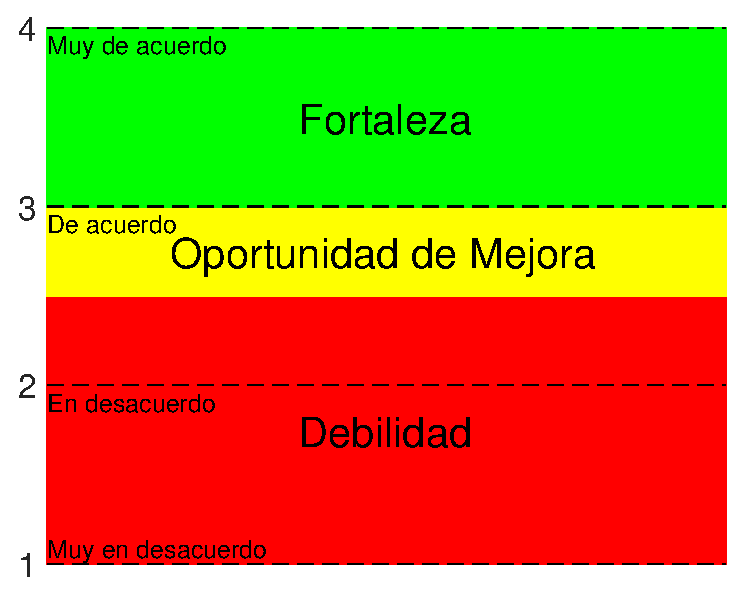
\includegraphics[width=0.5\columnwidth]{./pictures/criterios.eps}
\caption{Definiciones de rango de notas para las categorías de Fortaleza, Debilidad y Oportunidad de Mejora.}
\label{criterios_fig}
\end{figure}




\subsection{Consolidado de las Encuestas}

Primero se presenta un resumen de las estadísticas, de forma que sea fácil de ver donde se 
presentan los problemas más grandes. Utilizando el sistema de notas descrito en la sección previa obtenemos 
los promedios de las distintas categorías por grupo, siendo los grupos: Académicos, Egresados y Estudiantes. 
Estos resultados me muestran en la Figura \ref{encuestas_fig}. Los puntos que corresponden a "Total", 
representan los promedios ponderados (considerando la cantidad de personas que contestaron por grupo) de cada 
categoría. La categoría de Egresados corresponde a preguntas que solo fueron hechas al grupo de los egresados,
por lo que su promedio es el mismo valor y no se graficó. Debajo de la Figura \ref{encuestas_fig} se puede observar
lo que significan los acrónimos del eje horizontal.

Esta vista general muestra que los aspectos que más presentan debilidades son el Apoyo Institucional e Infraestructura (AII) y
la Vinculación con el Medio (VM). Las fortalezas más importantes corresponden a los aspectos de Requisitos de Admisión y 
Proceso de Selección (RAPS), Estructura del Programa y Plan de Estudios (EPPE) y Académicos (Acad). También se puede 
observar que los egresados evaluaron bastante bien el Programa, con casi todos los aspectos entre Muy de acuerdo y De acuerdo.




\begin{figure}[!ht]
\centering
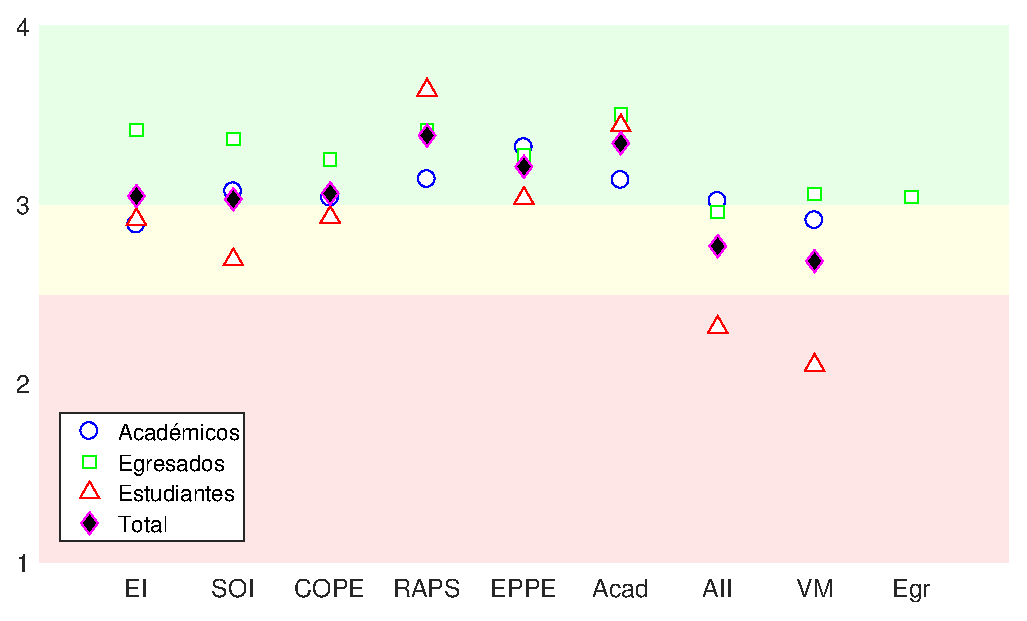
\includegraphics[width=0.8\columnwidth]{./pictures/encuestas.eps}
\caption{Resumen de las encuestas por categoría.}
\label{encuestas_fig}
\end{figure}

\begin{table}[!ht]
\centering
\label{acronyms}
\begin{tabular}{rl}
EI   & Entorno Institucional                         \\
SOI  & Sistema de Organización Interna               \\
COPE & Carácter, Objetivos y Perfil de Egreso        \\
RAPS & Requisitos de Admisión y Proceso de Selección \\
EPPE & Estructura del Programa y Plan de Estudios    \\
Acad & Académicos                                    \\
AII  & Apoyo Institucional e Infraestructura         \\
VM   & Vinculación con el Medio                      \\
Egr  & Egresados                                    
\end{tabular}
\end{table}

\begin{table}[!ht]
\centering
\caption{Información sobre la representatividad de los datos recolectados de las encuestas.}
\label{representatividad_encuestas}
\begin{tabular}{lccc}
\hline
Grupo       & Contestaron & Total & Porcentaje \\ \hline \hline
Académicos  & 8 & 13 & 61,5\% \\
Egresados   & 6 & 8 & 75\% \\
Estudiantes & 7 & 11 & 63,6\% \\
\hline
\end{tabular}
\end{table}


El detalle de cada categoría se presenta en las siguientes secciones. Presentamos los datos en el mismo orden de la encuesta.



\subsubsection{Entorno Institucional}

\noindent\textbf{General}

En el caso del Entorno Institucional (EI), las notas promedio de los 
académicos es de 2,89, de los egresados es de 3,42 
y de los estudiantes es de 2,92, generando el total de 3,05.
Esto indica que esta categoría, en general, es una fortaleza del Programa. Sin embargo, hay aspectos individuales 
que se deben mejorar. 

\noindent\textbf{Individual}

A continuación se enlistan los casos que presentan oportunidades de mejora y debilidades en base a los resultados de la Tabla \ref{entorno_institucional}.

\noindent\textbf{Oportunidades de Mejora:}

\begin{itemize}
\item La normativa que regula el programa de postgrado es clara y conocida
\end{itemize}


\begin{table}[!ht]
\centering
\caption{Resultados encuesta acerca de entorno institucional.}
\label{entorno_institucional}
\begin{tabular}{p{6.2cm}cccc}
\hline
\multicolumn{5}{r}{Promedio de las Encuestas [1-4](4 es mejor o ``Muy de acuerdo'')} \\ \cline{2-5} 
& Académicos  & Egresados & Estudiantes & Total \\
\hline \hline
\begin{tabular}[c]{@{}p{6cm}@{}}La normativa que regula el programa de postgrado es clara y conocida\end{tabular} & 2,63 & 3,33 & 2,83 & 2,9 \\
\hline
\begin{tabular}[c]{@{}p{6cm}@{}}El plan de formación del programa es conocido por los académicos/egresados/estudiantes\end{tabular} & 3,14 & 3,5 & 3 & 3,2 \\ \hline
\end{tabular}
\end{table}


\subsubsection{Sistema de Organización Interna}

\noindent\textbf{General}

En el caso del Sistema de Organización Interna (SOI), las notas promedio de los 
académicos es de 3,07, de los egresados es de 3,37 
y de los estudiantes es de 2,69, generando el total de 3,03.
Esto indica que esta categoría, en general, es una fortaleza del Programa. Sin embargo, hay aspectos individuales 
que se deben mejorar. 

\noindent\textbf{Individual}

A continuación se enlistan los casos que presentan oportunidades de mejora y debilidades en base a los resultados de la Tabla \ref{org_interna}.

\noindent\textbf{Oportunidades de Mejora:}

\begin{itemize}
\item En general, el programa funciona de manera eficiente y ordenada en términos académicos
\item Existen actividades que permiten la coordinación entre los académicos del programa
\end{itemize}

\noindent\textbf{Debilidad:}

\begin{itemize}
\item Se hace un buen seguimiento de los estudiantes
\end{itemize}


\begin{table}[!ht]
\centering
\caption{Resultados encuesta acerca del sistema de organización interna.}
\label{org_interna}
\begin{tabular}{p{6.2cm}cccc}
\hline
\multicolumn{5}{r}{Promedio de las Encuestas [1-4](4 es mejor o ``Muy de acuerdo'')} \\ \cline{2-5} 
& Académicos & Egresados & Estudiantes & Total \\
\hline \hline
\begin{tabular}[c]{@{}p{6cm}@{}}En general, el programa funciona de manera eficiente y ordenada en términos académicos\end{tabular} & 2,86 & 3 & 2,43 & 2,76  \\
\hline
\begin{tabular}[c]{@{}p{6cm}@{}}Cuando tengo un problema siempre recibo la orientación e información adecuada para resolverlo\end{tabular} & 3,43 & 3,33 & 2,57 & 3,11 \\ 
\hline
\begin{tabular}[c]{@{}p{6cm}@{}}Existen actividades que permiten la coordinación entre los académicos del programa\end{tabular} & 2,5 & N/A & N/A  & 2,5 \\
\hline
\begin{tabular}[c]{@{}p{6cm}@{}}En general, la organización administrativa (toma de asignaturas, solicitudes de certificados, etc.) del programa funciona de manera eficiente\end{tabular} & N/A & 3,5 & 2,71 & 3,07  \\
\hline
\begin{tabular}[c]{@{}p{6cm}@{}}Existen instancias de participación de los académicos para la toma de decisiones en temas relevantes del programa (malla curricular, sistemas de evaluación, otros)\end{tabular} & 3 & N/A & N/A & 3 \\ 
\hline
\begin{tabular}[c]{@{}p{6cm}@{}}Los mecanismos para comunicarse con docentes y autoridades eran conocidos por los estudiantes\end{tabular} & N/A & 3,5 & 3,14 & 3,31 \\ 
\hline
\begin{tabular}[c]{@{}p{6cm}@{}}Los canales para comunicarse con los estudiantes son los adecuados\end{tabular} & 3,57 & 3,5 & 3,29  & 3,46 \\
\hline
\begin{tabular}[c]{@{}p{6cm}@{}}Se hace un buen seguimiento de los estudiantes\end{tabular} & N/A & N/A & 2 & 2\\
\hline
\end{tabular}
\end{table}



\subsubsection{Carácter, Objetivos y Perfil de Egreso}
\label{caract_obj_perf_egr}

\noindent\textbf{General}

En el caso del Carácter, Objetivos y Perfil de Egreso (COPE), las notas promedio de los 
académicos es de 3,04, de los egresados es de 3,25 
y de los estudiantes es de 2,93, generando el total de 3,06.
Esto indica que esta categoría, en general, es una fortaleza del Programa. Sin embargo, hay aspectos individuales 
que se deben mejorar. 

\noindent\textbf{Individual}

A continuación se enlistan los casos que presentan oportunidades de mejora y debilidades en base a los resultados de la Tabla \ref{obj_y_perfil}.

\noindent\textbf{Oportunidades de Mejora:}

\begin{itemize}
\item El perfil de graduación del programa es conocido por los académicos
\item El perfil de egreso logra dar cuenta de los objetivos del programa
\end{itemize}


\begin{table}[!ht]
\centering
\caption{Resultados encuesta acerca del Carácter, Objetivos y Perfil de Egreso del Programa.}
\label{obj_y_perfil}
\begin{tabular}{p{6.2cm}cccc}
\hline
\multicolumn{5}{r}{Promedio de las Encuestas [1-4](4 es mejor o ``Muy de acuerdo'')} \\ \cline{2-5} 
& Académicos & Egresados & Estudiantes & Total \\
\hline \hline
\begin{tabular}[c]{@{}p{6cm}@{}}El programa tiene objetivos claros y conocidos\end{tabular} & 3,25 & 3,33 & 2,71 & 3,09  \\
\hline
\begin{tabular}[c]{@{}p{6cm}@{}}Los objetivos son congruentes con el enfoque del programa\end{tabular} & 3,13 & 3,17 & 2,71 & 3 \\ 
\hline
\begin{tabular}[c]{@{}p{6cm}@{}}El perfil de graduación del programa es conocido por los académicos/egresados/estudiantes\end{tabular} & 2,63 & 3,33 & 3 & 2,95  \\
\hline
\begin{tabular}[c]{@{}p{6cm}@{}}El programa tiene un perfil de graduación claro\end{tabular} & 3 & 3,17 & 2,86 & 3 \\ 
\hline
\begin{tabular}[c]{@{}p{6cm}@{}}El perfil de egreso logra dar cuenta de los objetivos del programa\end{tabular} & 3,17 & 2,83 & 2,86  & 2,97 \\
\hline
\begin{tabular}[c]{@{}p{6cm}@{}}Tengo conocimiento acerca de si la orientación del programa es de tipo profesional o académico\end{tabular} & N/A & 3,67 & 3,43  & 3,54 \\
\hline
\end{tabular}
\end{table}



\subsubsection{Requisitos de Admisión y Proceso de Selección}

\noindent\textbf{General}

En el caso del Requisitos de Admisión y Proceso de Selección (RAPS), las notas promedio de los 
académicos es de 3,14, de los egresados es de 3,42 
y de los estudiantes es de 3,64, generando el total de 3,39.
Esto indica que esta categoría, en general, es una fortaleza del Programa. 

\noindent\textbf{Individual}

Ningún aspecto individual presenta debilidades.


\begin{table}[!ht]
\centering
\caption{Resultados encuesta acerca de los requisitos de admisión y proceso de selección.}
\label{admision}
\begin{tabular}{p{6.2cm}cccc}
\hline
\multicolumn{5}{r}{Promedio de las Encuestas [1-4](4 es mejor o ``Muy de acuerdo'')} \\ \cline{2-5} 
& Académicos & Egresados & Estudiantes & Total \\
\hline \hline
\begin{tabular}[c]{@{}p{6cm}@{}}Los alumnos que ingresan al programa son acordes al perfil de egreso y las exigencias  del programa\end{tabular} & 3,14 & 3,5 & 3,57 & 3,39  \\
\hline
\begin{tabular}[c]{@{}p{6cm}@{}}Los requisitos y criterios de admisión al programa son claros\end{tabular} & 3,14 & 3,33 & 3,71 & 3,38 \\ \hline
\end{tabular}
\end{table}


\subsubsection{Estructura del Programa y Plan de Estudios}
\label{estruct_prog_plan_est}

\noindent\textbf{General}

En el caso del Estructura del Programa y Plan de Estudios (EPPE), las notas promedio de los 
académicos es de 3,32, de los egresados es de 3,27 
y de los estudiantes es de 3,03, generando el total de 3,21.
Esto indica que esta categoría, en general, es una fortaleza del Programa. Sin embargo, hay aspectos individuales 
que se deben mejorar. 

\noindent\textbf{Individual}

A continuación se enlistan los casos que presentan oportunidades de mejora y debilidades en base a los resultados de la Tabla \ref{estruct_plan_estudios}.

\noindent\textbf{Oportunidades de Mejora:}

\begin{itemize}
\item Los contenidos entregados en los distintos cursos se encuentran actualizados
\item Las metodologías de enseñanza utilizadas por los profesores permiten alcanzar los objetivos propuestos en cada curso
\end{itemize}


\begin{table}[!ht]
\centering
\caption{Resultados encuesta acerca del estructura del Programa y plan de estudios.}
\label{estruct_plan_estudios}
\begin{tabular}{p{6.2cm}cccc}
\hline
\multicolumn{5}{r}{Promedio de las Encuestas [1-4](4 es mejor o ``Muy de acuerdo'')} \\ \cline{2-5} 
& Académicos & Egresados & Estudiantes & Total \\
\hline \hline
\begin{tabular}[c]{@{}p{6cm}@{}}La periodicidad de las clases y el horario son adecuados para el cumplimiento de los objetivos del programa\end{tabular} & 3,38 & 3,67 & 3,14 & 3,38  \\
\hline
\begin{tabular}[c]{@{}p{6cm}@{}}Los cursos y sus contenidos son pertinentes a las demandas actuales de la disciplina del programa\end{tabular} & 3,38 & 3,17 & 2,86 & 3,15  \\ 
\hline
\begin{tabular}[c]{@{}p{6cm}@{}}Los contenidos entregados en los distintos cursos se encuentran actualizados\end{tabular} & 3,17 & 3 & 2,71 & 2,97   \\
\hline
\begin{tabular}[c]{@{}p{6cm}@{}}Las metodologías de enseñanza utilizadas por los profesores permiten alcanzar los objetivos propuestos en cada curso\end{tabular} & 3,17 & 2,83 & 2,86 & 2,97   \\
\hline
\begin{tabular}[c]{@{}p{6cm}@{}}La forma de evaluación a los estudiantes está basada en criterios establecidos y difundidos al inicio de cada curso\end{tabular} & 3,71 & 3,5 & 3,43 & 3,56  \\ 
\hline
\begin{tabular}[c]{@{}p{6cm}@{}}La forma de evaluación en los cursos promueven el aprendizaje de los contenidos\end{tabular} & 3,14 & 3,17 & 3 & 3,1   \\
\hline
\begin{tabular}[c]{@{}p{6cm}@{}}En los cursos se desarrollan actividades teóricas y prácticas\end{tabular} & 3,57 & 2,83 & 3 & 3,17  \\ 
\hline
\begin{tabular}[c]{@{}p{6cm}@{}}Los procesos de elaboración de tesis están reglamentadas y son conocidos de antemano\end{tabular} & 3,13 & 3,5 & 3,17 & 3,25   \\
\hline
\begin{tabular}[c]{@{}p{6cm}@{}}Las normas de graduación son conocidas y están claramente definidas\end{tabular} & 3,25 & 3,33 & 3,17 & 3,25  \\ 
\hline
\begin{tabular}[c]{@{}p{6cm}@{}}La actividad final de graduación responde adecuadamente al enfoque y perfil de graduación del programa\end{tabular} & 3,29 & 3,5 & 3 & 3,25   \\
\hline
\begin{tabular}[c]{@{}p{6cm}@{}}La relación entre el tiempo real de duración y el tiempo oficial fue correcta\end{tabular} & N/A & 3,5 & N/A  & 3,5  \\
\hline
\end{tabular}
\end{table}



\subsubsection{Académicos}
\label{academicos}

\noindent\textbf{General}

En el caso de criterio relacionado a los académicos (Acad), las notas promedio de los 
académicos es de 3,14, de los egresados es de 3,5 
y de los estudiantes es de 3,44, generando el total de 3,34.
Esto indica que esta categoría, en general, es una fortaleza del Programa. Sin embargo, hay aspectos individuales 
que se deben mejorar. 

\noindent\textbf{Individual}

A continuación se enlistan los casos que presentan oportunidades de mejora y debilidades en base a los resultados de la Tabla \ref{result_acads}.

\noindent\textbf{Oportunidades de Mejora:}

\begin{itemize}
\item El programa realiza mecanismos periódicos de evaluación sobre el desempeño docente de los académicos
\end{itemize}


\begin{table}[!ht]
\centering
\caption{Resultados encuesta acerca de los Académicos del Programa.}
\label{result_acads}
\begin{tabular}{p{6.2cm}cccc}
\hline
\multicolumn{5}{r}{Promedio de las Encuestas [1-4](4 es mejor o ``Muy de acuerdo'')} \\ \cline{2-5} 
& Académicos & Egresados & Estudiantes & Total \\
\hline \hline
\begin{tabular}[c]{@{}p{6cm}@{}}El cuerpo académico de este programa se caracteriza por su conocimiento, información actualizada y manejo teórico respecto a las materias impartidas\end{tabular} & 3,75 & 3,17 & 3,43 & 3,48   \\
\hline
\begin{tabular}[c]{@{}p{6cm}@{}}Los académicos del programa poseen una importante trayectoria académica (publicaciones, investigaciones, docencia)\end{tabular} & 3,29 & 3,67 & 3,43 & 3,45  \\ 
\hline
\begin{tabular}[c]{@{}p{6cm}@{}}El programa realiza mecanismos periódicos de evaluación sobre el desempeño docente de los académicos\end{tabular} & 2,5 & N/A & 3,33 & 2,89   \\
\hline
\begin{tabular}[c]{@{}p{6cm}@{}}El programa tiene una adecuada normativa sobre la incorporación de académicos al programa\end{tabular} & 3 & N/A & N/A & 3  \\
\hline
\begin{tabular}[c]{@{}p{6cm}@{}}El número de académicos era suficiente para la cantidad de estudiantes\end{tabular} & N/A & 3,67 & 3,57 & 3,62   \\
\hline
\end{tabular}
\end{table}



\subsubsection{Apoyo Institucional e Infraestructura}
\label{apoyo_inst_infra}

\noindent\textbf{General}

En el caso del Apoyo Institucional e Infraestructura (AII), las notas promedio de los 
académicos es de 3,02, de los egresados es de 2,96 
y de los estudiantes es de 2,31, generando el total de 2,77.
Esto indica que esta categoría, en general, es una oportunidad de mejora del Programa. Hay varios aspectos individuales 
que deben mejorar. 

\noindent\textbf{Individual}

A continuación se enlistan los casos que presentan oportunidades de mejora y debilidades en base a los resultados de la Tabla \ref{apoyo_infra}.

\noindent\textbf{Debilidad:}

\begin{itemize}
\item Las salas de clases tienen una infraestructura adecuada para el cumplimiento de  los requerimientos académicos y para la cantidad de estudiantes
\item Los laboratorios y/o talleres están correctamente implementados
\item El programa cuenta con mecanismos de apoyos a pasantías, congresos u otras actividades
\item Los convenios de doble titulación con que contaba el programa eran conocidos
\end{itemize}



\begin{table}[!ht]
\centering
\caption{Resultados encuesta acerca del apoyo institucional e infraestructura.}
\label{apoyo_infra}
\begin{tabular}{p{6.2cm}cccc}
\hline
\multicolumn{5}{r}{Promedio de las Encuestas [1-4](4 es mejor o ``Muy de acuerdo'')} \\ \cline{2-5} 
& Académicos & Egresados & Estudiantes & Total \\
\hline \hline
\begin{tabular}[c]{@{}p{6cm}@{}}La Facultad tenía a disposición de los estudiantes espacios para el estudio o realización de trabajos\end{tabular} & N/A & 3,33 & 3  & 3,15  \\
\hline
\begin{tabular}[c]{@{}p{6cm}@{}}Las salas de clases tienen una infraestructura adecuada para el cumplimiento de  los requerimientos académicos y para la cantidad de estudiantes\end{tabular} & 3 & 2,5 & 1,57  & 2,38   \\
\hline
\begin{tabular}[c]{@{}p{6cm}@{}}Los laboratorios y/o talleres están correctamente implementados\end{tabular} & 3 & 2,67 & 1,57  & 2,43  \\ 
\hline
\begin{tabular}[c]{@{}p{6cm}@{}}La Biblioteca permitía un fácil acceso a los recursos bibliográficos (horarios, tiempo de préstamo, rapidez de la atención, disponibilidad de los libros, espacio de lectura, etc.)\end{tabular} & N/A & 3,67 & 3,33   & 3,49  \\
\hline
\begin{tabular}[c]{@{}p{6cm}@{}}La Biblioteca de la Facultad dispone de bibliografía adecuada para los cursos y el trabajo de tesis de los estudiantes, a través de suscripciones a revistas y publicaciones científicas en línea, relevantes para la disciplina.\end{tabular} & 3,5 & 3,33 & 3,17   & 3,34  \\
\hline
\begin{tabular}[c]{@{}p{6cm}@{}}El programa cuenta con mecanismos de apoyos a pasantías, congresos u otras actividades\end{tabular} & 2,57 & 2,25 & 1,8  & 2,22   \\
\hline
\begin{tabular}[c]{@{}p{6cm}@{}}Los convenios de doble titulación con que contaba el programa eran conocidos\end{tabular} & N/A & 3 & 1,75   & 2,33  \\
\hline
\end{tabular}
\end{table}




\subsubsection{Vinculación con el Medio}

\noindent\textbf{General}

En el caso del Vinculación con el Medio (VM), las notas promedio de los 
académicos es de 2,91, de los egresados es de 3,06 
y de los estudiantes es de 2,1, generando el total de 2,68.
Esto indica que esta categoría, en general, es una oportunidad de mejora del Programa. Todos los aspectos individuales 
se deben mejorar. 

\noindent\textbf{Individual}

A continuación se enlistan los casos que presentan oportunidades de mejora y debilidades en base a los resultados de la Tabla \ref{vinc_pais}.

\noindent\textbf{Oportunidades de Mejora:}

\begin{itemize}
\item El programa está vinculado con el medio laboral
\end{itemize}

\noindent\textbf{Debilidad:}

\begin{itemize}
\item El programa tiene visibilidad en el país
\end{itemize}


\begin{table}[!ht]
\centering
\caption{Resultados encuesta acerca de la vinculación con el medio.}
\label{vinc_pais}
\begin{tabular}{p{6.2cm}cccc}
\hline
\multicolumn{5}{r}{Promedio de las Encuestas [1-4](4 es mejor o ``Muy de acuerdo'')} \\ \cline{2-5} 
& Académicos & Egresados & Estudiantes & Total \\
\hline \hline
\begin{tabular}[c]{@{}p{6cm}@{}}El programa tiene visibilidad en el país\end{tabular} & 2,57 & 3 & 1,8  & 2,44  \\
\hline
\begin{tabular}[c]{@{}p{6cm}@{}}El programa está vinculado con el medio laboral\end{tabular} & 3,25 & 3,17 & 2,4  & 2,94  \\ 
\hline
\end{tabular}
\end{table}


\subsubsection{Egresados}

\noindent\textbf{General}

En el caso de criterio relacionado a los egresados (Egr), las notas promedio 
son 3,04.
Esto indica que esta categoría, en general, es una fortaleza del Programa. Sin embargo, hay aspectos individuales 
que se deben mejorar. 

\noindent\textbf{Individual}

A continuación se enlistan los casos que presentan oportunidades de mejora y debilidades en base a los resultados de la Tabla \ref{encuesta_egresados}.

\noindent\textbf{Oportunidades de Mejora:}

\begin{itemize}
\item El programa me permitió acceder a un mejor puesto laboral
\item El programa me permitió mejorar mi renta
\end{itemize}




\begin{table}[!ht]
\centering
\caption{Resultados encuesta de preguntas relacionadas a los egresados.}
\label{encuesta_egresados}
\begin{tabular}{p{10.2cm}c}
\hline
\multicolumn{2}{r}{Promedio de las Encuestas [1-4](4 es mejor o ``Muy de acuerdo'')} \\ \cline{2-2} 
&  Egresados  \\
\hline \hline
\begin{tabular}[c]{@{}p{10cm}@{}}El programa ha mantenido contacto con los egresados\end{tabular} & 3  \\
\hline
\begin{tabular}[c]{@{}p{10cm}@{}}El programa solicita la retroalimentación de los graduados\end{tabular} & 3,4  \\ 
\hline
\begin{tabular}[c]{@{}p{10cm}@{}}El programa me permitió acceder a un mejor puesto laboral\end{tabular} & 2,8  \\ 
\hline
\begin{tabular}[c]{@{}p{10cm}@{}}El programa me permitió mejorar mi renta\end{tabular} & 2,8  \\ 
\hline
\begin{tabular}[c]{@{}p{10cm}@{}}El programa me permitió desempeñarme mejor\end{tabular} & 3,2  \\ 
\hline
\end{tabular}
\end{table}


\subsubsection{Evaluación General}

En esta sección se presenta la oportunidad de estudiar las fortalezas y debilidades del Programa desde una perspectiva más
general. Si somos consistentes con nuestra métrica original, una fortaleza correspondería a una puntuación de 3/4 (75\%). 
Observando la Tabla \ref{result_gen} detectamos dos oportunidades de mejora en aspectos de calidad y satisfacción con la 
formación recibida donde fueron evaluadas con 71,4\% y 69,4\%, respectivamente. Nuestro compromiso es mejorar todas las debilidades y oportunidades de mejora para que los estudiantes activos 
estén satisfechos con la formación recibida y consideren que el Programa es uno de alta calidad. Vale la pena mencionar, que a pesar de 
estas observaciones, los estudiantes recomiendan el Programa.

\begin{table}[!ht]
\centering
\caption{Resultados encuesta acerca de evaluación general del Programa.}
\label{result_gen}
\begin{tabular}{p{6.2cm}ccc}
\hline
% \multicolumn{4}{r}{<@title_graph@>} \\ \cline{2-4} 
& \begin{tabular}[c]{@{}c@{}}Académicos\\(max. 7)\end{tabular} & \begin{tabular}[c]{@{}c@{}}Egresados\\(max. 4)\end{tabular} & \begin{tabular}[c]{@{}c@{}}Estudiantes\\(max. 7)\end{tabular}  \\
\hline \hline
\begin{tabular}[c]{@{}p{6cm}@{}}Los egresados de este programa cuentan con los conocimientos adecuados para las exigencias del entorno laboral\end{tabular} & 6,13/7 (87,5\%) & N/A & N/A   \\
\hline
\begin{tabular}[c]{@{}p{6cm}@{}}A partir de su experiencia, ¿Cuál es su evaluación de la calidad del Programa?\end{tabular} & N/A & 3/4 (75\%) & 5/7 (71,4\%)    \\ 
\hline
\begin{tabular}[c]{@{}p{6cm}@{}}A partir de su experiencia, ¿Cuál es su grado de satisfacción con la formación recibida en Programa?\end{tabular} & N/A & 3.17/4 (79,2\%) & 4.86/7 (69,4\%)    \\ 
\hline
\begin{tabular}[c]{@{}p{6cm}@{}}Recomendaría este programa de postgrado a colegas y/o conocidos\end{tabular} & N/A & 5/6 (83,3\%) Sí & 6.5/7 (92,9\%) Sí   \\ 
\hline
\end{tabular}
\end{table}


Desde un punto de vista más macroscópico podríamos decir que las evaluaciones de la Tabla \ref{result_gen} muestran que todos 
los puntajes son mayores al 70\% demostrando que todos los grupos valoran el esfuerzo del Programa, a pesar de las debilidades u otras 
observaciones que presenta. También nos enorgullece observar los altos porcentajes de estudiantes y egresados que recomienda el Programa. 
El conocimiento de esto en sí es una grata recompensa. Esto es evidencia del gran esfuerzo realizado por todo el cuerpo académico.  

Como resumen se puede apreciar altas evaluaciones así como un alto grado de satisfacción con el Programa. Más
allá de las oportunidades de mejora detectadas tanto en el análisis consolidado de las encuestas como en el proceso de
autoevaluación, tanto a nivel de Programa como a nivel institucional perseguimos la mejora continua como parte de
nuestro sello como Universidad de Chile.


\section{Fortalezas, Debilidades y Oportunidades de Mejora por Criterio}

Es importante mencionar que el Programa está comprometido a mejorar todos los aspectos, no tan solo los que presentan debilidades.
Este sistema de categorización es primordialmente un ejercicio de priorización, o sea, nos indica qué aspectos mejorar primero y 
con más urgencia. Por lo tanto, cuando decimos que una categoría no presenta debilidades, no quiere decir que no intentemos 
mejorarlo. Habiendo dicho esto continuamos el ejercicio de categorizar las fortalezas y debilidades.

\subsection{Entorno Institucional}

\noindent\textbf{Fortalezas:}

\begin{itemize}
\item En términos institucionales hay que destacar que la Universidad de Chile tiene un historial de premios nacionales, de formar 
muchas de las personas que han influenciado mucho en el progreso del país y que han ganado premios nobel. La institución es receptora 
de un gran porcentaje proyectos de investigación y desarrollo. La filosofía académica es y siempre ha sido el traspaso de conocimientos
y formar a las nuevas generaciones. Este alto estándar es una de las fortalezas más importantes de nuestra Universidad, Facultad, 
Departamento y Programa.
\item Las estrictas exigencias de la Escuela de Postgrado de la Facultad y el Departamento de Postgrados y Postítulos de la 
Universidad ha sido un propulsor de calidad en el Programa. 
\item La difusión del plan de formación se ha realizado en forma exitosa ya que la mayoría de los académicos, egresados y 
estudiantes declara conocerlo. Esto se debe, en gran parte, a la orientación que se les brinda al inicio del Programa, la página web y 
por la interacción con otros estudiantes en actividades organizadas por el Programa.
\item Se destaca la existencia de un aparato institucional en distintas instancias para
dar seguimiento a los aspectos operativos y al mismo tiempo permitir la ejecución de políticas estratégicas
con miras a garantizar el continuo mejoramiento de los Programas. A nivel institucional, se encuentra la
Vicerrectoría de Asuntos Académicos (VAA) de la Universidad de Chile. A Nivel de la Facultad de Ciencias
Físicas y Matemáticas se encuentra la Escuela de Postgrado que es la responsable formal de la administración
del Programa (desarrollado en extenso en el Capítulo 2). Finalmente a nivel de la unidad académica está
el Comité Académico cuya principal responsabilidad es llevar adelante y ejecutar las responsabilidades del
Programa, según se detalla en el Reglamento General [\ref{reg_mag_doc}].
\end{itemize}

\noindent\textbf{Oportunidades:}

\begin{itemize}
\item En el contexto del marco regulatorio, la reglamentación y los mecanismos de regulación de los Programas de postgrado de la
Universidad de Chile se pueden aclarar y difundir mejor. A pesar de que esta información está disponible en la página web de la
Facultad es necesario facilitar a los académicos, egresados y estudiantes el acceso a esta información cuando la necesiten.
\item Una oportunidad de mejora también se encuentra en la armonización curricular de la carrera de Ingeniería Eléctrica con el Magíster en Ingeniería de Redes de Comunicaciones.
Este es un punto que nos interesa resolver. Los estudiantes de pregrado han manifestado su interés en tomar cursos del Magíster en Ingeniería de Redes de Comunicaciones. Esto 
presenta una oportunidad de motivar al estudiante a especializarse en un tópico de su interés, dentro del área de las telecomunicaciones.
\end{itemize}



\subsection{Sistema de Organización Interna}

\noindent\textbf{Fortalezas:}

\begin{itemize}
\item Una gran fortaleza en este aspecto son los canales de comunicación internos. El Programa tiene listas de distribución de correos, 
tiene la plataforma web de U-cursos donde se usa activamente el foro y envío de mensajes privados. También existe la opción de tener foros 
solo para el cuerpo docente (profesor y ayudantes). Existe la aplicación de Android/iOS de U-Cursos donde los estudiantes pueden recibir
mensajes instantáneos publicados en el foro. Finalmente, los profesores siempre tienen la opción de llamar a la administración del Programa y 
solicitar difundir algún mensaje por correo al grupo solicitado (un curso específico, todo el Programa, estudiantes del Programa, 
profesores del Programa, egresados, etc.)
\item Los mecanismos para comunicarse con el cuerpo académico del Programa son fáciles y conocidos. Este punto está relacionado al punto anterior.
La plataforma de U-Cursos permite comunicación bidireccional (profesor-estudiante y estudiante-profesor), adicionalmente los estudiantes conocen
los correos de los profesores y también conocen la opción de transmitir un mensaje a través de la administración.
\item El Programa de Magíster en Ingeniería de Redes de Comunicaciones es relativamente pequeño. A pesar de que esto en sí no es una fortaleza, permite un trato más personalizado.
Cuando los estudiantes tienen algún problema contactan al coordinador u algún profesor y se hace el mejor esfuerzo por ayudar a resolver el 
problema, duda, preocupación u otro. 
\item La organización administrativa funciona bien y esto se puede atribuir, nuevamente, al tamaño del Programa y el trato personalizado 
que esto permite. Cuando un estudiante requiere de algún documento, el Programa intenta responder en forma expedita.
\item En términos de generar instancias para reunirse y tomar decisiones, el Programa tiene reuniones periodicas tanto con el claustro como 
con el Comité Académico. A pesar de que este punto se registra como una fortaleza, dado el reducido tamaño del Programa existe una 
oportunidad de mejora para aumentar la periodicidad de las reuniones con la planta colaboradora y otras entidades del DIE. Los colaboradores del Programa tienen 
una increible experiencia que se debe aprovechar, por lo que hay que hacer un esfuerzo para acomodar las reuniones en un horario que facilite 
su participación.
\end{itemize}


\noindent\textbf{Oportunidades de Mejora:}

\begin{itemize}
\item La eficiencia y orden del Programa presenta una oportunidad de mejora. El Programa tiene un calendario separado al de la Facultad. A pesar
de que las fechas de inicio se diseñan para que el Programa comience sus labores docentes en sincronía con los demás cursos del Departamento, 
los cursos del Programa son más concentrados (cada día de clases equivale a las horas de una semana de un curso tradicional). Esto causa que 
los cursos terminen en 9 semanas (en lugar de 15, sin contar examenes). Las actas de los cursos se abren al final del semestre regular, por lo que todos los 
semestres es necesario solicitar que se abran en forma temprana y esto tiende a causar problemas. Para agravar el problema, las actas se abren por 
un periodo típicamente de dos semanas y ocurre que los profesores del Programa (luego de esperar hasta 6 semanas) se distraen y no suben las actas 
en el periodo establecido. Este es uno de los problemas más recurrentes y tenemos propuestas de mejora para el plan de desarrollo.
\item Se declara que escasean actividades que permitan la coordinación entre los académicos del Programa. A pesar de que el Programa 
ha organizado actividades para que los profesores interactúen, incluso junto a los estudiantes y egresados, estas han tenido poca 
participación. En estas instancias se ha logrado recoger valiosa retroalimentación de los estudiantes activos y 
se han generado ideas entre los profesores que han asistido. Es necesario aumentar las instancias donde se inviten exclusivamente a los académicos, con un foco
más formal, donde se discutan las debilidades. Además de generar posibles soluciones, estas instancias sirven para consensuar ideas, para así 
poder ejecutar en forma expedita.
\end{itemize}



\noindent\textbf{Debilidades:}

\begin{itemize}
\item Las encuestas demuestran que no se da seguimiento a los estudiantes. Esto es un punto importante en la formación del estudiante
y debilita la ejecución del plan formativo que moldea a los estudiantes al perfil de egreso que exigimos. Este resultado se puede deber a que 
hay una falta de continuidad al detectar falencias de conocimiento luego de las pruebas. Se le deja caer la responsabilidad sobre el 
estudiante ponerse al día con la materia. A los estudiantes que demuestran dominio de conocimiento también se pueden beneficiar de
una revisión de las pruebas, para así fortalecer más todavía la materia aprendida. Existen varias alternativas 
para mejorar, que serán tratadas en el plan de desarrollo.
\end{itemize}



\subsection{Carácter, Objetivos y Perfil de Egreso}

\noindent\textbf{Fortalezas:}

\begin{itemize}
\item Los egresados y estudiantes conocen muy bien que el Programa es de tipo profesional. Se enfatiza mucho este 
punto al explicarles los objetivos y el motivo por el cual el Programa es vespertino. 
\item En cierta forma relacionado al punto anterior, los distintos grupos conocen el objetivo del Programa. Al ser de carácter 
profesional y tener cursos de regulación, economía y gestión de proyecto, son todos reflejos del objetivo del Programa.
\item Además de estar reflejado en la encuesta, la congruencia entre objetivos y enfoque, por enfoque se puede entender el perfil
de egreso, han sido un punto de mucho esfuerzo y tópico de muchas discuciones en el Comité Académico para crear un Programa que 
genere personas idóneas para llevar a cabo proyectos de telecomunicaciones. La excelencia de los egresados por si solo queremos 
que genere una buena impresión en el mundo laboral. 
\item El perfil de egreso es conocido. Nos preocupamos porque este punto sea claro y no haya ambiguedad. De hecho, este es uno 
de los atractivos del Programa. La multidiciplinariedad del perfil de egreso es una potente combinación en la formación de profesionales.
\end{itemize}

\noindent\textbf{Oportunidades de Mejora:}

\begin{itemize}
\item Se presenta una oportunidad de mejora en la difusión del perfil de graduación. Este punto se debe discutir, puede que sea un 
tema semántico, más que de difusión. En cualquier caso, se presenta como una oportunidad de mejora.
\item El punto de si el perfil de egreso logra dar cuenta de los objetivos del Programa es una oportunidad de mejora. Es importante que 
los objetivos estén bien orientados al perfil de egreso. Dado que la pregunta de si el perfil de egreso es conocido obtuvo también una puntaje 
donde existe una oportunidad de mejora, tal vez el problema sea de difusión del perfil más que de si los objetivos están bien orientados. 
\end{itemize}



\subsection{Requisitos de Admisión y Proceso de Selección}

\noindent\textbf{Fortalezas}

\begin{itemize}
\item El proceso de selección apunta a que los postulantes que ingresan estén bien preparados con los requisitos básicos que exige 
el Programa para poder tener un buen desempeño. Nos apoyamos bastante de la calificación escolar internacional para determinar el 
nivel de desempeño de los estudiantes extranjeros y tratar de entender como comparar los distintos sistemas de evaluación de países 
extranjeros. Existen instancias donde hay países donde sus instituciones tienen distintas bases de notas. Es nuestra responsabilidad y 
compromiso deducir las capacidades de los postulantes en base al material solicitado.
\item Todos los requisitos de postulación se encuentran difundidos en la misma plataforma de postulación. Cualquier duda que exista, la plataforma
además provee los contactos de los coordinadores y de la administración de todos los Programas.
\end{itemize}

No se observan debilidades.

\subsection{Estructura del Programa y Plan de Estudios}

\noindent\textbf{Fortalezas:}

\begin{itemize}
\item Es rutinario difundir información básica el primer día de clases, esto incluye la forma de evaluación.
\item El Programa es de naturaleza vespertina, o sea de 6:30 a 9:30pm, y la duración de estos bloques se intenta aprovechar 
lo máximo posible. Los estudiantes tienen clases todos los días en el bloque mencionado  e incluso los sábados en las mañanas.
Este horario tan denso hace que la periodicidad de las clases no pueda ser más frecuente de lo que ya es (sin acortar las horas 
por curso).
\item A partir del 2013, se hicieron cambios al Programa y se ha tratado de mejorar (acortar) las estadías en el Programa. A
pesar de que se registra como una fortaleza, esto se incluira en el plan de desarrollo para intentar reducir más el tiempo de 
las estadías en el Programa. Hoy día no existen herramientas para ejercer presión.
\item El proceso de elaboración de tesis está reglamentado. Esto incluye fechas límites, tiempos de corrección, requisitos, etc. 
Hoy día hasta se exige un formato normalizado.
\item Este punto presentó problemas en el pasado, pero hoy día existe una plataforma web que permite a los estudiantes ver claramente
que cursos les faltan y la cantidad de UD que necesitan para completar los requerimientos. 
\item La actividad final, en este caso la defensa de tesis, es parte del Reglamento del Programa y exigido por la Facultad. Están diseñados 
para suplir al estudiante de muchas fortalezas, no solamente del punto de vista académico, sino también para que aprendan habilidades blandas.
\item Los cursos tienen un buen balance de actividades prácticas y teóricas. En general, los dos aspectos son importantes para la mejor
compresión del material.
\item Las evaluaciones del curso están diseñadas para evaluar las fortalezas y debilidades de los estudiantes. Se motiva a que se realizen
exactamente dos, pero los profesores tienen completa libertad de realizar más o menos pruebas. Dos pruebas permite dividir el material 
y de forma que si a un estudiante le va mal en una prueba, tenga al menos una oportunidad de subir la nota. Por otro lado, se sugiere no dar más de dos, 
debido a que el Programa (por ser vespertino) no tiene un horario auxiliar y realizar pruebas resta tiempo de cátedra.
\item El área de las telecomunicaciones cambia muy rápidamente, cursos LTE 4G, que se diseñaron en los últimos dos años ya se vuelve obsoleto.
Para mantener el curso actualizado es necesario crear cursos (o modificar los cursos) todos los años. En los últimos 5 semestres se han 
creado 4 cursos. Incluso, en el presente, ya falta poco tiempo para que salgan las especificaciones de 5G. Cuando esto suceda hay que 
evaluar hasta cuando se dictará el curso de la tecnología predecesora. Todo esto dificulta mantener el Programa al día con las tecnologías y en paralelo velar por la calidad de los nuevos cursos.
\end{itemize}

\noindent\textbf{Oportunidades de Mejora}

\begin{itemize}
\item Se percibe como una oportunidad de mejora actualizas los contenidos entregados en los distintos cursos. A pesar de esforzarnos por mantener el material educativo de los distintos cursos del Programa actualizados, en general, esta tarea 
no es trivial. La calidad se tiene que priorizar sobre la rapidez. Sin embargo, no siempre es fácil determinar cuando un curso está listo para
su estreno y han habido casos donde se estrenan cursos que no estaban listos. Se mejorará en este aspecta la frecuencia con que se revisa si el material del curso está actualizado.
\item Otro aspecto que pueden mejorar son las metodologías de enseñanza utilizadas por los profesores. Cada profesor tiene sus técnicas de docencia. Hay profesores que solo usan la pizarra, otros que en forma constante solicita a estudiantes
desarrollar algún problema en la pizarra, otros intentan enriquecer con charlas técnicas de empresarios. Hay verificar que la metodología es la apropiada para alcanzar los objetivos del curso. Para esto hay que involucrar a expertos de metodología de enseñanza, los cuales existen en la Facultad, y pueden ayudar junto a los profesores de los cursos a revisar los programas.
\end{itemize}



\subsection{Académicos}

\noindent\textbf{Fortalezas:}

\begin{itemize}
\item El cuerpo académico se caracteriza por sus conocimientos, en particular por la multidiciplinariedad que provee. El cuerpo 
docente es muy diverso y cubre desde las telecomunicaciones, hasta temas de regulación, economía y gestión de proyecto.
\item El cuerpo docente posee una larga historia de trabajar en instituciones privadas o en Canadá. Los años de experiencia por 
profesor es extensa. La mayoría ha trabajado en proyecto de telecomunicaciones. Las consultorias hechas también son un indicador de la experiencia que posee la planta de académicos del Programa.
\item La cantidad de profesores por estudiantes siempre ha sido baja, incluso en ocasiones hay más profesores que estudiantes en el Programa.
\item El Programa, como cualquier otra unidad institucional, debe hacer las contrataciones en forma transparente. La Universdiad tiene una 
estricta política de contratación. El Decano es la persona que finalmente decide que académicos son contratados y cuales no.
\end{itemize}


\noindent\textbf{Oportunidades de Mejora}

\begin{itemize}
\item La evaluación de los académicos es fundamental. Existe una plataforma en línea que se provee para evaluar a los profesores. 
Esto se hace dos veces por semestre. La plataforma permite hacer comentarios.
\end{itemize}



\subsection{Apoyo Institucional e Infraestructura}

\noindent\textbf{Fortalezas:}

\begin{itemize}
\item Dentro de la Facultad existen espacios apropiados para el estudio, incluyendo en la biblioteca. En el Departamento
también existen espacios, incluyendo la misma sala que se usa para dar clases. Esta sala es de uso exclusivo para estudiantes
del Magíster en Ingeniería de Redes de Comunicaciones.
\item La biblioteca cuenta con una extensiva variedad de libros y en los casos que no se encuentra, existe la posibilidad 
de ordenar libros. La biblioteca además tiene las bases de datos digitales necesarias para poder estudiar trabajos de algún área 
en específico. La bibliografía es adecuada para los cursos del Programa y para el desarrollo de la tesis.
\end{itemize}

\noindent\textbf{Debilidades:}

\begin{itemize}
\item Las salas de clase no tienen una infraestructura adecuada para el cumplimiento de los requirimientos académicos y para la cantidad de estiduantes. Un problema recurrente que hemos tenido en el Programa es la falla de los proyectores. Estos dispositivos tienen una vida muy corta
y el extenso uso que se le da en los cursos hace que se agrave la situación. Es necesario estudiar alternativas de tecnologías más estables,
como por ejemplo los televisores. 
\item Los laboratorios y/o talleres no están correctamente implementados. En el Departamento de Ingeniería Eléctrica, en general, existen grandes problemas con la red. Es muy inestable. Para cualquier otro Programa, esto puede que no sea 
un problema importante, pero en el Magíster en Ingeniería de Redes de Comunicaciones la red es muy importante, en algunos casos esencial para poder llevar a cabo la experiencia de ese día. Otros problemas que se detectaron es que Microsoft brindó licencias educacionales (gratuitas), que luego de diseñar un laboratorio las canceló. Todo el material docente preparado se perdió y causaron atrasos inesperados, donde los estudiantes compresiblemente no toleraron.
\item Se detecta que el programa no cuenta con mecanismos de apoyos a pasantías, congresos u otras actividades. El Programa, actualmente, no cuenta con apoyos a conferencias ni a pasantías. Este punto se debe estudiar bien del punto de vista financiero, antes de llevar a cabo una solución.
\item Los convenios de doble titulación con que contaba el programa no eran conocidos. El Programa no cuenta con convenios de doble titulación, por lo que se debe hacer un esfuerzo más grande por difundir esta información. 
\end{itemize}



\subsection{Vinculación con el Medio}

\noindent\textbf{Fortalezas:}

\begin{itemize}
\item Los profesores del Programa tienen un fuerte vínculo con el medio externo. Esto incluye participación internacional en proyectos, 
colaboración en publicaciones, tanto en revistas como en conferencias, participación de eventos nacionales e internacionales, organización de 
conferencias en el área de ingeniería eléctrica, etc. El problema que se detecta es que hay que fomentar más la participación de los 
estudiantes en estas iniciativas. De esta forma, no solo se involcran más los estudiantes con estos vínculos, sino que enriquece más el proceso formativo 
de los estudiantes.
\end{itemize}

\noindent\textbf{Oportunidades de Mejora}

\begin{itemize}
\item El Programa no ha hecho un esfuerzo suficientemente grande para mantener un buen vínculo con las empresas. Se necesitan 
generar más oportunidades de cooperación, como lo son convenios y trabajos dirigidos.                                                     
\end{itemize}

\noindent\textbf{Debilidades:}
\begin{itemize}
\item La encuesta revela que se considera que el Programa no tiene un fuerte vínculo con el país. Como se discute en la 
Sección \ref{vinculacion_medio}, el Programa tiene un fuerte vínculo con otras organizaciones externas, principalmente 
con otras universidades. Por medio de proyectos con participación internacional, colaboraciones con iniciativas académicos, 
organización de conferencias, etc. El claustro tiene una ámplia red de contactos. El cuerpo académicos de colaboradores 
tiene, también, una extensa red de contactos, pero a diferencia del claustro estos vínculos son con la empresa privada e 
instituciones gubernamentales que tratan temas de telecomunicaciones. El problema que detectamos es que es necesario hacer 
la participación de los estudiantes más activa, no tan solo para ayudarlos con los vínculos con el medio, sino que ayuda 
a los estudiantes a desenvolverse mejor ante profesionales del área.
\end{itemize}

\subsection{Egresados}

\noindent\textbf{Fortalezas:}

\begin{itemize}
\item El Programa ha hecho un buen trabajo de mantenerse en contacto con sus ex-alumnos. Muchos estudiantes del Programa son del extranjero 
y cuando visitan a Chile a veces despejan tiempo para venir a ver s sus ex-profesores.
\item Cuando los estudiantes egresan le solicitamos retroalimentación en forma constante, no es obligatorio pero se les informa a 
los egresados que esto es para mejorar el Programa y esa información es muy valiosa.
\item La formación brindada a los alumnos les permite desempeñarse mejor una vez egresan. 
\end{itemize}

\noindent\textbf{Oportunidades de Mejora:}

\begin{itemize}
\item A pesar de que el acceso a mejores puestos laborales depende mucho de factores externos al Programa, se analizará internamente 
como poder mejorar este aspecto.
\item Similar al punto anterior, mejorar la renta de los egresados es un factor externo al Programa, que a pesar de que es dependiente de las 
destrezas aprendidas, no es el único factor. Sin embargo, se analizará como se podría mejorar este aspecto.
\end{itemize}



\section{Plan De Desarrollo}
\label{plan_de_desarrollo}

El Plan de Desarrollo responde al desarrollo estratégico del Programa así como a las fortalezas, debilidades y
oportunidades detectadas a lo largo del proceso de autoevaluación. Para la elaboración de la Tabla \ref{table_plan_desarrollo},
que resumen este plan, se elabora una descripción general del conjunto de medidas centrales que se propone llevar
a cabo en el corto y mediano plazo. Para ello cada medida es identificada con su nombre, una descripción general, su
objetivo y de qué forma se hace cargo de las debilidades y oportunidades evidenciadas. Se destaca en el diseño del Plan
de Desarrollo una visión sistémica, donde más que un conjunto de medidas aisladas que ataquen debilidades puntuales,
se privilegia el desarrollo de medidas macro que apunten a superar un conjunto de debilidades (y potencien fortalezas),
cuando sea posible.

\begin{table}[!ht]
\centering
\caption{Plan de Desarrollo sobre debilidades detectadas}
\label{table_plan_desarrollo}
\begin{tabular}{p{0.2\columnwidth}p{0.2\columnwidth}p{0.2\columnwidth}p{0.2\columnwidth}p{0.2\columnwidth}} 
% p{6.2cm} p{0.5\columnwidth} \begin{tabular}[c]{@{}p{10cm}@{}}   \end{tabular}
\hline 
Debilidad & Acción & Indicadores & Plazos & Responsables \\ \hline \hline 

Seguimiento a los estudiantes  &  Identificar / Repasar  &  Encuestas u-cursos   &  Inmediatamente  &  Todos los profesores   \\ \hline 
Infraestructura en las salas  &  Buscar alternativas   &  Existencias de nuevas quejas  &  Primer semestre 2018 &  Comité Académico  \\ \hline 
Implementación de laboratorios &  Mejorar / Alternativas locales  &  Encuestas u-cursos  &  2018  &  Comité Académico  \\ \hline 
Apoyo a actividades   &  Discusión sobre Inversión  &  Actividades asistidas apoyadas por el Programa   &  Primer Semestre 2018  &  Comité Académico  \\ \hline 
Convenios doble titulación &  Orientaciones Internas &   Encuestas &  Inmediatamente &  Todos los profesores  \\ \hline 
Vínculo con el Medio & Integración & Cantidad de estudiantes involucrados en actividades externas & Inmediatamente & Todos los profesores \\
\hline 
\end{tabular}
\end{table}


\subsection{Ejecución del Plan de Desarrollo que aborda las Debilidades}

\subsubsection{Seguimiento a los Estudiantes}

Se identidica como una debilidad el seguimiento a los estudiantes. En este aspecto los profesores del Programa han acordado aumentar el 
compromiso con los estudiantes. 

Hay dos medidas de acción principales: 

\begin{enumerate}
\item Identificar a los estudiantes que presentan mayor dificiltad de aprendisaje y apoyarlos. 
\item Resolver las pruebas el primer día de clase que siga a la prueba. 
\end{enumerate}

El apoyo del primer punto puede venir de varias formas, aquí se mencionan algunos ejemplos pero no están restringidos a estos.

Medidas de apoyo:
\begin{itemize}
\item Sentarse con el estudiante y revisar aspectos débiles
\item Asignar tareas adicionales y revisarlas con el estudiante
\item Pedirle al estudiante que prepare una presentación explicando el tema que presenta debilidad e identificar fallas
\end{itemize}

En relación al segundo punto, este ayudaría a darle seguimiento a los estudiantes que tienen buen desempeño, además de los que presentan 
debilidades. Esta sería una medida más transversal.


\subsubsection{Infraestructura en las Salas}

Este ítem requiere un análisis de parte del Comité Académico del Programa. Este es un problema relativamente pequeño, pero su solución podría
tener un gran impacto. El Comité Académico debe decidir primero si las clases deben continuar en la sala actual, conocida como la sala de 
postítulo, o si se mueve a las nuevas facilidades de la Facultad en Beauchef 851. Ambas alternativas tienen ventajas y desventajas. De decidir mantener la sala actual, le sigue la discusión de que equipo comprar: proyector, monitor, televisión, etc. Se espera que la decisión esté tomada para marzo y pueda ser ejecutada ese mismo mes.

\subsubsection{Implementación de Laboratorios}

Antes de ejecutar cualquier plan hay que solicitarle a los profesores que tienen laboratorios que le describan al Comité que experiencias han 
exibido problemas y cuales son los factores. Se identifica que la irregularidad de la Internet entorpece el flujo de las experiencias. Dado que se estudien bien los factores principales que causan problemas, se puede invertir en mejoras. Una alternativa que está considerada es instalar un servidor local en la sala de clases. De esta forma, si la Internet presenta problemas, esto no afectaría la experiencia ya que se independizaron de la Internet en este aspecto.

\subsubsection{Apoyo a Actividades}

Se ha decidido crear un fondo de apoyo a actividades externas, particularmente conferencias. Los fondos serán concursables. Las métricas de evaluación se difundirán una vez sean consensuadas. Estas métricas serán diseñadas para fortalecer otros aspectos del Programa, por ejemplo,
no necesariamente la medida que se tomará, el estudiante que gane el concurso de ``viaje a conferencia'' debe comprometerse a formar parte 
de un grupo de tutores que ayuden a darle seguimiento a los estudiantes que presenten dificultades para entender un tópico en particular.

\subsubsection{Convenios de doble títulación}

Este es un problema de difusión y su solución es idéntica a la presentada en la Sección \ref{difusion}.


Esto resume los aspectos más debiles del Programa. Ahora se pasará a discutir las oportunidades de mejora que se identifican en base a las encuestas.



\begin{table}[!ht]
\centering
\caption{Plan de Desarrollo sobre oportunidades de mejora detectadas}
\label{table_oportunidades_mejora}
\begin{tabular}{p{0.2\columnwidth}p{0.2\columnwidth}p{0.2\columnwidth}p{0.2\columnwidth}p{0.2\columnwidth}} 
% p{6.2cm} p{0.5\columnwidth} \begin{tabular}[c]{@{}p{10cm}@{}}   \end{tabular}
\hline 
Oportunidad & Acción & Indicadores & Plazos & Responsables \\ \hline \hline 

Eficiencia y orden  &  Identificar Problemas / Llevar a cabo &  Generar lista / Ejecutar  &  Primer semestre 2018, continuo &  Crear comité  \\ \hline 
Actividades de coordinación  &  Agendar  &   Asistencia de Profesores   &  Semestral  &  Todos los profesores   \\ \hline 
Difusión del Perfil de Egreso  &  Orientaciones Internas &   Encuestas   &  Primer Semestre 2018  &  Todos los profesores \\ \hline 
Perfil de Egresa da cuenta de los objetivos  &  Analizar fallas  &   Encuestas a empleadores    &  Anual  &   Comité Académico   \\ \hline 
Actualizar Contenido 	&    Revisar contenido    &   Solicitar cambios realizados  &  Semestral  &   Todos los profesores   \\ \hline 
Metodologías de Enseñanza &   Identificar fallas   &   Encuestas U-Cursos   &  Semestral  &   Comité Académico / Todos los profesores   \\ \hline 
Mecanismos de Evaluación de Docentes  &  Levantar información sobre debilidades específicas  &   Encuestas U-Cursos   &  Semestral  &   Comité Académico  \\ \hline 
Vínculo con Medio Laboral  & Integración & Cantidad de estudiantes involucrados en actividades externas & Inmediatamente & Todos los profesores \\ \hline 
Mejores puestos laborales  &  Analizar  &   Formulario + Encuesta de salida   &  Semestral  &   Comité Académico   \\ \hline 
Mejorar la renta  &  Analizar  &   Formulario + Encuesta de salida   &  Semestral  &   Comité Académico   \\
\hline 
\end{tabular}
\end{table}

\subsection{Ejecución del Plan de Desarrollo que aborda las Oportunidades de Mejora}

\subsubsection{Eficiencia y Orden}
\label{eficiencia_orden}

Este punto se decide dividir en tres partes de ejecución:

\begin{enumerate}
\item Identificar cuales son los problemas principales de eficiencia
\item Diseñar un plan de mejora de eficiencia
\item Llevar a cabo el plan 
\end{enumerate}

El primer punto se llevará a cabo inmediatamente. El objetivo es empezar a ejecutar el plan de mejora a más tardar el semestre que viene.

Algunos temas ya consensuados por el cuerpo académico son: 

\begin{itemize}
\item Reunir al cuerpo académico completo bianualmente y discutir aspectos débiles, socializar el calendario del Programa. Incluso entre los profesores que no tengan clase ese semestre, de forma que puedan ir actualizando su materia y preparando el material de apoyo.
\item Monitorear las horas en que los profesores llegan a clases, por medio de un registro de asistencia con sello de tiempo.
\item Incentivar a los profesores a obtener puntajes altos en las evaluaciones del curso.
\end{itemize}



\subsubsection{Actividades de Coordinación}

Como se menciona en la sección anterior, el cuerpo académico se reunirá bianualmente para discutir aspectos que se consideran débiles, difundir el calendario, presentar informes de progreso (si aplican), conversar sobre tecnologías emergentes y decidir si queremos incorporar nuevos cursos al Plan de Estudio.


\subsubsection{Difusión del Perfil de Egreso}
\label{difusion}

Este problema es de difusión. Aquí se presenta una interesante oportunidad de mejora. El plan es tener una charla de orientación, separada de la 
orientación que provee la Facultad, donde se expliquen entre otras cosas:

\begin{itemize}
\item El perfil de egreso
\item El plan de estudio
\item Tiempos sugeridos
\item Cuando deben decidir con qué profesor trabajar
\item Dar una breve descripción de los cursos
\item Informar sobre convenios de doble titulación (si no existen mencionar que no existen)
\end{itemize}

La parte interesante es que la charla será dictada por todos los profesores del curso en forma rotativa. Esto logra que no tan solo los estudiantes 
estén informados, sino que fuerza a los profesores a estarlo también.


\subsubsection{Actualizar Contenido}

En el Programa de Magíster en Ingeniería de Redes de Comunicaciones es particularmente importante mantener los cursos actualizados. El Programa es de carácter tecnológico y no 
es aceptable que esté desactualizado. Como se menciona en la Sección \ref{eficiencia_orden}, la instancia para actualizar la materia de los cursos 
es el semestre anterior. Para saber que semestre se dicta un curso en particular, los profesores deben asistir a las reuniones bianuales mencionadas previamente.

\subsubsection{Metodologías de Enseñanza}

La metodología de enseñanza es esencial para un traspaso de información eficiente. Se ha decidido solicitar a una experta en estrategias de metodología docente que revise los Programas de los cursos del Programa y nos sugiera que herramientas 
se pueden usar para mejorar el flujo de información. 

\subsubsection{Mecanismos de Evaluación de Docentes}

Este mecanismo ya existe. La plataforma de U-Cursos provee herramientas para evaluar a los profesores dos veces por semestre. La primera encuesta se hace entre la séptima y octava semana del semestre y la segunda encuesta se hace al final del semestre. Cuando los cursos han registrado problemas se ha intervenido. Esto solo a ocurrido tres veces desde el 2013.

\subsubsection{Vínculo con el Medio Laboral}

El problema identificado no es la carencia de vínculos con el medio externo, ya que todos los profesores 
del Programa tiene una increíble red de colaboradores. El problema es que no se han involucrado a los estudiantes.
Esto se puede resolver fácilmente involucrando más a los estudiantes en los proyectos internacionales, promover la asistencia a actividades 
de telecomunicaciones, como los son los Smart Cities Summits, por ejemplo. Cuando los estudiantes asisten a estas conferencias se vinculan más con
proyectos tecnológicos. Si se incorporan formalmente a un proyecto, están practicando obligados a interactuar con colaboradores internacionales.

\subsubsection{Mejoras de Puestos laborales/Renta}

Las últimas dos oportunidades de mejora están fuertemente relacionados. Este problema tiene un factor externo considerable. Incluso se podría argumentar que la economía de la nación, la oferta de trabajo, el mercado, los proyectos gubernamentales, etc. tienen tanto impacto como la formación
que provee el Programa. 
Sin embargo, en un esfuerzo de mejorar este punto, se informará a los estudiantes de ferias de trabajo y otras oportunidades de entrevistas, donde
puedan participar.




















%----------------------------------------------------------------------------------------
%	CHAPTER 4
%----------------------------------------------------------------------------------------

\chapterimage{sintesis.jpg}
\chapter{Plan de Desarrollo}
\input{capitulo4.tex}

%----------------------------------------------------------------------------------------
%	CHAPTER 5
%----------------------------------------------------------------------------------------

\chapterimage{sintesis.jpg}
\chapter{Avances del Proceso de Acreditación}
\input{capitulo5.tex}

%----------------------------------------------------------------------------------------
%	ANEXOS
%----------------------------------------------------------------------------------------

\appendix
\chapterimage{blank.jpg}
\chapter{Apéndice}

\section{Reglamento General de Facultades}\label{reg_gen_fac}
\begin{figure}[!ht]
    \centering
    \includegraphics[width=\columnwidth]{./reg_gen_facultades/reg_gen_facultades_1}
\end{figure}
\clearpage

\begin{figure}[!ht]
    \centering
    \includegraphics[width=\columnwidth]{./reg_gen_facultades/reg_gen_facultades_2}
\end{figure}
\clearpage

\begin{figure}[!ht]
    \centering
    \includegraphics[width=\columnwidth]{./reg_gen_facultades/reg_gen_facultades_3}
\end{figure}
\clearpage

\begin{figure}[!ht]
    \centering
    \includegraphics[width=\columnwidth]{./reg_gen_facultades/reg_gen_facultades_4}
\end{figure}
\clearpage

\begin{figure}[!ht]
    \centering
    \includegraphics[width=\columnwidth]{./reg_gen_facultades/reg_gen_facultades_5}
\end{figure}
\clearpage

\begin{figure}[!ht]
    \centering
    \includegraphics[width=\columnwidth]{./reg_gen_facultades/reg_gen_facultades_6}
\end{figure}
\clearpage

\begin{figure}[!ht]
    \centering
    \includegraphics[width=\columnwidth]{./reg_gen_facultades/reg_gen_facultades_7}
\end{figure}
\clearpage

\begin{figure}[!ht]
    \centering
    \includegraphics[width=\columnwidth]{./reg_gen_facultades/reg_gen_facultades_8}
\end{figure}
\clearpage

\begin{figure}[!ht]
    \centering
    \includegraphics[width=\columnwidth]{./reg_gen_facultades/reg_gen_facultades_9}
\end{figure}
\clearpage

\begin{figure}[!ht]
    \centering
    \includegraphics[width=\columnwidth]{./reg_gen_facultades/reg_gen_facultades_10}
\end{figure}
\clearpage

\begin{figure}[!ht]
    \centering
    \includegraphics[width=\columnwidth]{./reg_gen_facultades/reg_gen_facultades_11}
\end{figure}
\clearpage

\begin{figure}[!ht]
    \centering
    \includegraphics[width=\columnwidth]{./reg_gen_facultades/reg_gen_facultades_12}
\end{figure}
\clearpage

\begin{figure}[!ht]
    \centering
    \includegraphics[width=\columnwidth]{./reg_gen_facultades/reg_gen_facultades_13}
\end{figure}
\clearpage

\begin{figure}[!ht]
    \centering
    \includegraphics[width=\columnwidth]{./reg_gen_facultades/reg_gen_facultades_14}
\end{figure}
\clearpage

\begin{figure}[!ht]
    \centering
    \includegraphics[width=\columnwidth]{./reg_gen_facultades/reg_gen_facultades_15}
\end{figure}
\clearpage

\begin{figure}[!ht]
    \centering
    \includegraphics[width=\columnwidth]{./reg_gen_facultades/reg_gen_facultades_16}
\end{figure}
\clearpage


\section{Decreto No. 0025028}\label{dec25028}
\begin{figure}[!ht]
    \centering
    \includegraphics[width=\columnwidth]{./decreto_0025028/00250281}
\end{figure}
\clearpage

\begin{figure}[!ht]
    \centering
    \includegraphics[width=\columnwidth]{./decreto_0025028/00250282}
\end{figure}
\clearpage

\begin{figure}[!ht]
    \centering
    \includegraphics[width=\columnwidth]{./decreto_0025028/00250283}
\end{figure}
\clearpage

\begin{figure}[!ht]
    \centering
    \includegraphics[width=\columnwidth]{./decreto_0025028/00250284}
\end{figure}
\clearpage

\begin{figure}[!ht]
    \centering
    \includegraphics[width=\columnwidth]{./decreto_0025028/00250285}
\end{figure}
\clearpage

\begin{figure}[!ht]
    \centering
    \includegraphics[width=\columnwidth]{./decreto_0025028/00250286}
\end{figure}
\clearpage

\begin{figure}[!ht]
    \centering
    \includegraphics[width=\columnwidth]{./decreto_0025028/00250287}
\end{figure}
\clearpage

\begin{figure}[!ht]
    \centering
    \includegraphics[width=\columnwidth]{./decreto_0025028/00250288}
\end{figure}
\clearpage

\begin{figure}[!ht]
    \centering
    \includegraphics[width=\columnwidth]{./decreto_0025028/00250289}
\end{figure}
\clearpage

\begin{figure}[!ht]
    \centering
    \includegraphics[width=\columnwidth]{./decreto_0025028/002502810}
\end{figure}
\clearpage

\begin{figure}[!ht]
    \centering
    \includegraphics[width=\columnwidth]{./decreto_0025028/002502811}
\end{figure}
\clearpage

\begin{figure}[!ht]
    \centering
    \includegraphics[width=\columnwidth]{./decreto_0025028/002502812}
\end{figure}
\clearpage

\begin{figure}[!ht]
    \centering
    \includegraphics[width=\columnwidth]{./decreto_0025028/002502813}
\end{figure}
\clearpage

\begin{figure}[!ht]
    \centering
    \includegraphics[width=\columnwidth]{./decreto_0025028/002502814}
\end{figure}
\clearpage

\begin{figure}[!ht]
    \centering
    \includegraphics[width=\columnwidth]{./decreto_0025028/002502815}
\end{figure}
\clearpage

\begin{figure}[!ht]
    \centering
    \includegraphics[width=\columnwidth]{./decreto_0025028/002502816}
\end{figure}
\clearpage

\begin{figure}[!ht]
    \centering
    \includegraphics[width=\columnwidth]{./decreto_0025028/002502817}
\end{figure}
\clearpage

\begin{figure}[!ht]
    \centering
    \includegraphics[width=\columnwidth]{./decreto_0025028/002502818}
\end{figure}
\clearpage

\begin{figure}[!ht]
    \centering
    \includegraphics[width=\columnwidth]{./decreto_0025028/002502819}
\end{figure}
\clearpage

\begin{figure}[!ht]
    \centering
    \includegraphics[width=\columnwidth]{./decreto_0025028/002502820}
\end{figure}
\clearpage

\begin{figure}[!ht]
    \centering
    \includegraphics[width=\columnwidth]{./decreto_0025028/002502821}
\end{figure}
\clearpage

\begin{figure}[!ht]
    \centering
    \includegraphics[width=\columnwidth]{./decreto_0025028/002502822}
\end{figure}
\clearpage

\begin{figure}[!ht]
    \centering
    \includegraphics[width=\columnwidth]{./decreto_0025028/002502823}
\end{figure}
\clearpage

\begin{figure}[!ht]
    \centering
    \includegraphics[width=\columnwidth]{./decreto_0025028/002502824}
\end{figure}
\clearpage

\begin{figure}[!ht]
    \centering
    \includegraphics[width=\columnwidth]{./decreto_0025028/002502825}
\end{figure}
\clearpage

\begin{figure}[!ht]
    \centering
    \includegraphics[width=\columnwidth]{./decreto_0025028/002502826}
\end{figure}
\clearpage

\begin{figure}[!ht]
    \centering
    \includegraphics[width=\columnwidth]{./decreto_0025028/002502827}
\end{figure}
\clearpage

\begin{figure}[!ht]
    \centering
    \includegraphics[width=\columnwidth]{./decreto_0025028/002502828}
\end{figure}
\clearpage

\begin{figure}[!ht]
    \centering
    \includegraphics[width=\columnwidth]{./decreto_0025028/002502829}
\end{figure}
\clearpage

\begin{figure}[!ht]
    \centering
    \includegraphics[width=\columnwidth]{./decreto_0025028/002502830}
\end{figure}
\clearpage

\begin{figure}[!ht]
    \centering
    \includegraphics[width=\columnwidth]{./decreto_0025028/002502831}
\end{figure}
\clearpage

\begin{figure}[!ht]
    \centering
    \includegraphics[width=\columnwidth]{./decreto_0025028/002502832}
\end{figure}
\clearpage


\section{Decreto No. 0027663}\label{dec27663}
\begin{figure}[!ht]
    \centering
    \includegraphics[width=\columnwidth]{./decreto_0027663/00276631}
\end{figure}
\clearpage

\begin{figure}[!ht]
    \centering
    \includegraphics[width=\columnwidth]{./decreto_0027663/00276632}
\end{figure}
\clearpage

\begin{figure}[!ht]
    \centering
    \includegraphics[width=\columnwidth]{./decreto_0027663/00276633}
\end{figure}
\clearpage

\begin{figure}[!ht]
    \centering
    \includegraphics[width=\columnwidth]{./decreto_0027663/00276634}
\end{figure}
\clearpage

\section{Reglamento General de los Grados de Magíster y Doctor}\label{reg_mag_doc}
\begin{figure}[!ht]
    \centering
    \includegraphics[width=\columnwidth]{./reg_gen_est_cond_grad_acad_magister_doctor/reg_gen_est_cond_grad_acad_magister_doctor1}
\end{figure}
\clearpage

\begin{figure}[!ht]
    \centering
    \includegraphics[width=\columnwidth]{./reg_gen_est_cond_grad_acad_magister_doctor/reg_gen_est_cond_grad_acad_magister_doctor2}
\end{figure}
\clearpage

\begin{figure}[!ht]
    \centering
    \includegraphics[width=\columnwidth]{./reg_gen_est_cond_grad_acad_magister_doctor/reg_gen_est_cond_grad_acad_magister_doctor3}
\end{figure}
\clearpage

\begin{figure}[!ht]
    \centering
    \includegraphics[width=\columnwidth]{./reg_gen_est_cond_grad_acad_magister_doctor/reg_gen_est_cond_grad_acad_magister_doctor4}
\end{figure}
\clearpage

\begin{figure}[!ht]
    \centering
    \includegraphics[width=\columnwidth]{./reg_gen_est_cond_grad_acad_magister_doctor/reg_gen_est_cond_grad_acad_magister_doctor5}
\end{figure}
\clearpage

\begin{figure}[!ht]
    \centering
    \includegraphics[width=\columnwidth]{./reg_gen_est_cond_grad_acad_magister_doctor/reg_gen_est_cond_grad_acad_magister_doctor6}
\end{figure}
\clearpage

\begin{figure}[!ht]
    \centering
    \includegraphics[width=\columnwidth]{./reg_gen_est_cond_grad_acad_magister_doctor/reg_gen_est_cond_grad_acad_magister_doctor7}
\end{figure}
\clearpage

\begin{figure}[!ht]
    \centering
    \includegraphics[width=\columnwidth]{./reg_gen_est_cond_grad_acad_magister_doctor/reg_gen_est_cond_grad_acad_magister_doctor8}
\end{figure}
\clearpage

\begin{figure}[!ht]
    \centering
    \includegraphics[width=\columnwidth]{./reg_gen_est_cond_grad_acad_magister_doctor/reg_gen_est_cond_grad_acad_magister_doctor9}
\end{figure}
\clearpage

\begin{figure}[!ht]
    \centering
    \includegraphics[width=\columnwidth]{./reg_gen_est_cond_grad_acad_magister_doctor/reg_gen_est_cond_grad_acad_magister_doctor10}
\end{figure}
\clearpage

\begin{figure}[!ht]
    \centering
    \includegraphics[width=\columnwidth]{./reg_gen_est_cond_grad_acad_magister_doctor/reg_gen_est_cond_grad_acad_magister_doctor11}
\end{figure}
\clearpage




\section{Reglamento General de Elecciones y Consultas}\label{reg_elec_cons}
\begin{figure}[!ht]
    \centering
    \includegraphics[width=\columnwidth]{./reg_gen_elec_consult/reg_gen_elec_consult_1}
\end{figure}
\clearpage

\begin{figure}[!ht]
    \centering
    \includegraphics[width=\columnwidth]{./reg_gen_elec_consult/reg_gen_elec_consult_2}
\end{figure}
\clearpage

\begin{figure}[!ht]
    \centering
    \includegraphics[width=\columnwidth]{./reg_gen_elec_consult/reg_gen_elec_consult_3}
\end{figure}
\clearpage

\begin{figure}[!ht]
    \centering
    \includegraphics[width=\columnwidth]{./reg_gen_elec_consult/reg_gen_elec_consult_4}
\end{figure}
\clearpage

\begin{figure}[!ht]
    \centering
    \includegraphics[width=\columnwidth]{./reg_gen_elec_consult/reg_gen_elec_consult_5}
\end{figure}
\clearpage

\begin{figure}[!ht]
    \centering
    \includegraphics[width=\columnwidth]{./reg_gen_elec_consult/reg_gen_elec_consult_6}
\end{figure}
\clearpage

\begin{figure}[!ht]
    \centering
    \includegraphics[width=\columnwidth]{./reg_gen_elec_consult/reg_gen_elec_consult_7}
\end{figure}
\clearpage

\begin{figure}[!ht]
    \centering
    \includegraphics[width=\columnwidth]{./reg_gen_elec_consult/reg_gen_elec_consult_8}
\end{figure}
\clearpage

\begin{figure}[!ht]
    \centering
    \includegraphics[width=\columnwidth]{./reg_gen_elec_consult/reg_gen_elec_consult_9}
\end{figure}
\clearpage

\begin{figure}[!ht]
    \centering
    \includegraphics[width=\columnwidth]{./reg_gen_elec_consult/reg_gen_elec_consult_10}
\end{figure}
\clearpage

\begin{figure}[!ht]
    \centering
    \includegraphics[width=\columnwidth]{./reg_gen_elec_consult/reg_gen_elec_consult_11}
\end{figure}
\clearpage

\begin{figure}[!ht]
    \centering
    \includegraphics[width=\columnwidth]{./reg_gen_elec_consult/reg_gen_elec_consult_12}
\end{figure}
\clearpage

\begin{figure}[!ht]
    \centering
    \includegraphics[width=\columnwidth]{./reg_gen_elec_consult/reg_gen_elec_consult_13}
\end{figure}
\clearpage

\begin{figure}[!ht]
    \centering
    \includegraphics[width=\columnwidth]{./reg_gen_elec_consult/reg_gen_elec_consult_14}
\end{figure}
\clearpage

\begin{figure}[!ht]
    \centering
    \includegraphics[width=\columnwidth]{./reg_gen_elec_consult/reg_gen_elec_consult_15}
\end{figure}
\clearpage

\begin{figure}[!ht]
    \centering
    \includegraphics[width=\columnwidth]{./reg_gen_elec_consult/reg_gen_elec_consult_16}
\end{figure}
\clearpage

\begin{figure}[!ht]
    \centering
    \includegraphics[width=\columnwidth]{./reg_gen_elec_consult/reg_gen_elec_consult_17}
\end{figure}
\clearpage

\begin{figure}[!ht]
    \centering
    \includegraphics[width=\columnwidth]{./reg_gen_elec_consult/reg_gen_elec_consult_18}
\end{figure}
\clearpage

\begin{figure}[!ht]
    \centering
    \includegraphics[width=\columnwidth]{./reg_gen_elec_consult/reg_gen_elec_consult_19}
\end{figure}
\clearpage

\begin{figure}[!ht]
    \centering
    \includegraphics[width=\columnwidth]{./reg_gen_elec_consult/reg_gen_elec_consult_20}
\end{figure}
\clearpage

\begin{figure}[!ht]
    \centering
    \includegraphics[width=\columnwidth]{./reg_gen_elec_consult/reg_gen_elec_consult_21}
\end{figure}
\clearpage

\begin{figure}[!ht]
    \centering
    \includegraphics[width=\columnwidth]{./reg_gen_elec_consult/reg_gen_elec_consult_22}
\end{figure}
\clearpage

\begin{figure}[!ht]
    \centering
    \includegraphics[width=\columnwidth]{./reg_gen_elec_consult/reg_gen_elec_consult_23}
\end{figure}
\clearpage

\begin{figure}[!ht]
    \centering
    \includegraphics[width=\columnwidth]{./reg_gen_elec_consult/reg_gen_elec_consult_24}
\end{figure}
\clearpage

\begin{figure}[!ht]
    \centering
    \includegraphics[width=\columnwidth]{./reg_gen_elec_consult/reg_gen_elec_consult_25}
\end{figure}
\clearpage



\section{Reglamento General del Programa}\label{reg_mirc}
\begin{figure}[!ht]
    \centering
    \includegraphics[width=\columnwidth]{./reg_mirc/ReglamentoMIRC1}
\end{figure}
\clearpage

\begin{figure}[!ht]
    \centering
    \includegraphics[width=\columnwidth]{./reg_mirc/ReglamentoMIRC2}
\end{figure}
\clearpage

\begin{figure}[!ht]
    \centering
    \includegraphics[width=\columnwidth]{./reg_mirc/ReglamentoMIRC3}
\end{figure}
\clearpage

\begin{figure}[!ht]
    \centering
    \includegraphics[width=\columnwidth]{./reg_mirc/ReglamentoMIRC4}
\end{figure}
\clearpage

\begin{figure}[!ht]
    \centering
    \includegraphics[width=\columnwidth]{./reg_mirc/ReglamentoMIRC5}
\end{figure}
\clearpage

\begin{figure}[!ht]
    \centering
    \includegraphics[width=\columnwidth]{./reg_mirc/ReglamentoMIRC6}
\end{figure}
\clearpage



\section{FCFM: Plan Estratégico de la Facultad, Ingeniería 2030}\label{fcfm_plan_2030}
\textbf{Plan estratégico de Facultad}

La Facultad de Ciencias Físicas y Matemáticas desarrolló un plan estratégico a partir del año 2002, que incluyó un conjunto de acciones para mejorar su posicionamiento. Luego, a partir de un análisis prospectivo y de la comparación con instituciones líderes en el mundo, formuló un plan estratégico -FCFM 2030- que busca que en el año 2030 la Facultad se sitúe entre las 100 mejores escuelas de ingeniería en el mundo y entre las tres mejores en América Latina. Dicho plan estratégico establece una serie de directrices para mejorar el desempeño en diferentes ámbitos tales como docencia de pregrado, investigación, extensión y administración, a niveles de estándares internacionales. 

El principal objetivo del Proyecto FCFM 2030 es convertir a la Facultad en una institución de clase mundial, reconocida por su liderazgo en ciencia, tecnología e innovación, impulsando una investigación multidisciplinar de vanguardia para hacer frente a los desafíos y necesidades de la sociedad, y proporcionando una experiencia educativa de excelencia, con impacto y responsabilidad social, dentro del país y de Latinoamérica. Como objetivos específicos, se tiene:

\begin{enumerate}
\item Por medio de la participación activa de la comunidad y por una difusión constante de sus actividades, desarrollar las acciones y adaptar la estructura institucional de la FCFM para fomentar, supervisar y evaluar la innovación y el espíritu emprendedor en ciencia y tecnología.
\item Incentivar la investigación y educación multidisciplinaria, y así aumentar el impacto y la pertinencia de las actividades de investigación y educación, generando capacidades mejoradas de innovación.
\item Respecto a los planes de estudios: profundizar y mejorar la metodología CDIO, añadiendo dos componentes principales: (1) evaluación y (2) enseñanza de la innovación y el espíritu emprendedor, y mejorar la calidad de vida y la experiencia de los estudiantes a través de una nueva dirección de Asuntos Estudiantiles.
\item Respecto a investigación: mejorar el impacto de la investigación sobre la sociedad nacional y mundial mediante el fomento de actividades multidisciplinarias y el fortalecimiento por el número y el foco de los programas de postgrado.
\item Impulsar un profundo cambio cultural y organizacional para fomentar la innovación y el espíritu emprendedor en ciencia y tecnología (en todos los niveles) por medio de una oficina de Transferencia Tecnológica e Innovación, y un Laboratorio de Innovación y Emprendimiento Científico-Tecnológico.
\item Mejorar la internacionalización por medio de una oficina de Asuntos Exteriores.
\item Mejorar y acelerar los procesos de divulgación.
\end{enumerate}


\section{Cursos Electivos}\label{electivos}
EMC 112 Redes de Acceso de Banda Ancha (6 créditos)

EMC 130 Seguridad en Redes (6 créditos)

EMC 150 Gestión de Proyectos en Telecomunicaciones (6 créditos)

EMC 200 Regulación y Economía en Telecomunicaciones (6 créditos)

EMC 210 Comunicaciones Digitales (6 créditos)

EMC 220 Cloud Computing (6 créditos)

EMC 230 Modelación y Simulación de Redes de Comunicaciones (6 créditos)

EMC 240 Calidad de Experiencia en Redes Móviles (6 créditos)

EMC 250 Internet of Things (6 créditos)

EMC 260 Smart Cities (6 créditos)

\section{Programas de Cursos Electivos del Programa}\label{prog_elect}
\subsection{EMC 112 Redes de Acceso de Banda Ancha}



\begin{figure}[!ht]
    \centering
    \includegraphics[width=\columnwidth]{./cursos/emc112/EMC1121}
\end{figure}
\clearpage

\begin{figure}[!ht]
    \centering
    \includegraphics[width=\columnwidth]{./cursos/emc112/EMC1122}
\end{figure}
\clearpage

\begin{figure}[!ht]
    \centering
    \includegraphics[width=\columnwidth]{./cursos/emc112/EMC1123}
\end{figure}
\clearpage

\begin{figure}[!ht]
    \centering
    \includegraphics[width=\columnwidth]{./cursos/emc112/EMC1124}
\end{figure}
\clearpage



\subsection{EMC 130 Seguridad en Redes} 



\begin{figure}[!ht]
    \centering
    \includegraphics[width=\columnwidth]{./cursos/emc130/EMC1301}
\end{figure}
\clearpage

\begin{figure}[!ht]
    \centering
    \includegraphics[width=\columnwidth]{./cursos/emc130/EMC1302}
\end{figure}
\clearpage

\begin{figure}[!ht]
    \centering
    \includegraphics[width=\columnwidth]{./cursos/emc130/EMC1303}
\end{figure}
\clearpage

\begin{figure}[!ht]
    \centering
    \includegraphics[width=\columnwidth]{./cursos/emc130/EMC1304}
\end{figure}
\clearpage

\begin{figure}[!ht]
    \centering
    \includegraphics[width=\columnwidth]{./cursos/emc130/EMC1305}
\end{figure}
\clearpage

\begin{figure}[!ht]
    \centering
    \includegraphics[width=\columnwidth]{./cursos/emc130/EMC1306}
\end{figure}
\clearpage

\begin{figure}[!ht]
    \centering
    \includegraphics[width=\columnwidth]{./cursos/emc130/EMC1307}
\end{figure}
\clearpage



\subsection{EMC 150 Gestión de Proyectos en Telecomunicaciones} 



\begin{figure}[!ht]
    \centering
    \includegraphics[width=\columnwidth]{./cursos/emc150/EMC1501}
\end{figure}
\clearpage

\begin{figure}[!ht]
    \centering
    \includegraphics[width=\columnwidth]{./cursos/emc150/EMC1502}
\end{figure}
\clearpage

\begin{figure}[!ht]
    \centering
    \includegraphics[width=\columnwidth]{./cursos/emc150/EMC1503}
\end{figure}
\clearpage


\subsection{EMC 200 Regulación y Economía en Telecomunicaciones}




\begin{figure}[!ht]
    \centering
    \includegraphics[width=\columnwidth]{./cursos/emc200/EMC2001}
\end{figure}
\clearpage

\begin{figure}[!ht]
    \centering
    \includegraphics[width=\columnwidth]{./cursos/emc200/EMC2002}
\end{figure}
\clearpage

\begin{figure}[!ht]
    \centering
    \includegraphics[width=\columnwidth]{./cursos/emc200/EMC2003}
\end{figure}
\clearpage

\begin{figure}[!ht]
    \centering
    \includegraphics[width=\columnwidth]{./cursos/emc200/EMC2004}
\end{figure}
\clearpage

\begin{figure}[!ht]
    \centering
    \includegraphics[width=\columnwidth]{./cursos/emc200/EMC2005}
\end{figure}
\clearpage

\begin{figure}[!ht]
    \centering
    \includegraphics[width=\columnwidth]{./cursos/emc200/EMC2006}
\end{figure}
\clearpage


\subsection{EMC 210 Comunicaciones Digitales} 




\begin{figure}[!ht]
    \centering
    \includegraphics[width=\columnwidth]{./cursos/emc210/EMC2101}
\end{figure}
\clearpage

\begin{figure}[!ht]
    \centering
    \includegraphics[width=\columnwidth]{./cursos/emc210/EMC2102}
\end{figure}
\clearpage

\begin{figure}[!ht]
    \centering
    \includegraphics[width=\columnwidth]{./cursos/emc210/EMC2103}
\end{figure}
\clearpage

\begin{figure}[!ht]
    \centering
    \includegraphics[width=\columnwidth]{./cursos/emc210/EMC2104}
\end{figure}
\clearpage

\begin{figure}[!ht]
    \centering
    \includegraphics[width=\columnwidth]{./cursos/emc210/EMC2105}
\end{figure}
\clearpage



\subsection{EMC 220 Cloud Computing} 





\begin{figure}[!ht]
    \centering
    \includegraphics[width=\columnwidth]{./cursos/emc220/EMC2201}
\end{figure}
\clearpage

\begin{figure}[!ht]
    \centering
    \includegraphics[width=\columnwidth]{./cursos/emc220/EMC2202}
\end{figure}
\clearpage

\begin{figure}[!ht]
    \centering
    \includegraphics[width=\columnwidth]{./cursos/emc220/EMC2203}
\end{figure}
\clearpage

\begin{figure}[!ht]
    \centering
    \includegraphics[width=\columnwidth]{./cursos/emc220/EMC2204}
\end{figure}
\clearpage



\subsection{EMC 230 Modelación y Simulación de Redes de Comunicaciones} 





\begin{figure}[!ht]
    \centering
    \includegraphics[width=\columnwidth]{./cursos/emc230/EMC2301}
\end{figure}
\clearpage

\begin{figure}[!ht]
    \centering
    \includegraphics[width=\columnwidth]{./cursos/emc230/EMC2302}
\end{figure}
\clearpage

\begin{figure}[!ht]
    \centering
    \includegraphics[width=\columnwidth]{./cursos/emc230/EMC2303}
\end{figure}
\clearpage

\begin{figure}[!ht]
    \centering
    \includegraphics[width=\columnwidth]{./cursos/emc230/EMC2304}
\end{figure}
\clearpage




\subsection{EMC 240 Calidad de Experiencia en Redes Móviles} 



\begin{figure}[!ht]
    \centering
    \includegraphics[width=\columnwidth]{./cursos/emc240/EMC2401}
\end{figure}
\clearpage

\begin{figure}[!ht]
    \centering
    \includegraphics[width=\columnwidth]{./cursos/emc240/EMC2402}
\end{figure}
\clearpage

\begin{figure}[!ht]
    \centering
    \includegraphics[width=\columnwidth]{./cursos/emc240/EMC2403}
\end{figure}
\clearpage

\begin{figure}[!ht]
    \centering
    \includegraphics[width=\columnwidth]{./cursos/emc240/EMC2404}
\end{figure}
\clearpage



\subsection{EMC 250 Internet of Things} 




\begin{figure}[!ht]
    \centering
    \includegraphics[width=\columnwidth]{./cursos/emc250/EMC2501}
\end{figure}
\clearpage

\begin{figure}[!ht]
    \centering
    \includegraphics[width=\columnwidth]{./cursos/emc250/EMC2502}
\end{figure}
\clearpage

\begin{figure}[!ht]
    \centering
    \includegraphics[width=\columnwidth]{./cursos/emc250/EMC2503}
\end{figure}
\clearpage

\begin{figure}[!ht]
    \centering
    \includegraphics[width=\columnwidth]{./cursos/emc250/EMC2504}
\end{figure}
\clearpage



\subsection{EMC 260 Smart Cities} 


\begin{figure}[!ht]
    \centering
    \includegraphics[width=\columnwidth]{./cursos/emc260/EMC2601}
\end{figure}
\clearpage

\begin{figure}[!ht]
    \centering
    \includegraphics[width=\columnwidth]{./cursos/emc260/EMC2602}
\end{figure}
\clearpage

\begin{figure}[!ht]
    \centering
    \includegraphics[width=\columnwidth]{./cursos/emc260/EMC2603}
\end{figure}
\clearpage

\begin{figure}[!ht]
    \centering
    \includegraphics[width=\columnwidth]{./cursos/emc260/EMC2604}
\end{figure}
\clearpage


\section{Reglamento General de la Carrera Académica}\label{reg_carrera}
\begin{figure}[!ht]
    \centering
    \includegraphics[width=\columnwidth]{./reg_gen_carrera/reg_gen_carrera1}
\end{figure}
\clearpage

\begin{figure}[!ht]
    \centering
    \includegraphics[width=\columnwidth]{./reg_gen_carrera/reg_gen_carrera2}
\end{figure}
\clearpage

\begin{figure}[!ht]
    \centering
    \includegraphics[width=\columnwidth]{./reg_gen_carrera/reg_gen_carrera3}
\end{figure}
\clearpage

\begin{figure}[!ht]
    \centering
    \includegraphics[width=\columnwidth]{./reg_gen_carrera/reg_gen_carrera4}
\end{figure}
\clearpage

\begin{figure}[!ht]
    \centering
    \includegraphics[width=\columnwidth]{./reg_gen_carrera/reg_gen_carrera5}
\end{figure}
\clearpage

\begin{figure}[!ht]
    \centering
    \includegraphics[width=\columnwidth]{./reg_gen_carrera/reg_gen_carrera6}
\end{figure}
\clearpage

\begin{figure}[!ht]
    \centering
    \includegraphics[width=\columnwidth]{./reg_gen_carrera/reg_gen_carrera7}
\end{figure}
\clearpage

\begin{figure}[!ht]
    \centering
    \includegraphics[width=\columnwidth]{./reg_gen_carrera/reg_gen_carrera8}
\end{figure}
\clearpage

\begin{figure}[!ht]
    \centering
    \includegraphics[width=\columnwidth]{./reg_gen_carrera/reg_gen_carrera9}
\end{figure}
\clearpage

\begin{figure}[!ht]
    \centering
    \includegraphics[width=\columnwidth]{./reg_gen_carrera/reg_gen_carrera10}
\end{figure}
\clearpage

\begin{figure}[!ht]
    \centering
    \includegraphics[width=\columnwidth]{./reg_gen_carrera/reg_gen_carrera11}
\end{figure}
\clearpage

\begin{figure}[!ht]
    \centering
    \includegraphics[width=\columnwidth]{./reg_gen_carrera/reg_gen_carrera12}
\end{figure}
\clearpage

\begin{figure}[!ht]
    \centering
    \includegraphics[width=\columnwidth]{./reg_gen_carrera/reg_gen_carrera13}
\end{figure}
\clearpage

\begin{figure}[!ht]
    \centering
    \includegraphics[width=\columnwidth]{./reg_gen_carrera/reg_gen_carrera14}
\end{figure}
\clearpage

\begin{figure}[!ht]
    \centering
    \includegraphics[width=\columnwidth]{./reg_gen_carrera/reg_gen_carrera15}
\end{figure}
\clearpage

\begin{figure}[!ht]
    \centering
    \includegraphics[width=\columnwidth]{./reg_gen_carrera/reg_gen_carrera16}
\end{figure}
\clearpage

\begin{figure}[!ht]
    \centering
    \includegraphics[width=\columnwidth]{./reg_gen_carrera/reg_gen_carrera17}
\end{figure}
\clearpage

\begin{figure}[!ht]
    \centering
    \includegraphics[width=\columnwidth]{./reg_gen_carrera/reg_gen_carrera18}
\end{figure}
\clearpage

\begin{figure}[!ht]
    \centering
    \includegraphics[width=\columnwidth]{./reg_gen_carrera/reg_gen_carrera19}
\end{figure}
\clearpage

\begin{figure}[!ht]
    \centering
    \includegraphics[width=\columnwidth]{./reg_gen_carrera/reg_gen_carrera20}
\end{figure}
\clearpage


\section{Reglamento del Consejo de Evaluación}\label{reg_cons_eval}
\begin{figure}[!ht]
    \centering
    \includegraphics[width=\columnwidth]{./reg_consejo_eval/reg_consejo_eval1}
\end{figure}
\clearpage

\begin{figure}[!ht]
    \centering
    \includegraphics[width=\columnwidth]{./reg_consejo_eval/reg_consejo_eval2}
\end{figure}
\clearpage

\begin{figure}[!ht]
    \centering
    \includegraphics[width=\columnwidth]{./reg_consejo_eval/reg_consejo_eval3}
\end{figure}
\clearpage

\begin{figure}[!ht]
    \centering
    \includegraphics[width=\columnwidth]{./reg_consejo_eval/reg_consejo_eval4}
\end{figure}
\clearpage

\begin{figure}[!ht]
    \centering
    \includegraphics[width=\columnwidth]{./reg_consejo_eval/reg_consejo_eval5}
\end{figure}
\clearpage

\begin{figure}[!ht]
    \centering
    \includegraphics[width=\columnwidth]{./reg_consejo_eval/reg_consejo_eval6}
\end{figure}
\clearpage


\section{Encuestas Detalladas}\label{enc_det}
\begin{figure}[!ht]
    \centering
    \includegraphics[width=\columnwidth]{./encuestas_pdf/mirc_academicos}
\end{figure}
\clearpage

\begin{figure}[!ht]
    \centering
    \includegraphics[width=\columnwidth]{./encuestas_pdf/mirc_egresados}
\end{figure}
\clearpage

\begin{figure}[!ht]
    \centering
    \includegraphics[width=\columnwidth]{./encuestas_pdf/mirc_estudiantes}
\end{figure}
\clearpage






% \begin{figure}[ht]
\centering
\includegraphics[width=0.5\columnwidth]{./figure/graph1.eps}
\caption{La normativa que regula el programa de postgrado es clara y conocida}
\label{graph1}
\end{figure}

\begin{figure}[ht]
\centering
\includegraphics[width=0.5\columnwidth]{./figure/graph2.eps}
\caption{El plan de formación del programa es conocido por los académicos}
\label{graph2}
\end{figure}

\begin{figure}[ht]
\centering
\includegraphics[width=0.5\columnwidth]{./figure/graph3.eps}
\caption{En general, el programa funciona de manera eficiente y ordenada en términos académicos}
\label{graph3}
\end{figure}

\begin{figure}[ht]
\centering
\includegraphics[width=0.5\columnwidth]{./figure/graph4.eps}
\caption{Cuando tengo un problema siempre recibo la orientación e información adecuada para resolverlo}
\label{graph4}
\end{figure}

\begin{figure}[ht]
\centering
\includegraphics[width=0.5\columnwidth]{./figure/graph5.eps}
\caption{Existen actividades que permiten la coordinación entre los académicos del programa}
\label{graph5}
\end{figure}

\begin{figure}[ht]
\centering
\includegraphics[width=0.5\columnwidth]{./figure/graph6.eps}
\caption{Existen instancias de participación de los académicos para la toma de decisiones en temas relevantes del programa (malla curricular, sistemas de evaluación, otros)}
\label{graph6}
\end{figure}

\begin{figure}[ht]
\centering
\includegraphics[width=0.5\columnwidth]{./figure/graph7.eps}
\caption{Los canales para comunicarse con los estudiantes son los adecuados}
\label{graph7}
\end{figure}

\begin{figure}[ht]
\centering
\includegraphics[width=0.5\columnwidth]{./figure/graph8.eps}
\caption{El programa tiene objetivos claros y conocidos}
\label{graph8}
\end{figure}

\begin{figure}[ht]
\centering
\includegraphics[width=0.5\columnwidth]{./figure/graph9.eps}
\caption{Los objetivos son congruentes con el enfoque del programa}
\label{graph9}
\end{figure}

\begin{figure}[ht]
\centering
\includegraphics[width=0.5\columnwidth]{./figure/graph10.eps}
\caption{El perfil de graduación del programa es conocido por los académicos}
\label{graph10}
\end{figure}

\begin{figure}[ht]
\centering
\includegraphics[width=0.5\columnwidth]{./figure/graph11.eps}
\caption{El programa tiene un perfil de graduación claro}
\label{graph11}
\end{figure}

\begin{figure}[ht]
\centering
\includegraphics[width=0.5\columnwidth]{./figure/graph12.eps}
\caption{El perfil de egreso logra dar cuenta de los objetivos del programa}
\label{graph12}
\end{figure}

\begin{figure}[ht]
\centering
\includegraphics[width=0.5\columnwidth]{./figure/graph13.eps}
\caption{Los alumnos que ingresan al programa son acordes al perfil de egreso y las exigencias  del programa}
\label{graph13}
\end{figure}

\begin{figure}[ht]
\centering
\includegraphics[width=0.5\columnwidth]{./figure/graph14.eps}
\caption{Los requisitos y criterios de admisión al programa son claros}
\label{graph14}
\end{figure}

\begin{figure}[ht]
\centering
\includegraphics[width=0.5\columnwidth]{./figure/graph15.eps}
\caption{La periodicidad de las clases y el horario son adecuados para el cumplimiento de los objetivos del programa}
\label{graph15}
\end{figure}

\begin{figure}[ht]
\centering
\includegraphics[width=0.5\columnwidth]{./figure/graph16.eps}
\caption{Los cursos y sus contenidos son pertinentes a las demandas actuales de la disciplina del programa}
\label{graph16}
\end{figure}

\begin{figure}[ht]
\centering
\includegraphics[width=0.5\columnwidth]{./figure/graph17.eps}
\caption{Los contenidos entregados en los distintos cursos se encuentran actualizados}
\label{graph17}
\end{figure}

\begin{figure}[ht]
\centering
\includegraphics[width=0.5\columnwidth]{./figure/graph18.eps}
\caption{Las metodologías de enseñanza utilizadas por los profesores permiten alcanzar los objetivos propuestos en cada curso}
\label{graph18}
\end{figure}

\begin{figure}[ht]
\centering
\includegraphics[width=0.5\columnwidth]{./figure/graph19.eps}
\caption{La forma de evaluación a los estudiantes está basada en criterios establecidos y difundidos al inicio de cada curso}
\label{graph19}
\end{figure}

\begin{figure}[ht]
\centering
\includegraphics[width=0.5\columnwidth]{./figure/graph20.eps}
\caption{La forma de evaluación en los cursos promueven el aprendizaje de los contenidos}
\label{graph20}
\end{figure}

\begin{figure}[ht]
\centering
\includegraphics[width=0.5\columnwidth]{./figure/graph21.eps}
\caption{En los cursos se desarrollan actividades teóricas y prácticas}
\label{graph21}
\end{figure}

\begin{figure}[ht]
\centering
\includegraphics[width=0.5\columnwidth]{./figure/graph22.eps}
\caption{Los procesos de elaboración de tesis están reglamentadas y son conocidos de antemano}
\label{graph22}
\end{figure}

\begin{figure}[ht]
\centering
\includegraphics[width=0.5\columnwidth]{./figure/graph23.eps}
\caption{Las normas de graduación son conocidas y están claramente definidas}
\label{graph23}
\end{figure}

\begin{figure}[ht]
\centering
\includegraphics[width=0.5\columnwidth]{./figure/graph24.eps}
\caption{La actividad final de graduación responde adecuadamente al enfoque y perfil de graduación del programa}
\label{graph24}
\end{figure}




%\chapterimage{band1.png}
%\chapter{Discovering what to do...}
%
%\section{First ideas}\index{First ideas}
%So, now here you have your first astronomy picture, \footnote{For example purposes the image selected is a picture of M83 through a Wide H-alpha and [N II] filter. } what do you see?, it is a monochrome image, with different levels of brightness, slightly big (8500 x 5000), it looks like a lot of stars making a spiral.
%\begin{figure}[ht]
%    \centering
%    \includegraphics[width=0.77\textwidth]{ha-gray-conv-crp.jpg}
%    \caption{Picuture of the M83 galaxy, image taken from the WFC3 ERS M83 Data Products, http://archive.stsci.edu/prepds/wfc3ers/m83datalist.html}
%    \label{fig:awesome_image}
%\end{figure}
%
%How can we learn something about this image, quantize, get useful information? In the next subsections I will explain the first ideas.
%
%\subsection{Superpixel segmentation}
%The main concept of this is to cut an image into bigger neighborhood sections, so from an image that has $425x10^5$ pixels we can get maybe less than 500 superpixels, and then analyse separately those little sections and identify what kind of intersellar objects are they, look at image \ref{fig:super} it is a self-explanatory example of how a superpixel algorithm works.
%\begin{figure}[ht]
%    \centering
%    \includegraphics[width=0.37\textwidth]{combo.jpg}
%    \caption{Example of a superpixel algorithm}
%    \label{fig:super}
%\end{figure}
%There are many ways to do this and they vary according to color dimensions, methods and number of required superpixels and whether the algorithm is able to find borders and make pixel clasifications.
%
%\begin{remark}
%	You can find some example test I tested with Matlab and with Python in this webapage: \url{https://github.com/LaurethTeX/Clustering/blob/master/Methods.md}, also there is a huge amount of information on th internet about this but here are two pages you might find useful:
%    \begin{itemize}
%    	\item Superpixel: Empirical Studies and Applications \\ \url{http://ttic.uchicago.edu/~xren/research/superpixel/}
%        \item Segmentation Algorithms in scikits-image \\ \url{http://peekaboo-vision.blogspot.ca/2012/09/segmentation-algorithms-in-scikits-image.html}
%    \end{itemize}
%    Also there is one article (from IEEE) I found about and might interest you, it's pure computer science,
%    \begin{itemize}
%    	\item Normalized Cuts and Image Segmentation \\ \url{http://www.cs.berkeley.edu/~malik/papers/SM-ncut.pdf}
%    \end{itemize}
%\end{remark}
%
%\subsection{PCA}
%
%Welcome to Astronomy where you will find more acronyms than words to mention something on articles, lots of fun!, well in this case PCA stands for Principal Component Analysis, the objective of this method is to reduce dimnensionality, tranform the data to another space where is can be manipulated and reduced, there are multiple examples of work that has been done in astronomy applying this technique.
%
%Therefor, the idea of applying this method is that if we have multiple-wavelenght images of the same target and transform them to PCA space then we will have less dimensionality and it will be easier to process all the data and fins valuable information.\footnote{Before I forget to mention, later I discovered that PCA is not comonly used for datamining preprocessing because it is hard to interpret the information in the output result. Imagine clusters of data on PCA space, how do you make sense to that?}
%
%\begin{figure}[ht]
%    \centering
%    \includegraphics[width=0.37\textwidth]{fig_PCA.png}
%    \caption{A distribution of points drawn from a bivariate Gaussian and centered on the origin of $x$ and $y$. PCA defines a rotation such that the new axes ($x$ and $y$) are aligned along the directions of maximal variance (the principal components) with zero covariance. This is equivalent to minimizing the square of the perpendicular distances between the points and the principal components}
%    \label{fig:pca}
%\end{figure}
%
%\begin{remark}
%	An example article, where they explain how to apply PCA on multi-wavelenght images and also mentions the pros and cons of using it.
%    \begin{itemize}
%    	\item Preserving Structure in Multi-wavelength Images of Extended Objects\\ \url{http://arxiv.org/abs/1101.1679v1}
%    \end{itemize}
%    There's a whole section that talks about this subject with a machine learning approach as a preprocessing step in this nice book,
%    \begin{itemize}
%    	\item Ivezi{\'c}, \v Z. and Connolly, A.J.
%         and Vanderplas, J.T. and Gray, A., \textit{Statistics, Data Mining and Machine Learning in Astronomy}, Princeton University Press, Princeton, NJ, 2014.
%    \end{itemize}
%\end{remark}
%
%\section{Hypothesis}\index{Hypothesis}
%Our data looks like the images on Fig.\ref{fig:cubes}, and it cointains data from let's say a determined galaxy at different wavelengths, if we assume that the galaxy contains various regions that relate to interstellar objects that can tell, how stars are formed, where, how stars die, where was a star, and other mysteries, I guess we can assume that those certain regions can be identified because they share similar characteristics, the ideas is to find how a galaxy is made from, its contents, apply the concept of the superpixel idea in 3D superpixels. 
%\begin{figure}[ht]
%	\centering
%    \includegraphics[width=0.57\textwidth]{nphoton.jpg}\hspace{1cm}
%    \includegraphics[width=0.27\textwidth]{data.jpg}
%    \caption{Illustrations of how a datacube looks like.}
%    \label{fig:cubes}
%\end{figure}
%
%Take the time to think about this, how the data looks like in 3D, how a star looks like in the datacube, imagine it, this is where ideas of how to tackle this problem come from.
%\begin{figure}
%	\centering
%    \includegraphics[width=0.87\textwidth]{nine.jpg}
%    \caption{Example of how an object can look in 9 wavelenghts}
%    \label{fig:nine}
%\end{figure}
%
%\subsection{Topics you should review}\index{Related topics}
%This will requere a lot of work, but hey it will be worthy and fun!
%\begin{itemize}
%	\item Astroinformatics and computer science
%    	\begin{itemize}
%        	\item Data minig
%            \item Machine Learning
%            \item Big Data Analysis
%            \item Neural Networks
%            \item Visualization Resources
%        \end{itemize}
%    \item Statistics and Image Processing
%    	\begin{itemize}
%        	\item Probability Density Function
%            \item Point Spread Function
%            \item Full width at half maximum
%            \item Convolution
%        \end{itemize}
%    \item Interstellar medium and star formation
%    	\begin{itemize}
%        	\item HII regions
%            \item Planetary Nebulae
%            \item Supernova Remnants
%            \item Molecular Gas
%            \item All kinds of Nebulae (e.g. dark, refletion)
%            \item AGN's (Active Galactic Nucleus)
%        \end{itemize}
%    \item Astrophysics
%    	\begin{itemize}
%        	\item Units (light-years, parsecs)
%            \item World coordinate system
%        	\item Light
%            \item Telescopes
%            \item Stars and Stellar Evolution
%            \item Distance, Brightness, Luminosity
%            \item Galaxies
%        \end{itemize}
%\end{itemize}
%The GitHub page will certainly help you to understand why you need to learn about that, and where to find articles, wepages and books.
%\subsection{Downloading}
%First, let's equip ourselves with the basic software you will need in order to start then you may probably find other cool programs and later you will install them. There is also the possibility that your assigned computer will have them installed already but here is a brief description of what you can do with them, most of them are easy to use.
%
%\begin{description}
%	\item[DS9:] It is a program that visualizes astronomy images in FITS format (don't worry if you recognize this format, it will be explained later), where you can easily manipulate them, read their headers, compare, look at regions, see their characteristics, make graphs, even movies. Well, depending on what you need to use later you will be finding all the functions, the best way is to click everywhere and find out what happens, also you can ask to your astronomy colleagues they will tell you all the perks, or if you like learning by yourself or you need someting specific check the documentation webpage. It is faily easy to install, just follow the instructions.
%    	\begin{description}
%        	\item[Download: ]\url{http://ds9.si.edu/site/Download.html}
%            \item[Documentation: ]\url{http://ds9.si.edu/site/Documentation.html}
%        \end{description}
%        The picture below shows (Fig.\ref{fig:screen}something cool you can do in DS9.
%        \begin{figure}[ht]
%        	\centering
%    \includegraphics[width=0.87\textwidth]{Screenshot.png}
%    \caption{This is an RGB picure made from 3 independent FITS files, with a zscale and a region file overlaid from NED database, if you would like to learn more about this, or reproduce it, it is all explained in this webpage: \url{https://github.com/LaurethTeX/Clustering/blob/master/NEDtoREGION-FILE/KnownRegions.md}}
%    \label{fig:screen}
%        \end{figure}
%        
%    \item[Python and a user interface: ]The most \emph{limitless} and user fiendly way to develop programs in Astronomy is using Python, there are many packages, modules, functions now available to help you in almost anything. Me, as an undergrad engineer I'm used to program on an user interface and not directly in a terminal. So, here I will explain you my own way of doing things.
%    
%    I make my programs on the Canopy editor, it shows when and where you have programing error and warnings, and the interface is easy to learn, now to run, I open a terminal, go to the directory where my program is, type \verb|ipython| wait and then type \verb|run| \verb|myProgram.py|, and wait for the result.
%    
%    Now there are a lot of fancier ways to work with \emph{Python}, you can program and test directly using \emph{IPython Notebook} on a web broswer or you can just go for the terminal, use \emph{nano} or \emph{vi} or the text editor you like and then run it by typing \verb|python| \verb|myProgram.py|. At this point is up to you, but hey here are some links to start and the packages/modules you should install.
%    
%    \begin{description}
%    	\item[Interfaces or Development environments]\hfill
%        	\begin{itemize}
%            	\item PyCharm, it a development environment, just like CodeBlocks or NetBeans \url{http://www.jetbrains.com/pycharm/}
%                \item Spyder, actually this is the interface that comes with the Python discritution Anaconda, you will get the Python districution and the intrerface. \url{https://store.continuum.io/cshop/anaconda/}
%                \item Canopy, this is the one I mentioned before, it super easy to use and you can install packages with one click. \url{https://www.enthought.com/products/canopy/}
%            \end{itemize}
%        \item[Modules]\hfill
%        \\
%        In Python, modules are like the libraries in C, therefore, to use math, astronomy and computer science tools you need to install them. To learn whether you already have a module installed or not, type on \emph{iPython} \verb|import andreaModule|, if the output result is something like \verb|ImportError: No module named andreaModule|, you definitely don't have it installed. 
%        
%        The strategy here to install packages it fairly easy, find their website, go to the download section and follow the instructions, almost all the packages are available on the Python Packaing Index and may be installed by running:
%        \begin{verbatim}
%        	pip install pyfits
%        \end{verbatim}
%        To learn how to use them check the documentation page, user manuals or their API's, if you have experience on object oriented programing it will be like running a new bike and if you don't, don't worry too much, Python was designed to be easy to program, just learn the rules of the game.
%        	\begin{itemize}
%            	\item Astropy, this package is the \emph{must have} of every astronomer, contains tools to handle coordinate systems, units, convolution.. well is better if you take a look at the webpage. \url{http://www.astropy.org/}
%                \item Numpy, this package contains the math magic functions, linear algebra tools and the array management variables, make sure you learn all about \emph{Numpy arrays} you will work with them all the time. \url{http://www.numpy.org/}
%                \item SciPy, well this package is the base of all scikit modules which contain the functions you will use in image processing and machine learning. \url{http://www.scipy.org/}
%                	\begin{itemize}
%                    	\item Scikit Image, contains image processing tools, it is the \emph{OpenCV} for \emph{Python} \url{http://scikit-image.org/}
%                        \item Scikit Learn, contains data mining algorithms, pretty much contains everything that you will ever need. \url{http://scikit-learn.org/}
%                    \end{itemize}
%                \item Matplotlib, this package is probably one of the most powerful tools visualize data, you can draw almost anything you want and exacly how you want it. An example of that are the images of the AstroML book, you can access to the image library code and learn how they are made, this is the website \url{http://www.astroml.org/book_figures/index.html}.\footnote{Statistics, Data Mining, and Machine Learning in Astronomy book, it was mentioned before}. You can download the package here \url{http://matplotlib.org/}.
%                \item PyFITS, in this package you will find tools to manipulate FITS files, create new ones, create image cubes, tables, and do all kinds of things with their headers. Certainly this package is more than useful. \url{http://www.stsci.edu/institute/software_hardware/pyfits}
%            \end{itemize}
%    \end{description}
%    In the path of researching I'm certain you will find more and new packages and by them you will be prepared to install anything.
%    \item[Montage: ]This is a toolkit for assembling astronomical images into mosaics, but it has more functions that you may need in the future to prepare your data before processing it. There are two ways of installing and I would say that is better to have them both. One is to install the toolkit and anytime you need it, you run the commands on the terminal, the other one is to install a \emph{Python} module and use it just like any other module.
%    To install montage for terminal, download the lastest version in this website \url{http://montage.ipac.caltech.edu/docs/download.html}, \textbf{read the README file} or go to this website \url{http://montage.ipac.caltech.edu/docs/build.html} and follow the steps, now if you don't have any problem installing it, you can try testing it with an example program found on this website \url{http://montage.ipac.caltech.edu/docs/pleiades_tutorial.html}, in case you are having trouble and your computer is a MAC, instead of doing step five (\emph{If you want to be able to run the Montage executables from any directory}), try this:
%    
%    \begin{enumerate}
%    	\item Open a file called \verb|.profile| located in your user folder. (e.g. \verb|/Users/Laureth|)
%        	\begin{verbatim}
%            	$ vi .profile
%            \end{verbatim}
%         \item Include in the file the following
%           \begin{verbatim}
%           	export PATH=/Applications/Montage_v3.3/bin:$PATH
%           \end{verbatim}
%           In this link (\url{https://github.com/LaurethTeX/Clustering/blob/master/Tools.md#the-profile-file}) you will find an example of how this file should look. After you modify it, make sure that you save it and type in \verb|/Users/Laureth|,
%           \begin{verbatim}
%           	$ source .profile
%           \end{verbatim}
%           Then try testing the \emph{Montage} commands, and I'm sure that it will magically work, just remember that anytime you use any command, type \verb|source .profile|.\\
%            
%    \end{enumerate}
%    
%    
%    
%      Now the other way to install, implies only to install a \emph{Python} module but this module contains less functions that the terminal application, in any case check the website \url{http://www.astropy.org/montage-wrapper/}, there you will find all the documentation you may need and the instructions to install it (\emph{Spoilers} \verb|pip install montage-wrapper| ).\\
%\end{description}
%
%Any questions you may have and how to install, here is my GitHub page for software tools \url{https://github.com/LaurethTeX/Clustering/blob/master/Tools.md}
%
%%----------------------------------------------------------------------------------------
%%	CHAPTER 3
%%----------------------------------------------------------------------------------------
%
%\chapterimage{boat.png}
%\chapter{Understand your data}
%
%Before continuing, first and most importantly you must select the \emph{raw} data you are going to process and later after you aquire experience with an specific dataset the idea is to expand the algorithms to any kind of dataset. The important things are to learn how to input the data correctly, establish the right \emph{learning paramenters} in the selected algorithm and find the best way to visualize your results and interpret them correctly.
%
%Now let's start with basic concepts that vary from an engineering to an astronomer point of view.
%\section{What is an image?}
%	As you may know, an image is a matrix of numbers that cointains the specific brightness level that corresponds to a given pixel. And from there the concepts evolves and adds channels of colour and depth. But for now, let's just think about monochromatic images (only one channel). In Astronomy, images are usually considered sets of scientific data, observations, that contain information about an speficic target in the sky seen throught an specific filter and the levels of brightness correspond to the behaviour of the optical sensor (CCD camera) in relation with the number of electrons that hit a particular pixel through an specific waveband. Something else to consider is that the sky is not flat with this I mean that the celestial vault is like a sphere surrounding us therefore cartesian coorditanes are not the paramenters used to identify points in space, there is another system called WCS (World Coordinate System) hence a conversion between pixels and WCS coordinates exists. As you are realizing now just one image can contain tons of information related to it, now imagine that multiplied for terabytes and terabytes of stars, galaxies, planets, nebulae or any object in space. Fortunately in astronomy this is solved using an image format that cointains the image and its own information.
%	\subsection{FITS files}
%    	This format is the standard data format used in astronomy, can contain one image, multiple images, tables and header keywords providing descriptive information about the data. The way it works is that this format can contain a text file with keywords that comprise the information about the observation and a multidimensional array that could be a table, or an image, or an array of images (data cube). This files can be managed in diffetent ways, with an image preview use DS9, for handing the data in a program use the \emph{Python} package \emph{PyFITS}.
%        
%	\subsection{WFC3 ERS M83 Data Products}
%    The selected dataset to test the data mining libraries I found is a series of observations of M83 at 9 different wavelengths, the original images can be found in this webpage, \url{http://archive.stsci.edu/prepds/wfc3ers/m83datalist.html}, the specific information about them can be found in Table \ref{tab:uno}. This particular images were observed through HST with the WFC3/UVIS camera.
%    
%\begin{table}[ht]
%  \centering
%  \begin{tabular}{ c c c c c c }
%    \hline\hline
%    Filter / Config. & Waveband / Central $\lambda$/ Line & Obs. Date & Comment \\
%    \hline
%    F225W & UV filter / 235.9 nm & 26 Aug 2009 &  UV wide\\
%    
%    F336W & UV filter / 335.5 nm & 26 Aug 2009 & Str$\ddot{o}$mgren $u$\\
%    
%    F373N & Narrow-Band Filter / 373.0 nm & 19 Aug 2009 & Includes \textsc{[OII]}\\
%    
%    F438W & Wide-Band Filter / 432.5 nm & 26 Aug 2009 & $B$, Johnson-Cousins set\\
%    
%    F487N & Narrow-Band Filter / 487.1 nm & 25 Aug 2009 & Includes H$\beta$\\
%    
%    F502N & Narrow-Band Filter / 501.0 nm & 26 Aug 2009 & Includes \textsc{[O III]}\\
%    
%    F657N & Narrow-Band Filter / 656.7 nm & 25 Aug 2009 & Includes H$\alpha$+\textsc{[NII]}\\
%    
%    F673N & Narrow-Band Filter / 676.6 nm & 20 Aug 2009 & Includes \textsc{[SII]}\\
%    
%    F814W & Wide-Band Filter / 802.4 nm & 26 Aug 2009 & $I$, Johnson-Cousins set\\
%    \hline
%  \end{tabular}
%  \caption{Summary of Observations}
%  \label{tab:uno}
%\end{table}
%%Poner aqui la tabla con los datos de acada filtro
%%No olvidar poner en GitHub el programa de como hacer el cube y tammbien el de reproject cube con montrage wrapper
%
%\section{Preprocessing your data}
%This section is where you prepare your data to be processed, you have to make sure that all your images have the same grid size, same spatial resolution, less possible quantity of outliers abd noise and same coordinate system. Now, what are those things? Same grid size means that your images must have the same pixel size, in the dataset we are processing we don't have to worry about this, the pixel size is 0.0396 arcsec/pixel. Now, spatial resoultion, each image has it's own spatial resolution depending on the filter that was used to get the observation, the number that you will be looking for is the FWHM that describes the PSF of every image. When you have all the FWHM for all the images you should choose the largest which corresponds to the poorest spatial resolution and create a convolution kernel with \emph{Tiny Tim} or use a gaussian kernel calculated with \emph{Astropy} and convolve all the images with that kernel. This exactly what I did, if you look at image \ref{img:conv}, you will see the before and after convolution. In table \ref{tab:dos} you can see how I chose the number for the FWHM.
%
%\begin{figure}[ht]
%	\centering
%    \includegraphics[width=0.87\textwidth]{conv.jpg}
%    \caption{In this image you can observe how an observation looks, before and after convolution, this particular image corresponds to the B band filter and was convolved to a 0.083 arcsec FWHM}
%    \label{img:conv}
%\end{figure}
%
%\begin{table}[ht]
%  \centering
%    \begin{tabular}{ c c c }
%    \hline\hline
%    
%    Filter / Config. & Central $\lambda$ & FWHM (arcsec)\\
%    \hline
%    
%    F225W & 235.9 nm & $\sim$0.083\\
%    
%    F336W & 335.5 nm & $\sim$0.075\\
%    
%    F373N & 373.0 nm & $\sim$0.070\\
%    
%    F438W & 432.5 nm & $\sim$0.070\\
%    
%    F487N & 487.1 nm & $\sim$0.067\\
%    
%    F502N & 501.0 nm & $\sim$0.067\\
%    
%    F657N & 656.7 nm & $\sim$0.070\\
%    
%    F673N & 676.6 nm & $\sim$0.070\\
%    
%    F814W & 802.4 nm & $\sim$0.074\\
%    
%    \hline
%  \end{tabular}
%  \caption{WFC3/UVIS PSF FWHM informations for the selected dataset, as you can see the largest number here is 0.083 wich means the poorest spatial resolution, this is the number used to calculate the convolution kernel, in order to precess them all images must have the same spatial resolution.}
%  \label{tab:dos}
%\end{table}
%
%After convoling all the picures, I started to do some tests, but I realized that maybe around 30\% of the images was missing information and/or noise and the results I was getting were mislead by the outliers. In clustering algorithms we must help the algorithm, make sure that what we are inputing is something that can be clustered, although some of them are \emph{shielded} against outliers, making our data more accesible and easy for the neural networks to interpret will help you to get better results, as you can see in image \ref{img:dos} (open one and explore it in DS9) there is missing information and noise. In order to correct this I decided to go with the easiest way I could think of, just cut the image. And I did selected a processable area excluding all the missing information and noisy areas.
%
%\begin{figure}[ht]
%	\centering
%    \includegraphics[width=0.47\textwidth]{uno.jpg}
%    \caption{Look at the image, it is composed of two mosaics, therefore, there are some regions with missing data, now look at the borders of each mosaic there is noise near the edges, this is data that we don't want messing with our clustering algorithm and can be classifed as outliers, it is very important to reduce them as much as possbile so the output clusters can be correclty classified and correspond to the information that we are looking for}
%    \label{img:dos}
%\end{figure}
%
%The next step was to build the datacube, at this point you can decide if you want to process your images indendently or all of them. The ideal here is to input all of them in a datacube, so the output cluters relate information from all the wavelenghts and the regions covered by them can be interpreted more easily. Now if you choose to create an imagecube (just append the image arrays in one FITS file) it is posible that youy images have a different conversion between their world coordinate system to pixel, so have to make sure all of your images are projected with only one conversion, this mean that you have to reproject them to a common WCS.
%
%Well, what I wrote before it is a brief summary of what I did, but I'm sure that you can find a better way to do your own data pre-processing but here are some things that you should consider:
%	\begin{itemize}
%    	\item Create a methond as general as possible, with input parameter that can be adapted to any kind of data, this will save you a lot of work in the future
%        \item Understand first your algorithm, how the data is going to be processed and design the best way to input your data
%        \item Accomodate your data according to the type of attributes that the algorithm can handle
%        \item Consider the size of your dataset, if it's huge your program may never end
%        \item Find out of your algorithm can work with high dimensional data (multi-wavelenght), because if not, you won't be able to input datacubes
%        \item Find out if your selected clustering algorithms is able to find clusters of irregular shapes, this will help you to device the best way to accomodate your patterns
%        \item Handle outliers, if you identify them, know where they are, try to eliminate them as much as possible, we don't want them messing with our clusters
%        \item In case that you come up with an artful mathematical method like PCA to reduce dimensionality, make sure that what you input can later make sense when is clustered, becuase you will be working in another space
%        \item Remeber that the most important goal is to find hidden knowledge therefore, you must know you to visualize and interpret your results
%        \item For the let's call it \emph{astronomy image processing}, make sure that your data is scientifically aproved ask people around you.
%    \end{itemize}
%
%%Convolution
%%Cropping
%%Repgojection
%%Cubbing
%%Explain the main rules of why to preprocess the data
%
%This section is explained at lenght in the GitHub page, there you will find my codes and some helpful links, \url{https://github.com/LaurethTeX/Clustering/blob/master/Preprocessing.md}
%
%\section{Software available}
%%Como hacer preprocessing en los datos
%For doing data preprocessing there are a bunch of softwares available, even there is one being developed by Sophia Lianou called \emph{imagecube} which, when it is finished, will be one of the best, has everything you need in one package. I'll say that this part is yours to discover, everyday there are more and more being released or new versions of the existent ones but in the meanwhile it will depend entirely on you, which software you want to use. For \emph{Python} all the functions you will need can be found in the \emph{Astropy} module, \textbf{check the API!!!.}
%
%
%This specific part is all explained in GitHub in this link. \url{https://github.com/LaurethTeX/Clustering/blob/master/Preprocessing.md#first-step-data-pre-processing}
%
%\begin{remark}
%	Some links to start,
%    \begin{itemize}
%    	\item Astropy, Convolution and filtering, \url{http://docs.astropy.org/en/stable/convolution/index.html}
%        \item AstroDrizzle: New Software for Aligning and Combining
%HST Images, With Improved Handling of Astrometric Data, \url{http://drizzlepac.stsci.edu/}
%		\item Tiny Tim HST PSF Modeling, \url{http://www.stsci.edu/hst/observatory/focus/TinyTim}
%        \item IRAF, Image Reduction and Analysis Facility, \url{http://iraf.noao.edu/}
%    \end{itemize}
%\end{remark}
%
%
%%----------------------------------------------------------------------------------------
%%	CHAPTER 4
%%----------------------------------------------------------------------------------------
%
%\chapterimage{head1.png} % Chapter heading image
%
%\chapter{Experimenting}
%
%I discovered surfing on the internet a cloud computing software that is free, has data mining algorithms embeded, is specifically developed for Astronomy and is programmed by Caltech, University Federico II and the Astronomical Observatory of Capodimonte. The homepage website, \url{http://dame.dsf.unina.it/index.html}. Well, the platform for testing is ready!, now what? I requested and account and the next day they sent me an acceptance with my username and my password approved.
%I introduced myself to the documentation, the available clustering funcionts, the manuals for every method, the blogs and discovered that the was one method available that could work with datacubes and do its clustering on every pattern (number in the multidimensional matrix) which was exaclty what I needed. The name of this method is ESOM (Evolving Self Organizing Maps) and I read its manual, did some foolish test with all my image and ... never got a result ... the experiment ran forever (more than two weeks), when I realised that this wasn't the best way to tackle this problem I started considering only clustering on the independent images and not in the datacube due to the fact that the dimensionality was inmense. So, in the end my selected methods have some results but not all, here is where all the work has to be done, analyzed and tested again.
%
%\section{Methods Selected}
%
%\subsection{ESOM, Evolving Self Organizing Maps}
%The \emph{official} manual for this method can de found here, \url{http://dame.dsf.unina.it/documents/ESOM_UserManual_DAME-MAN-NA-0021-Rel1.2.pdf}, there you will find a full explanation of the method, the meaning of every variable and the supported file types.
%
%Here is my own explanation of how this particular method works, first of all, can be used as an unsupervised machine learning technique or you can help the algorithm to identify regions an make it a supervised machine learnig technique, this type of clustering finds groups of patterns with similarities and preserves its topology, starts with a null network without any nodes and those are creted incrementally when a new input pattern is presented, the prototype nodes in the network compete with each other and the connections of the winner node are updated. 
%
%The method is divided in three stages, \emph{Train}, \emph{Test} and \emph{Run}.
%The first step to experiment with this method is Train. Here, the important variables to undertand an look at are, the learning rate, epsilon and the pruning frequency. It is highly recomendable that you check the DAMEWARE manual for this function, there they will explain in detail the meaning of each on the mentioned variables.
%% fULL AND SAMPLE DATACUBE
%\subsubsection{Expected Results}
%	This particular method as I mentioned before supports datacubes and considers as an independent pattern all the  numbers in the multi-dimensional array this means that our clusters are groups of patterns with similar characteristics, that correspond to volumes of similar fluxes of electrons inside the datacube.
%    
%    The output files from the experiment that will show us our results are, 
%    \begin{itemize}
%    	\item \emph{E\_SOM\_Train\/Test\/Run\_Results.txt}: File that, for each pattern, 
%reports ID, features, BMU, cluster and activation of winner node
%		\item \emph{E\_SOM\_Train\/Test\/Run\_Histogram.png}: Histogram of clusters found 
%        \item \emph{E\_SOM\_Train\/Test\/Run\_U\_matrix.png}: U-Matrix image 
%        \item \emph{E\_SOM\_Train\/Test\/Run\_Clusters.txt}: File that, for each clusters, reports label, number of pattern assigned, percentage of association respect total number of pattern and its centroids. 
%        \item \emph{E\_SOM\_Train\_Datacube\_image.zip}: Archive that includes the 
%clustered images of each slice of a datacube.\footnote{I have my doubts whether this file is produced or not, in none of my test was produced, you might need to contact the developers and ask about this.}
%    \end{itemize}
%The file that you will be looking forward to see is the last one, the zip where you will be able to see the slices of the volume, and how the final configuration of the clusters was arranged.
%
%\subsubsection{Failed and still running tests: What no to do and what is still running}
%The first tests I did included all the complete datacube, including the areas where data was missing, the images were only reprojected and convolved. That was before realising that outliers migth affect the ability of the algorithm to identify the clusters and distract them with noise and missing data. So, the first thing you must NOT do, is to get rid of the outliers when you are training your network, if you ever get to have a well trained network then it might be interesting to learn how the network interacts with noise an outliers, but for now we will help her a bit. 
%
%In table \ref{tab:ds9failed} are the input parameters I used to the failed tests applied in the \emph{raw} datacube, and in table \ref{tab:ds9running} are the input parameters used on experimets that are stil running since August 7th, 2014. (I wonder if they will ever end)
%
%\begin{table}[!ht]
%  \centering
%    \begin{tabular}{ c c c c c c }
%    \hline\hline
%    
%    Name & Input nodes & Normalized data & Learning rate & Epsilon & Pruning Frequency\\
%    \hline
%    
%    Train2 & 1 & 1 & 0.3 & 0.001 & 5\\
%    Train3 & 1 & 1 & 0.7 & 10 & 100\\
%    Train4 & 1 & 1 & 0.95 & 1 & 10\\
%    Train5 & 1 & 1 & 0.99 & 0.1 & 10\\
%    Train6 & 1 & 1 & 0.01 & 0.01 & 1\\
%    Train7 & 1 & 1 & 0.5 & 0.7 & 5\\
%    Train8 & 1 & 1 & 0.5 & 0.5 & 7\\
%    Train11 & 1 & 1 & 0.25 & 0.00001 & 10\\
%    
%    \hline
%  \end{tabular}
%  \caption{This table describes all the failed experiments done in the workspace WFC3 with the \emph{raw} datacube as an input, using the ESOM method in the DAME platform selecting the number 3 as the dataset type and without using a previous configuration file.}
%  \label{tab:ds9failed}
%\end{table}
%
%\begin{table}[!ht]
%  \centering
%    \begin{tabular}{ c c c c c c }
%    \hline\hline
%    
%    Name & Input nodes & Normalized data & Learning rate & Epsilon & Pruning Frequency\\
%    \hline
%    
%    Train9 & 1 & 1 & 0.3 & 0.0001 & 5\\
%    Train10 & 1 & 1 & 0.99 & 0.0001 & 10\\
%    Train12 & 1 & 1 & 0.5 & 0.0001 & 5\\
%    
%    \hline
%  \end{tabular}
%  \caption{This table describes all the experiments done in the workspace WFC3 that are still running since August 7th, 2014 with the \emph{raw} datacube as an input, using the ESOM method in the DAME platform selecting the number 3 as the dataset type and without using a previous configuration file.}
%  \label{tab:ds9running}
%\end{table}
%
%Some of the failed experiments had histogram like the one you can see on figure \ref{img:faildtrain2} where the cluters were created but reached a point where the neural network could not define how to differenciate a cluster from another clusted and failed.
%
%\begin{figure}[!ht]
%	\centering
%    \includegraphics[width=0.47\textwidth]{Histogram_train2.png}
%    \caption{In this particular experiment, the neural network failed due to a very low prunning frequency, high number of patterns and all the outliers inclusions.}
%    \label{img:faildtrain2}
%\end{figure}
%
%Hey, if you were wondering why I always choose to normilize, and one as the input node, well the normalization is due to the fact that I know that the data has, according to its filter, all kinds of ranges of fluxes on every layer which means that the distances between patterns might not be correct, this is a topic you should look into. And for the input node I choose 1 because if I start with any other number the experiment automatically fails, and of course we do not want that.
%
%As I progressed and saw the results and the \emph{log files} in all the failed experiments I decide to try the algorithm on independent layers and see if I could get something. Therefore I selected the H$\alpha$ convolved observation (halpha\_conv.fits) and did some tests on it, table \ref{tab:hafailed} shows the parameters I used for the failed experiments and table \ref{tab:harun} shows the paramters fo the still running experiments.
%
%\begin{table}[!ht]
%  \centering
%    \begin{tabular}{ c c c c c c }
%    \hline\hline
%    
%    Name & Input nodes & Normalized data & Learning rate & Epsilon & Pruning Frequency\\
%    \hline
%    
%    TrainHa1 & 1 & 1 & 0.5 & 0.01 & 5\\
%    TrainHa2 & 1 & 1 & 0.5 & 0.001 & 5\\
%    
%    \hline
%  \end{tabular}
%  \caption{This table describes the failed experiments done in the workspace WFC3 for the \emph{halpha\_conv.fits} file, using the ESOM method for one layer in the DAME platform selecting the number 3 as the dataset type and without using a previous configuration file.}
%  \label{tab:hafailed}
%\end{table}
%
%\begin{table}[!ht]
%  \centering
%    \begin{tabular}{ c c c c c c }
%    \hline\hline
%    
%    Name & Input nodes & Normalized data & Learning rate & Epsilon & Pruning Frequency\\
%    \hline
%    
%    TrainHa3 & 1 & 1 & 0.5 & 0.0001 & 5\\
%    
%    \hline
%  \end{tabular}
%  \caption{This table describes the still running experiments since August 10th, 2014 in the workspace WFC3 for the \emph{halpha\_conv.fits} file, using the ESOM method for one layer in the DAME platform selecting the number 3 as the dataset type and without using a previous configuration file.}
%  \label{tab:harun}
%\end{table}
%
%My next mental step was to repeat the tests eliminating as many outliers I could reduce, my hypothesis here is that, if I elimante all the areas where there is missing data and noise, the neural networks will be concentrated only in the patterns I'm interested in clustering and maybe idenfying interesting regions that correspond to some known interstellar object. So, what I did was to try the ESOM algorithm with, again, independent images, this time I decided to apply the same experiment to three different layers, H$\alpha$, UV wide and $i$-band. In table \ref{tab:threefail} you can see the parameters of the failed experiments and on figure \ref{img:fail3} there are some of the output histograms. Also, in table \ref{tab:threerun} you can see the input parameters of the still running experiments.
%
%\begin{table}[!ht]
%  \centering
%    \begin{tabular}{ c c c c c c }
%    \hline\hline
%    
%    Name & Input nodes & Normalized data & Learning rate & Epsilon & Pruning Frequency\\
%    \hline
%    
%    Train1 & 1 & 1 & 0.5 & 0.001 & 50\\
%    Train2 & 1 & 1 & 0.5 & 0.01 & 50\\
%    Train3 & 1 & 1 & 0.5 & 0.1 & 100\\
%    Train4 & 1 & 1 & 0.5 & 0.001 & 100\\
%    
%    \hline
%  \end{tabular}
%  \caption{This parametes where used in three different workspaces (\emph{halphaCrop, uvwidecrop, ibandcrop}), with their own input file that corresponded to the convolved and cropped observation of each filter (halpha\_conv\_crp.fits, uvwide\_conv\_crp.fits, iband\_conv\_crp.fits), all of the experiments had no previous configuration file and the dataset type was 3 and all failed.}
%  \label{tab:threefail}
%\end{table}
%
%\begin{figure}[!ht]
%	\centering
%    \includegraphics[width=0.31\textwidth]{Histogram-halpha1.png}
%    \includegraphics[width=0.31\textwidth]{Histogram-uvwide-2.png}
%    \includegraphics[width=0.31\textwidth]{Histogram-iband3.png}
%    \caption{The histogram on the left corresponds to the halpha workspace in Train1, the one on the center to the iband workspace in Train3 and the one on the right to the uvwide workspace in Train2, all of them were failed experiments.}
%    \label{img:fail3}
%\end{figure}
%
%\begin{table}[!ht]
%  \centering
%    \begin{tabular}{ c c c c c c }
%    \hline\hline
%    
%    Name & Input nodes & Normalized data & Learning rate & Epsilon & Pruning Frequency\\
%    \hline
%    
%    Train5 & 1 & 1 & 0.5 & 0.0001 & 100\\
%    Train6 & 1 & 1 & 0.99 & 0.0001 & 75\\
%
%    \hline
%  \end{tabular}
%  \caption{This parametes where used in three different workspaces (\emph{halphaCrop, uvwidecrop, ibandcrop}), with their own input file that corresponded to the convolved and cropped observation of each filter (halpha\_conv\_crp.fits, uvwide\_conv\_crp.fits, iband\_conv\_crp.fits), all of the experiments had no previous configuration file and the dataset type was 3. The experiments mentioned are still running since August 11th, 2014.}
%  \label{tab:threerun}
%\end{table}
%
%As you can see, I discovered that if I choose an epsilon of 0.0001 the experiments will be still running, and all of the other variables can be variated like the learning rate and the pruning frequency.
%
%\subsubsection{The big and small reprojected datacube}
%After a few days of waiting anxiously for the experiments to end and not getting any new results I decided to test the convolved, cropped and reprojected datacube including all the layers with a fixated prunning frequency of 0.0001, hopping that this time I could get some interesting results. The input parameters for the two experiments I tested can be seen in table \ref{tab:cubeesom}.
%
%\begin{table}[!ht]
%  \centering
%    \begin{tabular}{ c c c c c c }
%    \hline\hline
%    
%    Name & Input nodes & Normalized data & Learning rate & Epsilon & Pruning Frequency\\
%    \hline
%    
%    ESOMtrain1 & 1 & 1 & 0.5/0.75 & 0.0001 & 100\\
%    ESOMtrain2 & 9 & 1 & 0.75 & 0.001 & 100\\
%
%    \hline
%  \end{tabular}
%  \caption{This parametes where used in two different workspaces (\emph{DataCube, RPDataCube}), the first experiment is still running since August 12th, 2014 and the second failed. The input for the DataCube workspace corresponds to a 9 layer datacube with no reprojection and the RPDataCube input is the same datacube but reprojected.}
%  \label{tab:cubeesom}
%\end{table}
%
%As you can see, in the experiment \emph{ESOMtrain2} I tried to start the neural network with 9 nodes (thinking logically as having 9 layers in the datacube) and immediatly the experiment failed, so \textbf{do not try to input a number different than one.}
%
%I waited 17 days for the experiments to finish (I did some other stuff in the meanwhile, most of the time learning new things) but I did not get any results so I came up with a different strategy, selecting small datacubes with already identified regions by the NED database. I selected randomly a particular HII region located in RA 204.26971, DEC -29.84933 (See figure \ref{img:h2region}) and centered it in a 605x605 pixels sample.
%
%\begin{figure}[!ht]
%	\centering
%    \includegraphics[width=0.52\textwidth]{small_ex.png}
%    \caption{Illustration of the randomly chosen HII region for the small sample from the M83 reprojected datacube.}
%    \label{img:h2region}
%\end{figure}
%
%This time, most of the experiments gave me immediate results failing or finishing. On table \ref{tab:small}, you can see the input parameters and the status of the experiments I tested with the small datacube.
%
%\begin{table}[!ht]
%  \centering
%    \begin{tabular}{ c c c c c c }
%    \hline\hline
%    
%    Name & Normalized & Learning rate & Epsilon & Pruning Frequency & Status\\
%    \hline
%    
%    ESOMtrain1 & 0 & 0.5 & 0.001 & 50 & Running\\
%    Train2 & 1 & 0.5 & 0.0001 & 50 & Ended\\
%    Train3 & 1 & 0.5 & 0.1 & 50 & Ended\\
%    Train4 & 0 & 0.5 & 0.0001 & 50 & Running\\
%    Train5 & 0 & 0.95 & 0.0001 & 100 & Running\\
%    Train6 & 1 & 0.99 & 0.001 & 50 & Ended\\
%
%    \hline
%  \end{tabular}
%  \caption{All the mentioned experimend belong to the SmallDataCube workspace, have 3 as data type and one input node, no previous configuration file and the input file is \emph{rp\_small\_datacube.fits}.}
%  \label{tab:small}
%\end{table}
%In this case three of the experiments ended and none od them failed (yet), here I detected that the output file that contains the distributions of the clusters on every layer is missing, but we got some interesting resuts, in the next figures (\ref{img:smallended},\ref{img:matrixended}) you can apreciate better what I'm taking about.
%
%\begin{figure}[!ht]
%	\centering
%    \includegraphics[width=0.31\textwidth]{Small-train2.png}
%    \includegraphics[width=0.31\textwidth]{Small-train3.png}
%    \includegraphics[width=0.31\textwidth]{Small-train6.png}
%    \caption{All of the images correspond to histograms of the ended experiments mentioned above in order (Train2, Train3, Train6), as you can see there is a predominance on one of the clusters that can mean that is detecting the HII region or the experiment never started, to understand further the results a visualization of the clusters is needed.}
%    \label{img:smallended}
%\end{figure}
%
%\begin{figure}[!ht]
%	\centering
%    \includegraphics[width=0.31\textwidth]{matrix2-01.png}
%    \includegraphics[width=0.31\textwidth]{Small-train3-matrix.png}
%    \includegraphics[width=0.31\textwidth]{matri6-01.png}
%    \caption{All of the images correspond to U-matrices of the ended experiments mentioned above in order (Train2, Train3, Train6)}
%    \label{img:matrixended}
%\end{figure}
% There is work to be done for this cases, understand what is going on and interpret correctly the results, but last we got some.
%\subsection{CSOM}
%%one image
%Well, as I mentioned before I did some tests using the ESOM method but since I wasn{t getting any results I thougth of testing this methond, as always I strongly recommend to read carefully its manual, \url{http://dame.dsf.unina.it/documents/SOFM_UserManual_DAME-MAN-NA-0014-Rel1.1.pdf} and fully undesrtand what is going on behind the curtains. In the meanwhile, this is my own explanation. This method uses FITS files, does not support datacubes, speciffically uses a neighborhood function in order to preserve the topological properties of the input space, it is a type of artificial network and is mainly unsupervised learning  and produces a low dimensional discretized representation of the input space of the training samples. I in this case you can choose the number of clusters/neurons in the first layer (neural network), the diameter, number of layers (in the neural network), learning rate and variance  on each layer. Here you have more input parameters to control.
%\subsubsection{Expected Results}
%Well in this case, since only FITS images are allowed, what we expect to find are areas indeitfying the different objects in the interstellar medium.
%
%The important results in this case, are got in the \emph{Run} and \emph{Test} steps, in the \emph{Train} step only the network configuration is outputted. What we are interested on seein are the plotted clusters.
%\subsubsection{Tests}
%In this case I did some tests on the CSOM workspace, but none of the, where succesful, too many input variables to control and test. So, in this case I will leave this parameters free for you to try. I do believe that tis method could be very useful and if you find a way to input the datacube in a different configuration you will get some interesting results, due to the fact that in this method the preservation of the topology is one of the main principles.
%%Mencionar los dos metodos de DAMEWARE
%%Explicar los dos metodos, como untroduciste los datos, el objectivo de cada uno
%
%%Lo que se espera obtener de cada uno de los experimentos, uno es en una sola imagen y el otro es en el datacube
%%Los archivos que se obtienen y lo que significas, lo que se puede hacer
%
%
%
%%Poner los parametros que se han elegido en los experimentos fallidos, y los que siguen en modo running
%%Exlpicar por fases los experimentos que se intentaron
%
%
%\section{Further work}
%Well, finally we reached the point where I my time in Canada finished and I this research is still on its first stages. I have so many ideas of how to explore the clustering techniques in the DAME platform, MatLab, Python and everything else that can be tested. 
%
%\subsection{Some interesting ideas}
%%Normalizar los datos
%%Acomodarlos y hacer que los paquetes sean mas pequeños
%%Random points
%For now, I would say that your best chance here, is to device an efficient way to input the information contained in a datacube as a list of points with values and reduce its dimensionality by randomly choosing them on every layer. If you are ever stuck, or no new ideas come to your mind, do not hesitate to contact me I might have a new interesting idea you can test.
%
%\subsection{Links you should check out}
%Most of them are listed in the useful resourses section of The Caltech-JPL Summer School on Big Data Analytics, the webpage \url{https://class.coursera.org/bigdataschool-001/wiki/Useful_resources}, you may need to create an account in Coursera and enroll in the course. And the rest of them are located in the References section on my GitHub page, \url{https://github.com/LaurethTeX/Clustering/blob/master/References.md}.
%%Los links que estan en la pagina de el curso de caltech
%%Sky surveys
%%MATLAB SOM toolbox
%%SAO datamining
%\vfill
%\textit{Wish you all the best, Andrea Hidalgo}

\end{document}